\documentclass[10pt]{article}

\usepackage{../pplmanual} %%% Commonly Needed packages
\usepackage{graphicx,color,calc}
\usepackage{fancyvrb}
\usepackage{makeidx}
\usepackage{alltt}
\usepackage[linkbordercolor=(0 0 1),citebordercolor=(0 1 0)]{hyperref}
%%\usepackage{xspace} <- creates problems with other hyperlink packages like "html"

%%% Commands for uniform looks of C++, Charm++, and Projections
\newcommand{\CC}{C\hbox{++}}
\newcommand{\emCC}{C\hbox{\em++}}
\newcommand{\charmpp}{\textsc{Charm++}}
\newcommand{\charmc}{\texttt{charmc}}
\newcommand{\projections}{\textsc{Projections}}
\newcommand{\converse}{\textsc{Converse}}
\newcommand{\ampi}{\textsc{AMPI}}
\newcommand{\tempo}{\textsc{TeMPO}}
\newcommand{\irecv}{\textsl{iRecv}}
\newcommand{\sdag}{\textsl{Structured Dagger}}
\newcommand{\jade}{Jade}

%%% Commands to produce margin symbols
\newcommand{\new}{\marginpar{\fbox{\bf$\mathcal{NEW}$}}}
\newcommand{\important}{\marginpar{\fbox{\bf\Huge !}}}
\newcommand{\experimental}{\marginpar{\fbox{\bf\Huge $\beta$}}}

%%% Commands for manual elements
\newcommand{\zap}[1]{ }
\newcommand{\function}[1]{{\noindent{\textsf{#1}}\\}}
\newcommand{\cmd}[1]{{\noindent{\textsf{#1}}\\}}
\newcommand{\args}[1]{\hspace*{2em}{\texttt{#1}}\\}
\newcommand{\prototype}[1]{\vspace{0.2in}\index{#1}}
\newcommand{\param}[1]{{\texttt{#1}}}
\newcommand{\kw}[1]{{\textsf{#1}\index{#1}}}
\newcommand{\uw}[1]{{\textsl{#1}}}
\newcommand{\desc}[1]{\indent{#1}}
\newcommand{\note}[1]{(\textbf{Note:} #1)}
\newcommand{\term}[1]{{\bf #1}\index{#1}}

\makeindex
 \usepackage{html}
\usepackage{listings}
%sadly latex2html does not understand listings
%this hack will at least give you the program listing instead of garbage
\begin{htmlonly}
  \usepackage{verbatim}
  \providecommand{\lstinputlisting}[2][]{\verbatiminput{#2}}
  \providecommand{\lstset}[2][]{}
\end{htmlonly}


\title{The\\ \charmpp\\ Programming Language\\ Manual} \version{6.0
  (Release 1)} \credits{ {\small The Charm software was developed as a
    group effort.  The earliest prototype, Chare Kernel(1.0), was
    developed by Wennie Shu and Kevin Nomura working with Laxmikant
    Kale.  The second prototype, Chare Kernel(2.0), a complete
    re-write with major design changes, was developed by a team
    consisting of Wayne Fenton, Balkrishna Ramkumar, Vikram Saletore,
    Amitabh B. Sinha and Laxmikant Kale. The translator for Chare
    Kernel(2.0) was written by Manish Gupta.  Charm(3.0), with
    significant design changes, was developed by a team consisting of
    Attila Gursoy, Balkrishna Ramkumar, Amitabh B.  Sinha and
    Laxmikant Kale, with a new translator written by Nimish Shah.  The
    \charmpp\ implementation was done by Sanjeev Krishnan.  Charm(4.0)
    included \charmpp\ and was released in fall 1993.  Charm(4.5) was
    developed by Attila Gursoy, Sanjeev Krishnan, Milind Bhandarkar,
    Joshua Yelon, Narain Jagathesan and Laxmikant Kale.  Charm(4.8),
    developed by the same team included Converse, a parallel runtime
    system that allows interoperability among modules written using
    different paradigms within a single application. \charmpp\ runtime
    system was re-targetted at Converse. Syntactic extensions in
    \charmpp\ were dropped, and a simple interface translator was
    developed (by Sanjeev Krishnan and Jay DeSouza) that, along with
    the \charmpp\ runtime, became the \charmpp\ language.  Charm
    (5.4R1) included the following: a complete rewrite of the
    \charmpp\ runtime system (using \CC) and the interface translator
    (done by Milind Bhandarkar), several new features such as Chare
    Arrays (developed by Robert Brunner and Orion Lawlor), various
    libraries (written by Terry Wilmarth, Gengbin Zheng, Laxmikant
    Kale, Zehra Sura, Milind Bhandarkar, Robert Brunner, and Krishnan
    Varadarajan.) A coordination language ``Structured Dagger'' was
    been implemented on top of \charmpp\ (Milind Bhandarkar), dynamic
    seed-based load balancing (Terry Wilmarth and Joshua Yelon), a
    client-server interface for Converse programs, and debugging
    support by Parthasarathy Ramachandran, Jeff Wright, and Milind
    Bhandarkar, Projections, the performance visualization and
    analysis tool, was redesigned and rewritten using Java by Michael
    Denardo. The test suite for \charmpp\ was developed by Michael
    Lang, Jackie Wang, and Fang Hu. Converse was been ported to ASCI
    Red (Joshua Yelon), Cray T3E (Robert Brunner), and SGI Origin2000
    (Milind Bhandarkar). For the current version Charm 6.0 (R1),
    Converse has been ported to new platforms including BlueGene/[LP]
    (Kumar, Huang, Bhatele), Cray XT3/4 (Zheng), Apple G5, Myrinet
    (Zheng), and Infiniband (Chakravorty).  Charm 6.0 introduces a
    dedicated no network SMP multicore Converse layer for stand-alone
    workstation experimenters (Zheng, Chakravorty, Kale, Jetley).
    Charm 6.0 also includes cross platform network topology aware
    chare placement for 3D tori and mesh networks (Kumar, Huang,
    Bhatele, Bohm). The test suite was extended for automated testing
    on all supported platforms by Gengbin Zheng.  The Projection tool
    was substantially improved by Chee Wai Lee and Isaac Dooley. The
    Control Point performance tuning framework was created by Isaac
    Dooley. Debugging support was enhanced with memory inspection
    features by Filippo Gioachin. The Charisma orchestration language
    was implemented on top of Charm++ by Chao Huang and Sanjay Kale.
    Sanjay Kale, Orion Lawlor, Gengbin Zheng, Terry Wilmarth, Filippo
    Gioachin, Sayantan Chakravorty, Chao Huang, David Kunzman, Isaac
    Dooley, Eric Bohm, Sameer Kumar, Chao Mei, Pritish Jetley, and
    Abhinav Bhatele, have been responsible for the changes to the
    system since the last release.  } }

\begin{document}

\maketitle

\chapter{Introduction}

%update as you wish

This manual describes \charmpp, an object oriented portable parallel
programming language based on \CC. Its program structure, execution
model, interface language constructs and runtime system calls are
described here\footnote{For a description of the underlying design
philosophy please refer to the following papers :\\
    L. V. Kale and Sanjeev Krishnan,
    {\em ``\charmpp : Parallel Programming with Message-Driven Objects''},
    in ``Parallel Programming Using \CC'',
    MIT Press, 1995. \\
    L. V. Kale and Sanjeev Krishnan,
    {\em ``\charmpp : A Portable Concurrent Object Oriented System
    Based On \CC''},
    Proceedings of the Conference on Object Oriented Programming,
    Systems, Languages and Applications (OOPSLA), September 1993.
}.
% Change to citations in appendices. 

\charmpp\ has continuously evolved since the OOPSLA 1993 paper.  The earlier
versions modified the \CC\ syntax to support \charmpp\ primitives, and
contained a full-fledged \charmpp\ translator that parsed the \charmpp\
syntactic extensions as well as the \CC\ syntax to produce a \CC\ program,
which was later compiled using a \CC\ compiler.  The current version does not
augment the C++ syntax, and does not use a \charmpp\ translator as in previous
versions. Instead, the older constructs are converted to calls into the runtime
library, several new constructs are added, and minimal language constructs are
used to describe the interfaces.

\charmpp\ is an explicitly parallel language based on \CC\ with a runtime
library for supporting parallel computation called the Charm kernel.  It
provides a clear separation between sequential and parallel objects.  The
execution model of \charmpp\ is message driven, thus helping one write programs
that are latency-tolerant.  \charmpp\ supports dynamic load balancing while
creating new work as well as periodically, based on object migration.  Several
dynamic load balancing strategies are provided.  \charmpp\ supports both
irregular as well as regular, data-parallel applications.  It is based on the
{\sc Converse} interoperable runtime system for parallel programming.

Currently the parallel platforms supported by \charmpp\ are the IBM SP, SGI
Origin2000, Cray T3E, Intel Paragon, a single workstation or a network of
workstations from Sun Microsystems (Solaris), IBM RS-6000 (AIX) SGI (IRIX 5.3
or 6.4), HP (HP-UX), and Intel x86 (Linux, Windows NT).  \charmpp\ programs can
run without changing the source on all these platforms.  Please see the {\sl
Charm++/Converse Installation and Usage Manual} for details about installing,
compiling and running \charmpp\ programs.

For a description of the C-based {\sc Charm} parallel programming system,
please refer to the {\sl Charm Programming Language Manual} and the {\sl
Tutorial Introduction to Charm}\footnote{{\sc Charm} is no longer actively
supported and maintained, and these manuals are kept only for offering the
historical perspectives.}.

\section{Overview}

%update as you wish

\charmpp\ is an object oriented parallel language. What sets \charmpp\ apart
from traditional programming models such as message passing and shared variable
programming is that the execution model of \charmpp\ is message-driven.
Therefore, computations in \charmpp\ are triggered based on arrival of
associated messages. These computations in turn can fire off more messages to
other (possibly remote) processors that trigger more computations on those
processors.

At the heart of any \charmpp\ program is a scheduler that repetitively chooses
a message from the available pool of messages, and executes the computations
associated with that message.

The programmer-visible entities in a \charmpp\ program are:

\begin{itemize}
\item Concurrent Objects : called {\em chares}\footnote{
      Chare (pronounced {\bf ch\"ar}, \"a as in c{\bf a}rt) is Old 
      English for chore.
      }
\item Communication Objects : Messages
\item Chare Groups and Nodegroups
\item Chare Arrays
\item Readonly data
\end{itemize}

\charmpp\ starts a program by creating a single \index{chare} instance of each
{\em mainchare} on processor 0, and invokes constructor methods of these chare.
Typically, these chares then creates a number of other \index{chare} chares,
possibly on other processors, which can simultaneously work to solve the
problem at hand.

Each \index{chare}chare contains a number of \index{entry method}{\em entry
methods}, which are methods that can be invoked from remote processors. The
\charmpp\ runtime system needs to be explicitly told about these methods, via
an {\em interface} in a separate file.  The syntax of this interface
specification file is described in the later sections.

\charmpp\ provides system calls to asynchronously create remote \index{chare}
chares and to asynchronously invoke entry methods on remote chares by sending
\index{message} messages to those chares. This asynchronous
\index{message}message passing is the basic interprocess communication
mechanism in \charmpp. However, \charmpp\ also permits wide variations on this
mechanism to make it easy for the programmer to write programs that adapt to
the dynamic runtime environment.  These possible variations include
prioritization (associating priorities with method invocations), conditional
\index{message packing}message packing and unpacking (for reducing messaging
overhead), \index{quiescence}quiescence detection (for detecting completion of
some phase of the program), and dynamic load balancing (during remote object
creation). In addition, several libraries are built on top of \charmpp\ that
can simplify otherwise arduous parallel programming tasks.

The following sections provide detailed information about various features of
\charmpp\ programming system.

\section{History}

%update with history up to 5.0 version

The {\sc Charm} software was developed as a group effort of the Parallel
Programming Laboratory at the University of Illinois at Urbana-Champaign.
Researchers at the Parallel Programming Laboratory keep \charmpp\ updated for
the new machines, new programming paradigms, and for supporting and simplifying
development of emerging applications for parallel processing.  The earliest
prototype, Chare Kernel(1.0), was developed in the late eighties. It consisted
only of basic remote method invocation constructs available as a library.  The
second prototype, Chare Kernel(2.0), a complete re-write with major design
changes.  This included C language extensions to denote Chares, messages and
asynchronous remote method invocation.  {\sc Charm}(3.0) improved on this
syntax, and contained important features such as information sharing
abstractions, and chare groups (called Branch Office Chares).  {\sc Charm}(4.0)
included \charmpp\ and was released in fall 1993.  \charmpp\ in its initial
version consisted of syntactic changes to \CC\ and employed a special
translator that parsed the entire \CC\ code while translating the syntactic
extensions.  {\sc Charm}(4.5)  had a major change that resulted from a
significant shift in the research agenda of the Parallel Programming
Laboratory. The message-driven runtime system code of the \charmpp\ was
separated from the actual language implementation, resulting in an
interoperable parallel runtime system called {\sc
Converse}. The \charmpp\ runtime system was
retargetted on top of {\sc Converse}, and popular programming paradigms such as
MPI and PVM were also implemented on {\sc Converse}. This allowed
interoperability between these paradigms and \charmpp. This release also
eliminated the full-fledged \charmpp\ translator by replacing syntactic
extensions to \CC\ with \CC\ macros, and instead contained a small language and
a translator for describing the interfaces of \charmpp\ entities to the runtime
system.  This version of \charmpp, which, in earlier releases was known as {\em
Interface Translator \charmpp}, is the default version of \charmpp\ now, and
hence referred simply as {\bf \charmpp}.  In early 1999, the runtime system of
\charmpp\ was formally named the Charm Kernel, and was rewritten in \CC.
Several new features were added. The interface language underwent significant
changes, and the macros that replaced the syntactic extensions in original
\charmpp, were replaced by natural \CC\ constructs.


\section{Notation Used}

Small code samples used to illustrate syntax specifications throughout
this document will use the following typeface conventions:

\begin{itemize}
\item Language keywords appear as boldface words: \kw{chare}.
\item User-defined types and function names appear in a sans serif font:
\uw{chareName}. 
\item User-defined variables appear italicized: {\it myChare}.
\item All other code appears in the same font as the regular text of
this document.
\end{itemize}

Longer code samples of actual code will appear in the standard
typewriter font. 





\section{\charmpp{} Overview}

We think that \charmpp\ is easy to use if you are familiar with object-based
programming. (But of course that is our opinion, if your opinion differs,
you are encouraged to let us know the reasons, and features that you would
like to see in \charmpp.) Object-based programming is built around the
concept of ``encapsulation'' of data. As implemented in \CC, data
encapsulation is achieved by grouping together data and methods (also known
as functions, subroutines, or procedures) inside of an object.

A class is a blueprint for an object.  The encapsulated data is said to be
``private'' to the object, and only the methods of that class can manipulate
that data. A method that has the same name as the class is a ``blessed''
method, called a ``Constructor'' for that class.  A constructor method is
typically responsible for initializing the encapsulated data of an object.
Each method, including the constructor can optionally be supplied data in
the form of parameters (or arguments). In \CC, one can create objects with
the {\tt new} operator that returns a pointer to the object. This pointer
can be used to refer to the object, and call methods on that object.

\charmpp{} is built on top of \CC, and also based on ``encapsulation''.
Similar to \CC, \charmpp\ entities can contain private data, and public
methods. The major difference is that these methods can be invoked from
remote processors asynchronously.  Asynchronous method invocation means that
the caller does not wait for the method to be actually executed and does not
wait for the method's return value. Therefore, \charmpp\ methods (called
entry methods) do not have a return value\footnote{Asynchronous remote
method invocation is the core of \charmpp. However, to simplify programming,
\charmpp\ makes use of the interoperable nature of its runtime system, and
combines seamlessly with user-level threads to also support synchronous
method execution, albeit with a slight overhead of thread creation and
scheduling.}. Since the actual \charmpp\ object on which the method is being
invoked may be on a remote processor\footnote{With its own, different address
space}, the \CC\ way of referring to an object, via a pointer, is not valid
in \charmpp.  Instead, we refer to a remote chare via a ``proxy''.

Those familiar with various component models\footnote{Such as CORBA} in the
distributed computing world will recognize ``proxy'' to be a dummy, standin
entity that refers to an actual entity.  For each chare type, a ``proxy''
class exists\footnote{The proxy class is generated by the ``interface
translator'' based on a description of the entry methods}.  The methods of
this ``proxy'' class correspond to the remote methods of actual class, and
act as ``forwarders''. That is, when one invokes a method on a proxy to a
remote object, the proxy forwards this method invocation to the actual
remote object. All entities that are created and manipulated remotely in
\charmpp\ have such proxies. Proxies for each type of entity in \charmpp\
have some differences among the features they support, but the basic syntax
and semantics remains the same-- that of invoking methods on the remote
object by invoking methods on proxies.


\subsection{\charmpp\ Execution Model}

A \charmpp\ program consists of a number of \charmpp\ objects distributed
across the available number of processors. Thus, the basic unit of parallel
computation in \charmpp\ programs is the {\em chare}\index{chare}, a \charmpp\
object that can be created on any available processor and can be accessed from
remote processors.  A \index{chare}chare is similar to a process, an actor, an
ADA task, etc.  \index{chare}Chares are created dynamically, and many chares
may be active simultaneously.  Chares send \index{message}{\em messages} to one
another to invoke methods asynchronously.  Conceptually, the system maintains a
``work-pool'' consisting of seeds for new \index{chare}chares, and
\index{message}messages for existing chares. The runtime system (called {\em
Charm Kernel}) may pick multiple items, non-deterministically, from this pool
and execute them.  

Methods of a \index{chare}chare that can be remotely invoked are called
\index{entry method}{\em entry} methods.  Entry methods may take marshalled
parameters, or a pointer to a message object.  Since \index{chare}chares can
be created on remote processors, obviously some constructor of a chare needs
to be an entry method.  Ordinary entry methods\footnote{``Threaded'' or
``synchronous'' methods are different.} are completely non-preemptive--
\charmpp\ will never interrupt an executing method to start any other work,
and all calls made are asynchronous.

\charmpp\ provides dynamic seed-based load balancing. Thus location (processor
number) need not be specified while creating a remote \index{chare}chare. The
Charm Kernel will then place the remote chare on a least loaded processor. Thus
one can imagine chare creation as generating only a seed for the new chare,
which may {\em take root} on the most {\em fertile} processor. Charm Kernel
identifies a \index{chare}chare by a {\em ChareID}.  Since user code does not
need to name a chares' processor, chares can potentially migrate from one
processor to another.  (This behavior is used by the dynamic load-balancing
framework for chare containers, such as arrays.)

Other \charmpp\ objects are collections of chares. They are: {\em
chare-arrays}, \index{group}{\em chare-groups}, and \index{nodegroup}{\em
chare-nodegroups}, referred to as {\em arrays}, {\em groups}, and {\em
nodegroups} throughout this manual. An array is a collection of arbitrary
number of migratable chares, indexed by some index type, and mapped to
processors according to a user-defined map group. A group (nodegroup) is a
collection of chares, one per processor (SMP node), that is addressed using
a unique system-wide name.

Every \charmpp\ program must have at least one \kw{mainchare}.  Each
\kw{mainchare} is created by the system on processor 0 when the \charmpp\
program starts up.  Execution of a \charmpp\ program begins with the Charm
Kernel constructing all the designated \kw{mainchare}s.  Typically, the
\kw{mainchare} constructor starts the computation by creating arrays, other
chares, and groups.  It can also be used to initialize shared \kw{readonly}
objects.

The only method of communication between processors in \charmpp\ is
asynchronous \index{entry method} entry method invocation on remote chares.
For this purpose, Charm Kernel needs to know the types of
\index{chare}chares in the user program, the methods that can be invoked on
these chares from remote processors, the arguments these methods take as
input etc. Therefore, when the program starts up, these user-defined
entities need to be registered with Charm Kernel, which assigns a unique
identifier to each of them. While invoking a method on a remote object,
these identifiers need to be specified to Charm Kernel. Registration of
user-defined entities, and maintaining these identifiers can be cumbersome.
Fortunately, it is done automatically by the \charmpp\ interface translator.
The \charmpp\ interface translator generates definitions for {\em proxy}
objects. A proxy object acts as a {\em handle} to a remote chare. One
invokes methods on a proxy object, which in turn carries out remote method
invocation on the chare.

In addition, the \charmpp\ interface translator provides ways to enhance the
basic functionality of Charm Kernel using user-level threads and futures. These
allow entry methods to be executed in separate user-level threads.  These
\index{threaded} {\em threaded} entry methods may block waiting for data by
making {\em synchronous} calls to remote object methods that return results in
messages.

\charmpp\ program execution is terminated by the \kw{CkExit} call.  Like the
\kw{exit} system call, \kw{CkExit} never returns. The Charm Kernel ensures
that no more messages are processed and no entry methods are called after a
\kw{CkExit}. \kw{CkExit} need not be called on all processors; it is enough
to call it from just one processor at the end of the computation.


\subsection{Entities in \charmpp\ programs}

This section describes various entities in a typical \charmpp\ program.

\subsubsection{Sequential Objects}

A \charmpp\ program typically consists mostly of ordinary sequential \CC
code and objects. Such entities are only accessible locally, are not known
to the \charmpp\ runtime system, and thus need not be mentioned in the
module interface files. 

\charmpp\ does not affect the syntax or semantics of such \CC\ entities,
except that changes to global variables (or static data members of a class)
on one node will not be visible on other nodes.  Global data changes
must be explicitly sent between processors.  For processor- and
thread-private storage, refer to the ``Global Variables'' section
of the Converse manual.


\subsubsection{Messages}

Messages supply data arguments to the asynchronous remote method invocation.
These objects are treated differently from other objects in \charmpp\ by the
runtime system, and therefore they must be specified in the interface file
of the module.  With parameter marshalling, the system creates and handles
the message completely internally. Other messages are instances of \CC\
classes that are subclassed from a special class that is generated by the
\charmpp\ interface translator.  Another variation of communication objects
is conditionally packed and unpacked. This variation should be used when one
wants to send messages that contain pointers to the data rather than the
actual data to other processors. This type of communication objects contains
two static methods: \kw{pack}, and \kw{unpack}. The third variation of
communication objects is called {\em varsize} messages. Varsize messages is
an effective optimization on conditionally packed messages, and can be
declared with special syntax in the interface file.

\subsubsection{Chares}

Chares are the most important entities in a \charmpp\ program. These concurrent
objects are different from sequential \CC\ objects in many ways. Syntactically,
Chares are instances of \CC\  classes that are derived from a system-provided
class called \kw{Chare}. Also, in addition to the usual \CC\ private and public
data and method members, they contain some public methods called {\em entry
methods}. These entry methods do not return anything (they are {\tt void}
methods), and take at most one argument, which is a pointer to a message.
Chares are {\em accessed} using a proxy (an object of a specialized class
generated by the \charmpp\ interface translator) or using a handle (a \kw{
CkChareID} structure defined in \charmpp), rather than a pointer as in \CC.
Semantically, they are different from \CC\ objects because they can be created
asynchronously from remote processors, and their entry methods also could be
invoked asynchronously from the remote processors. Since the constructor method
is invoked from remote processor (while creating a chare), every chare should
have its constructors as entry methods (with at most one message pointer
parameter). These chares and their entry methods have to be specified in the
interface file.

\subsubsection{Chare Arrays}

Chare arrays are collections of chares. However, unlike chare groups or
nodegroups, arrays are not constrained by characteristics of the underlying
parallel machine such as number of processors or nodes. Thus, chare arrays
can have any number of {\em elements}. The array elements themselves are
chares, and methods can be invoked on individual array elements as usual.  
Each element of an array has a globally unique index, and messages are
addressed to that index.

Unlike other entities in \charmpp\, the dynamic load balancing framework (LB
Framework) treats array elements as objects that can be migrated across
processors. Thus, the runtime system keeps track of computational load
across the system, and also the time spent in execution of entry methods on
array elements, and then employs one of several strategies to redistribute
array elements across the available processors.

\subsubsection{Chare Groups}

Chare Groups\footnote{ These were called Branch Office Chares (BOC) in earlier
versions of Charm.} are a special type of concurrent objects.  Each chare group
is a collection of chares, with one representative (group member) on each
processor. All the members of a chare group share a globally unique name
(handle, defined by Charm kernel to be of type \kw{CkGroupID}). An entire chare
group could be addressed using this global handle, and an individual member of
a chare group can be addressed using the global handle, and a processor number.
Chare groups are instances of \CC\ classes subclassed from a system-provided
class called \kw{Group}. The Charm kernel has to be notified that these chares
are semantically different, and therefore chare groups have a different
declaration in the interface specification file.

\subsubsection{Chare Nodegroups}

Chare nodegroups are very similar to chare groups except that instead of having
one group member on each processor, the nodegroup has one member on each shared
memory multiprocessor node. Note that \charmpp\ (and its underlying runtime
system Converse) distinguish between processors and nodes. A node consists of
one or more processors that share an address space. The last few years have
seen emergence of fast SMP systems of small (2-4 processors) to large (32-64
processors) number of processors per node. A network of such SMP nodes is the
most general model of parallel computers, making pure distributed and pure
shared memory systems mere special cases. \charmpp\ is built on top of this
machine abstraction, and Chare nodegroups embody this abstraction in a higher
level language construct. Semantically, methods invoked on a nodegroup member
could be executed on any processor within that node. This fact can be utilized
for supporting load balance across processors within a node. However, this also
means that different processors within a node could be executing methods of the
same nodegroup member simultaneously, thus leading to common problems
associated with shared address space programming. However, \charmpp\ eases such
problems by allowing the programmer to specify an entry method of a nodegroup
to be {\em exclusive}, thus guaranteeing that no other {\em exclusive} method
of that nodegroup member can execute simultaneously within the node.



\section{The \charmpp\ Language}
  \section{Modules}

\subsection{Structure of a \charmpp\ Program}

A \charmpp\ program is structurally similar to a \CC{} program.  Most of a
\charmpp\ program {\em is} \CC{} code \footnote{\bf Constraint: The \CC{} code
cannot, however, contain global or static variables.}. The main syntactic units
in a \charmpp\ program are class definitions. A \charmpp\ program can be
distributed across several source code files.

There are five disjoint categories of objects (classes) in \charmpp:

\begin{itemize}
\item Sequential objects: as in \CC{}
\item Chares (concurrent objects) \index{chare}
\item Chare Groups \index{chare groups} (a form of replicated objects)
\index{group}
\item Chare Arrays \index{chare arrays} (an indexed collection of chares)
\index{array}
\item Messages (communication objects)\index{message}
\end{itemize}

The user's code is written in \CC{} and interfaces with the \charmpp\ system as
if it were a library containing base classes, functions, etc.  A translator is
used to generate the special code needed to handle \charmpp\ constructs.  This
translator generates \CC{} code that needs to be compiled with the user's code.

Interfaces to the \charmpp\ objects (such as messages, chares, readonly
variables etc.) \index{message}\index{chare}\index{readonly} have to be
declared in \charmpp\ interface files. Typically, such entities are grouped
\index{module} into {\em modules}. A \charmpp\ program may consists of multiple
modules.  One of these modules is declared to be a \kw{mainmodule}. All the
modules that are ``reachable'' from the \kw{mainmodule} via the \kw{extern}
construct are included in a \charmpp\ program.

The \charmpp\ interface file has the suffix ``.ci''.  The \charmpp\ interface
translator parses this file and produces two files (with suffixes ``.decl.h''
and ``.def.h'', {\em for each modules declared in the ``.ci'' file}), that
contain declarations (interface) and definitions (implementation)of various
translator-generated entities. If the name of a module is \uw{MOD}, then the
files produced by the \charmpp\ interface translator are named \uw{MOD.decl.h}
and \uw{MOD.def.h}\footnote{Note that the interface file for module \uw{MOD}
need not be named \uw{MOD.ci}. Indeed one ``.ci'' file may contain interface
declarations for multiple modules, and the translator will produce one pair of
declaration and definition files for each module.}.  We recommend that the
declarations header file be included at the top of the header file (\uw{MOD.h})
for module \uw{MOD}, and the definitions file be included at the bottom of the
code for module (\uw{MOD.C}) \footnote{In the earlier version of interface
translator, these files used to be suffixed with ``.top.h'' and ``.bot.h'' for
this reason.}.

A simple \charmpp\ program is given below:

\begin{alltt}
///////////////////////////////////////
// File: pgm.ci

mainmodule Hello \{
  readonly CkChareID mid;
  mainchare HelloMain \{
    entry HelloMain(); // implicit CkArgMsg * as argument
    entry void Wait(void);
  \};
  group HelloGroup \{
    entry HelloGroup(void);
  \};
\};

////////////////////////////////////////
// File: pgm.h
#include "Hello.decl.h" // Note: not pgm.decl.h

class HelloMain: public Chare \{
  public:
    HelloMain(CkArgMsg *);
    void Wait(void);
  private:
    int count;
\};

class HelloGroup: public Group \{
  public:
    HelloGroup(void);
\};

/////////////////////////////////////////
// File: pgm.C
#include "pgm.h"

CkChareID mid;

HelloMain::HelloMain(CkArgMsg *msg) \{
  delete msg;
  count = 0;
  mid = thishandle;
  CProxy_HelloGroup::ckNew(); // Create a new "HelloGroup"
\}

void HelloMain::Wait(void) \{
  count++;
  if (count == CkNumPes()) \{ // Wait for all group members to finish the printf
    CkExit();
  \}
\}

HelloGroup::HelloGroup(void) \{
  ckout << "Hello World from processor " << CkMyPe() << endl;
  CProxy_HelloMain pself(mid);
  pself.Wait();
\}

#include "Hello.def.h" // Include the Charm++ object implementations

/////////////////////////////////////////
// File: Makefile

pgm: pgm.ci pgm.h pgm.C
      charmc -c pgm.ci
      charmc -c pgm.C
      charmc -o pgm pgm.o -language charm++

\end{alltt}

\uw{HelloMain} is designated a \kw{mainchare}. Thus the Charm Kernel starts
execution of this program by creating an instance of \uw{HelloMain} on
processor 0. The HelloMain constructor creates a chare group \uw{HelloGroup},
and stores a handle to itself and returns. The call to create the group returns
immediately after directing Charm Kernel to perform the actual creation and
invocation.  Shortly after, the Charm Kernel will create an object of type
\uw{HelloGroup} on each processor, and call its constructor. The constructor
will then print ``Hello World...'' and then call the \uw{Wait} method of
\uw{HelloMain}. The Wait method calls CkExit() after all group members have
called it (i.e., they have finished printing ``Hello World...''), and the
\charmpp program exits.

\subsection{Functions in the ``decl.h'' and ``def.h'' files}

The \texttt{decl.h} file provides declarations for the proxy classes of the
concurrent objects declared in the ``.ci'' file (from which the \texttt{decl.h}
file is generated). So the \uw{Hello.decl.h} file will have the declaration of
the class CProxy\_HelloMain. Similarly it will also have the declaration for
the HelloGroup class. 

This class will have functions to create new instances of the chares and
groups, like the function \kw{ckNew}. For \uw{HelloGroup} this function creates
an instance of the class \uw{HelloGroup} on all the processors. 

The proxy class also has functions corresponding to the entry methods defined
in the ``.ci'' file. In the above program the method wait is declared in
\uw{CProxy\_HelloMain} (proxy class for \uw{HelloMain}).

The proxy class also provides static registration functions used by the
\charmpp{} runtime.  The \texttt{def.h} file has a registration function
(\uw{\_\_registerHello} in the above program) which calls all the registration
functions corresponding to the readonly variables and entry methods declared in
the module.

	
  \section{Entry Method Attributes}

\label{attributes}

\charmpp{}  provides a handful of special attributes that \index{entry
method}entry methods may have.  In order to give a particular \index{entry
method}entry method an attribute, you must specify the keyword for the desired
attribute in the attribute list of that entry method's {\tt .ci} file
declaration.  The syntax for this is as follows:

\begin{alltt}
entry [\uw{attribute1}, ..., \uw{attributeN}] void \uw{EntryMethod}(\uw{parameters});
\end{alltt}

\charmpp{} currently offers the following attributes that one may assign to 
an entry method:
\kw{threaded}, \kw{sync}, \kw{exclusive}, \kw{nokeep}, \kw{notrace},
\kw{appwork}, \kw{immediate}, \kw{expedited}, \kw{inline}, \kw{local},
\kw{python}, \kw{reductiontarget}, \kw{aggregate}.

\begin{description}
\index{threaded}\item[threaded] \index{entry method}entry methods 
run in their own non-preemptible threads. These
entry methods may perform blocking operations, such as calls to a
\kw{sync} entry method, or explicitly suspending themselves. For more
details, refer to section~\ref{threaded}.

\index{sync}\item[sync] \index{entry method}entry methods are special in that
calls to them are blocking--they do not return control to the caller until the
method finishes execution completely. Sync methods may have return values;
however, they may only return messages or data types that have the PUP method implemented. Callers must run in a thread separate
from the runtime scheduler, e.g. a \kw{threaded} entry methods.  Calls
expecting a return value will receive it as the return from the proxy
invocation:
\begin{alltt}
 ReturnMsg* m;
 m = A[i].foo(a, b, c);
\end{alltt}
For more details, refer to section~\ref{sync}.

\index{exclusive}\item[exclusive] \index{entry method} entry methods should
only exist on NodeGroup objects. One such entry method will not execute while
some other exclusive entry methods belonging to the same NodeGroup object are
executing on the same node. In other words, if one exclusive method of a
NodeGroup object is executing on node N, and another one is scheduled to run on
the same node, the second exclusive method will wait to execute until the first
one finishes. An example can be found in \testrefdir{pingpong}.

\index{nokeep}\item[nokeep] entry methods only take a message as the argument,
and the memory buffer for this message will be managed by the \charmpp{}
runtime rather than the user calls. This means that user has to guarantee that
the message should not be buffered for a later usage or be freed in the user 
codes. Otherwise, a runtime error will be caused. 
Such entry methods entail runtime 
optimizations such as reusing the message memory. An example can be found in
\examplerefdir{histogram\_group}.
%these user entry methods will not be kept by the calls. Charm++ runtime
%may be able to adopt optimization for reusing the message memory.

\index{notrace}\item[notrace] entry methods will not be traced during execution. As a result, they will not be considered and displayed in Projections for
performance analysis.

\index{appwork}\item[appwork] this entry method will be marked as executing application work. It will be used for performance analysis.

\index{immediate}\item[immediate] entry methods are executed in an
``immediate'' fashion as they skip the message scheduling while other normal
entry methods do not. Immediate entry methods should be only associated with
NodeGroup objects although it is not checked during compilation. If the
destination of such entry method is on the local node, then the method will be
executed in the context of the regular PE regardless the execution mode of
\charmpp{} runtime. However, in the SMP mode, if the destination of the method
is on the remote node, then the method will be executed in the context of the
communication thread.  
%are entry functions in which 
%short messages can be executed in an ``immediate'' fashion when they are
%received either by an interrupt (Network version) or by a communication thread
%(in SMP version). 
Such entry methods can be useful for implementing multicasts/reductions as well
as data lookup when such operations are on the performance critical path. On a
certain \charmpp{} PE, skipping the normal message scheduling prevents the
execution of immediate entry methods from being delayed by entry functions that
could take a long time to finish. Immediate entry methods are implicitly
``exclusive'' on each node, meaning that one execution of immediate message
will not be interrupted by another. Function \kw{CmiProbeImmediateMsg()} can be
called in user codes to probe and process immediate messages periodically. An
example ``immediatering'' can be found in \testrefdir{megatest}.

\index{expedited}\item[expedited] entry methods skip the priority-based message
queue in \charmpp{} runtime. It is useful for messages that require prompt
processing when adding the immediate attribute to the message does not apply.
Compared with the immediate attribute, the expedited attribute provides a more
general solution that works for all types of \charmpp{} objects, i.e. Chare,
Group, NodeGroup and Chare Array. However, expedited entry methods will still
be scheduled in the lower-level Converse message queue, and be processed in the
order of message arrival. Therefore, they may still suffer from delays caused
by long running entry methods. An example can be found in 
\examplerefdir{satisfiability}.

\index{inline}\item[inline] entry methods will be called as a normal C++ member function
if the message recipient happens to be on the same PE. The call to the function
will happen inline, and control will return to the calling function after the
inline method completes. Because of this, these entry methods need to be
re-entrant as they could be called multiple times recursively. Parameters to the
inline method will be passed by const reference to avoid any copying, packing,
or unpacking of the parameters. This makes inline calls effective when large
amounts of data are being passed, and copying or packing the data would be an
expensive operation. If the recipient resides on a different PE, a regular
message is sent with the message arguments packed up using PUP, and \kw{inline}
has no effect. An example ``inlineem'' can be found in \testrefdir{megatest}.

\index{local}\item[local] entry methods are equivalent to normal function
calls: the entry method is always executed immediately. This feature is
available only for Group objects and Chare Array objects. The user has to
guarantee that the recipient chare element resides on the same PE. Otherwise,
the application will abort with a failure. If the \kw{local} entry method uses
parameter marshalling, instead of marshalling input parameters into a message,
it will pass them directly to the callee. This implies that the callee can
modify the caller data if method parameters are passed by pointer or reference.
Furthermore, input parameters are not required to be PUPable. Considering that
these entry methods always execute immediately, they are allowed to have a
non-void return value. An example can be found in \examplerefdir{hello/local}.

\index{python}\item[python] entry methods are enabled to be
called from python scripts as explained in chapter~\ref{python}. Note that the object owning the method must also be declared with the
keyword \kw{python}. Refer to chapter~\ref{python} for more details.

\index{reductiontarget}\item[reductiontarget] entry methods can be
used as the target of reductions while taking arguments of the same
type specified in the contribute call rather than a message of type
\kw{CkReductionMsg}. See section~\ref{reductions} for more
information.

\index{aggregate}\item[aggregate] data sent to this entry method will be
aggregated into larger messages before being sent, to reduce fine-grained
overhead. The aggregation is handled by the Topological Routing and Aggregation
Module (TRAM). The argument to this entry method must be a single fixed-size
object. More details on TRAM are given in the
\href{http://charm.cs.illinois.edu/manuals/html/libraries/manual-1p.html#TRAM}
{TRAM section} of the libraries manual.

\end{description}

  \section{Entry Methods}
\label{entry}

Member functions in the user program which function as entry methods have to be
defined in public scope within the class definition.
Entry methods typically do not return data and have a ``void'' return type.
An entry method with the same name as its enclosing class is a constructor entry method
and is used to create or spawn chare objects during execution.
Class member functions are annotated as entry methods by declaring them in
the interface file as:
\begin{alltt}
entry void \uw{Entry1}(\uw{parameters});
\end{alltt}

\uw{Parameters} is either a list of serializable parameters, (e.g., ``int i,
double x''), or a message type (e.g., ``MyMessage *msg'').
Since parameters get marshalled into a message before being sent across the
network, in this manual we use ``message'' to mean either a message type or a
set of marshalled parameters.

%Constructors in \CC have no return type.
%Finally, sync methods, described below, may return a message.

Messages are lower level, more efficient, more flexible to use than parameter marshalling.

For example, a chare could have this entry method declaration in 
the interface ({\tt .ci}) file:
\begin{alltt}
  entry void foo(int i,int k);
\end{alltt}
Then invoking foo(2,3) on the chare proxy will eventually
invoke foo(2,3) on the chare object.

Since \charmpp\ runs on distributed memory machines, we cannot
pass an array via a pointer in the usual \CC\ way.  Instead,
we must specify the length of the array in the interface file, as:
\begin{alltt}
  entry void bar(int n,double arr[n]);
\end{alltt}
Since \CC\ does not recognize this syntax, the array data
must be passed to the chare proxy as a simple pointer.
The array data will be copied and sent to the
destination processor, where the chare will receive the copy
via a simple pointer again.  The remote copy of the data
will be kept until the remote method returns, when
it will be freed.  
This means any modifications made locally after the call will not be 
seen by the remote chare; and the remote chare's modifications
will be lost after the remote method returns-- \charmpp\ always 
uses call-by-value, even for arrays and structures.  

This also means the data must be copied on the sending 
side, and to be kept must be copied again 
at the receive side.  Especially for large arrays, this 
is less efficient than messages, as described in the next section.

Array parameters and other parameters can be combined in arbitrary ways, as:
\begin{alltt}
  entry void doLine(float data[n],int n);
  entry void doPlane(float data[n*n],int n);
  entry void doSpace(int n,int m,int o,float data[n*m*o]);
  entry void doGeneral(int nd,int dims[nd],float data[product(dims,nd)]);
\end{alltt}
The array length expression between the square brackets can be 
any valid C++ expression, including a fixed constant, and may depend 
in any manner on any of the passed
parameters or even on global functions or global data.  The array length 
expression is evaluated exactly once per invocation, on the sending side only.
Thus executing the \kw{doGeneral} method above will invoke the 
(user-defined) \kw{product} function exactly once on the sending
processor.

\subsubsection{Marshalling User-Defined Structures and Classes}

The marshalling system uses the pup framework to copy data,
meaning every user class that is marshalled needs either a
pup routine, a ``PUPbytes'' declaration, or a working operator|.
See the PUP description in Section~\ref{sec:pup} for more details 
on these routines.

Any user-defined types in the argument list must be declared 
before including the ``.decl.h'' file.
Any user-defined types must be fully defined before the entry
method declaration that consumes it.  This is typically done by
including the header defining the type in the {\tt .ci} file.
Alternatively, one may define it before including the
{\tt .decl.h} file.  As usual in \CC, it is often dramatically
 more efficient to pass a large structure by reference than by value.

As an example, refer to the following code from \examplerefdir{PUP/HeapPUP}:

\begin{alltt}
// In HeapObject.h:

class HeapObject \{
 public:
  int publicInt;

  // ... other methods ...

  void pup(PUP::er &p) \{
    // remember to pup your superclass if there is one
    p|publicInt;
    p|privateBool;
    if (p.isUnpacking())
      data = new float[publicInt];
    PUParray(p, data, publicInt);
  \}

 private:
  bool privateBool;
  float *data;
\};

// In SimplePup.ci:

mainmodule SimplePUP \{
  include "HeapObject.h";

  // ... other Chare declarations ...

  array [1D] SimpleArray\{
    entry SimpleArray();
    entry void acceptData(HeapObject &inData);
  \};
\};

// In SimplePup.h:

#include "SimplePUP.decl.h"

// ... other definitions ...

class SimpleArray : public CBase\_SimpleArray \{
 public:
  void acceptData(HeapObject &inData) \{
    // ... code using marshalled parameter ...
  \}
\};

// In SimplePup.C:

#include "SimplePUP.h"

main::main(CkArgMsg *m)
\{
  // normal object construction
  HeapObject exampleObject(... parameters ...);

  // normal chare array construction
  CProxy\_SimpleArray simpleProxy = CProxy\_SimpleArray::ckNew(30);

  // pass object to remote method invocation on the chare array
  simpleProxy[29].acceptData(exampleObject);
\}

#include "SimplePUP.def.h"
\end{alltt}
	
  \subsection{Messages}

\label{messages}
Although \charmpp supports automated parameter marshalling for entry methods,
you can also manually handle the process of packing and unpacking parameters by
using messages. 
%By using messages, you can potentially improve performance by
%avoiding unnecessary copying. 
A message encapsulates all the parameters sent to an
entry method.  Since the parameters are already encapsulated,
sending messages is often more efficient than parameter marshalling, and
can help to avoid unnecessary copying.
Moreover, assume that the receiver is unable to process the contents of the
message at the time that it receives it. For example, consider a 
tiled matrix multiplication program, wherein each chare receives an $A$-tile
and a $B$-tile before computing a partial result for $C = A \times B$. If we 
were using parameter marshalled entry methods, we would have to copy the first
tile received by a chare in order to save it. Then, upon receiving the second
tile, the chare would use the second tile and the first (saved) tile to 
compute a partial result. However, using messages, we would just save a {\em pointer} 
to the message encapsulating the tile received first, instead of the tile data itself.

\vspace{0.1in}
\noindent
{\bf Managing the memory buffer associated with a message.}
As suggested in the example above, the biggest difference between marshalled parameters and messages
is that an entry method invocation is assumed to {\em keep} the message that it
is passed. That is, the \charmpp{} runtime system assumes that code in the body of the invoked
entry method will explicitly manage the memory associated with the message that it is passed. Therefore,
in order to avoid leaking memory, the body of an entry method must either \kw{delete} the message that
it is receives, or save a pointer to it, and \kw{delete} it a later point in the execution of the code.
%is code written for the body of an 
%either store the passed message or explicitly {\em delete} it, or else the message
%will never be destroyed, wasting memory.

Moreover, in the \charm{} execution model, once you pass a message buffer to the runtime system (via 
an asynchronous entry method invocation), you should {\em not} reuse the buffer. That is, after you have
passed a message buffer into an asynchronous entry method invocation, you shouldn't 
access its fields, or pass that same buffer into a second entry method invocation. Note that this rule
doesn't preclude the {\em single reuse} of an input message -- consider an entry method invocation
$i_1$, which receives as input the message buffer $m_1$. Then, $m_1$ may be passed to an 
asynchronous entry method invocation $i_2$. However, once $i_2$ has been issued with $m_1$ as its input
parameter, $m_1$ cannot be used in any further entry method invocations.
%message buffer, that message buffer may in turn be passed to an entry method invocation that accepts a 
%message of the same type. However, 
 
%Thus each entry method must be passed a {\em new} message.

Several kinds of message are available.
Regular \charmpp{} messages are objects of
\textit{fixed size}. One can have messages that contain pointers or variable
length arrays (arrays with sizes specified at runtime) and still have these
pointers to be valid when messages are sent across processors, with some
additional coding.  Also available is a mechanism for assigning
\textit{priorities} to a message regardless of its type.
A detailed discussion of priorities appears later in this section.

\subsection{Message Declaration and Definition}

Like all other entities involved in asynchronous method invocation, messages
need to be declared in the {\tt .ci} file. In the {\tt .ci} file (the
interface file), a message is declared as: 

\begin{alltt}
 message MessageType;
\end{alltt}

%A message that contains variable length arrays is declared as:
%
%\begin{alltt}
% message MessageType \{
%   type1 var_name1[];
%   type2 var_name2[];
%   type3 var_name3[];
%\};
%\end{alltt}
%
If the name of the message class is \uw{MessageType}, the class must inherit 
publicly from a class whose name is \uw{CMessage\_MessageType}. This class
is generated by the charm translator. Therefore, the definition of the \uw{MessageType} class is
as follows:

\begin{alltt}
 class MessageType : public CMessage_MessageType \{
    // List of data and function members as in \CC
 \};
\end{alltt}


\subsubsection{Message Creation and Deletion}

\label{memory allocation}

\index{message}Messages are allocated using the \CC\ \kw{new} operator:

\begin{alltt}
 MessageType *msgptr =
  new [(int sz1, int sz2, ... , int priobits=0)] MessageType[(constructor arguments)];
\end{alltt}

The arguments enclosed within the square brackets are optional, and 
are used when allocating messages
with variable length arrays or prioritized messages. We will discuss the
creation of such messages shortly.


Arguments \uw{sz1, sz2, ...}
denote the size (in number of elements) of the memory blocks that need to be
allocated and assigned to the pointers that the message contains. The
\uw{priobits} argument denotes the size of a bitfield (number of bits) that
will be used to store the message priority.   

Suppose we have a fixed size message of type \uw{MyMessage}, which has already been
declared in a {\tt .ci} file. The definition of the message type would then take the
following form:

\begin{alltt}
class MyMessage : public CMessage_MyMessage \{
  // Since this is a fixed size message it can only have 
  // data members whose sizes can be determined at compile-time

  int a;
  double x[NDIMS];
  UserDefinedType u1;
  AnotherUserDefinedType u2[5];

  // Define constructors, methods, etc.
\};
\end{alltt}

Then we would create a new message by doing the following:

\begin{alltt}
Message *msg = new Message;
\end{alltt}

To allocate a message whose class declaration is:

\begin{alltt}
class VarsizeMessage : public CMessage_VarsizeMessage \{
 public:
  int *firstArray;
  double *secondArray;
\};
\end{alltt}

do the following:

\begin{alltt}
VarsizeMessage *msg = new (10, 20) VarsizeMessage;
\end{alltt}

This allocates a \uw{VarsizeMessage}, in which \uw{firstArray} points to an
array of 10 ints and \uw{secondArray} points to an array of 20 doubles.  This
is explained in detail in later sections. 

To add a \index{priority}priority bitfield to this message, 

\begin{alltt}
VarsizeMessage *msg = new (10, 20, sizeof(int)*8) VarsizeMessage;
\end{alltt}

Note, you must provide number of bits which is used to store the priority as
the \uw{priobits} parameter. The section on prioritized execution describes how
this bitfield is used.

In Section~\ref{message packing} we explain how messages can contain arbitrary
pointers, and how the validity of such pointers can be maintained across
processors in a distributed memory machine.

When a message \index{message} is sent to a \index{chare}chare, the programmer
relinquishes control of it; the space allocated to the message is freed by the
system.  When a message is received at an entry point it is not freed by the
runtime system.  It may be reused or deleted by the programmer.  Messages can
be deleted using the standard \CC{} \kw{delete} operator.  

There are no limitations of the methods of message classes except that the
message class may not redefine operators \texttt{new} or \texttt{delete}.


\subsubsection{Messages with Variable Length Arrays}

\label{varsize messages}
\index{variable size messages}
\index{varsize message}

An ordinary message in \charmpp\ is a fixed size message that is allocated
internally with an envelope which encodes the size of the message. Very often,
the size of the data contained in a message is not known until runtime. One can
use packed\index{packed messages} messages to alleviate this problem.  However,
it requires multiple memory allocations (one for the message, and another for
the buffer.) This can be avoided by making use of a \emph{varsize} message.
In \emph{varsize} messages, the space required for these variable length arrays
is allocated with the message such that it is contiguous to the message.

Such a message is declared as 

\begin{alltt}
 message mtype \{
   type1 var_name1[];
   type2 var_name2[];
   type3 var_name3[];
 \};
\end{alltt}

in \charmpp\ interface file. The class \uw{mtype} has to inherit from
\uw{CMessage\_mtype}. In addition, it has to contain variables of corresponding
names pointing to appropriate types. If any of these variables (data members)
are private or protected, it should declare class \uw{CMessage\_mtype} to be a
``friend'' class. Thus the \uw{mtype} class declaration should be similar to:

\begin{alltt}
class mtype : public CMessage_mtype \{
 private:
   type1 *var_name1;
   type2 *var_name2;
   type3 *var_name3;
   friend class CMessage_mtype;
\};
\end{alltt}

\small
\hrule

\noindent\textbf{An Example}

Suppose a \charmpp\ message contains two variable length arrays of types
\texttt{int} and \texttt{double}:

\begin{alltt} 
class VarsizeMessage: public CMessage_VarsizeMessage \{
  public:
    int lengthFirst;
    int lengthSecond;
    int* firstArray;
    double* secondArray;
    // other functions here
\};
\end{alltt}

Then in the \texttt{.ci} file, this has to be declared as: 

\begin{alltt}
message VarsizeMessage \{
  int firstArray[];
  double secondArray[];
\};
\end{alltt}

We specify the types and actual names of the fields that
contain variable length arrays. The dimensions of these arrays are NOT
specified in the interface file, since they will be specified in the
constructor of the message when message is created. In the {\tt .h} or {\tt .C}
file, this class is declared as:

\begin{alltt} 

class VarsizeMessage : public CMessage_VarsizeMessage \{ 
  public: 
    int lengthFirst;
    int lengthSecond;
    int* firstArray;
    double* secondArray;
    // other functions here
\};
\end{alltt}

The interface translator generates the \uw{CMessage\_VarsizeMessage} class,
which contains code to properly allocate, pack and unpack the
\uw{VarsizeMessage}.


One can allocate messages of the \uw{VarsizeMessage} class as follows:

\begin{alltt}
// firstArray will have 4 elements
// secondArray will have 5 elements 
VarsizeMessage* p = new(4, 5, 0) VarsizeMessage;
p->firstArray[2] = 13;     // the arrays have already been allocated 
p->secondArray[4] = 6.7; 
\end{alltt}

Another way of allocating a varsize message is to pass a \uw{sizes} in an array
instead of the parameter list. For example,

\begin{alltt}
int sizes[2];
sizes[0] = 4;               // firstArray will have 4 elements
sizes[1] = 5;               // secondArray will have 5 elements 
VarsizeMessage* p = new(sizes, 0) VarsizeMessage;
p->firstArray[2] = 13;     // the arrays have already been allocated 
p->secondArray[4] = 6.7; 
\end{alltt}

\hrule
\normalsize

No special handling is needed for deleting varsize messages.

\subsubsection{Message Packing}

\label{message packing}
\index{message packing}

The \charmpp{} interface translator generates implementation for three static
methods for the message class \uw{CMessage\_mtype}. These methods have the
prototypes:

\begin{alltt}
    static void* alloc(int msgnum, size_t size, int* array, int priobits);
    static void* pack(mtype*);
    static mtype* unpack(void*);
\end{alltt}

One may choose not to use the translator-generated methods and may override
these implementations with their own \uw{alloc}, \uw{pack} and \uw{unpack}
static methods of the \uw{mtype} class.  The \kw{alloc} method will be called
when the message is allocated using the \CC\ \kw{new} operator. The programmer
never needs to explicitly call it.  Note that all elements of the message are
allocated when the message is created with \kw{new}. There is no need to call
\kw{new} to allocate any of the fields of the message. This differs from a
packed message where each field requires individual allocation. The \kw{alloc}
method should actually allocate the message using \kw{CkAllocMsg}, whose
signature is given below:

\begin{alltt}
void *CkAllocMsg(int msgnum, int size, int priobits); 
\end{alltt}  


For varsize messages, these static methods \texttt{alloc}, \texttt{pack}, and 
\texttt{unpack} are
generated by the interface translator.  For example, these
methods for the \kw{VarsizeMessage} class above would be similar to:

\begin{alltt}
// allocate memory for varmessage so charm can keep track of memory
static void* alloc(int msgnum, size_t size, int* array, int priobits)
\{
  int totalsize, first_start, second_start;
  // array is passed in when the message is allocated using new (see below).
  // size is the amount of space needed for the part of the message known
  // about at compile time.  Depending on their values, sometimes a segfault
  // will occur if memory addressing is not on 8-byte boundary, so altered
  // with ALIGN8
  first_start = ALIGN8(size);  // 8-byte align with this macro
  second_start = ALIGN8(first_start + array[0]*sizeof(int));
  totalsize = second_start + array[1]*sizeof(double);
  VarsizeMessage* newMsg = 
    (VarsizeMessage*) CkAllocMsg(msgnum, totalsize, priobits);
  // make firstArray point to end of newMsg in memory
  newMsg->firstArray = (int*) ((char*)newMsg + first_start);
  // make secondArray point to after end of firstArray in memory
  newMsg->secondArray = (double*) ((char*)newMsg + second_start);

  return (void*) newMsg;
\}

// returns pointer to memory containing packed message
static void* pack(VarsizeMessage* in)
\{
  // set firstArray an offset from the start of in
  in->firstArray = (int*) ((char*)in->firstArray - (char*)in);
  // set secondArray to the appropriate offset
  in->secondArray = (double*) ((char*)in->secondArray - (char*)in);
  return in;
\}

// returns new message from raw memory
static VarsizeMessage* VarsizeMessage::unpack(void* inbuf)
\{
  VarsizeMessage* me = (VarsizeMessage*)inbuf;
  // return first array to absolute address in memory
  me->firstArray = (int*) ((size_t)me->firstArray + (char*)me);
  // likewise for secondArray
  me->secondArray = (double*) ((size_t)me->secondArray + (char*)me);
  return me;
\}
\end{alltt}

The pointers in a varsize message can exist in two states.  At creation, they
are valid \CC\ pointers to the start of the arrays.  After packing, they become
offsets from the address of the pointer variable to the start of the pointed-to
data.  Unpacking restores them to pointers. 

\subsubsection{Custom Packed Messages}

\index{packed messages}

In many cases, a message must store a {\em non-linear} data structure using
pointers.  Examples of these are binary trees, hash tables etc. Thus, the
message itself contains only a pointer to the actual data. When the message is
sent to the same processor, these pointers point to the original locations,
which are within the address space of the same processor. However, when such a
message is sent to other processors, these pointers will point to invalid
locations.

Thus, the programmer needs a way to ``serialize'' these messages
\index{serialized messages}\index{message serialization}{\em only if} the
message crosses the address-space boundary.  \charmpp{} provides a way to do
this serialization by allowing the developer to override the default
serialization methods generated by the \charmpp{} interface translator.
Note that this low-level serialization has nothing to do with parameter
marshalling or the PUP framework described later.

Packed messages are declared in the {\tt .ci} file the same way as ordinary
messages:

\begin{alltt}
message PMessage;
\end{alltt}

Like all messages, the class \uw{PMessage} needs to inherit from
\uw{CMessage\_PMessage} and should provide two {\em static} methods: \kw{pack}
and \kw{unpack}. These methods are called by the \charmpp\ runtime system, when
the message is determined to be crossing address-space boundary. The prototypes
for these methods are as follows:

\begin{alltt}
static void *PMessage::pack(PMessage *in);
static PMessage *PMessage::unpack(void *in);
\end{alltt}

Typically, the following tasks are done in \kw{pack} method:

\begin{itemize}

\item Determine size of the buffer needed to serialize message data.

\item Allocate buffer using the \kw{CkAllocBuffer} function. This function
takes in two parameters: input message, and size of the buffer needed, and
returns the buffer.

\item Serialize message data into buffer (alongwith any control information
needed to de-serialize it on the receiving side.

\item Free resources occupied by message (including message itself.)  

\end{itemize}

On the receiving processor, the \kw{unpack} method is called. Typically, the
following tasks are done in the \kw{unpack} method:

\begin{itemize}

\item Allocate message using \kw{CkAllocBuffer} function. {\em Do not
use \kw{new} to allocate message here. If the message constructor has
to be called, it can be done using the in-place \kw{new} operator.}

\item De-serialize message data from input buffer into the allocated message.

\item Free the input buffer using \kw{CkFreeMsg}.

\end{itemize}

Here is an example of a packed-message implementation:

\begin{alltt}
// File: pgm.ci
mainmodule PackExample \{
  ...
  message PackedMessage;
  ...
\};

// File: pgm.h
...
class PackedMessage : public CMessage_PackedMessage
\{
  public:
    BinaryTree<char> btree; // A non-linear data structure 
    static void* pack(PackedMessage*);
    static PackedMessage* unpack(void*);
    ...
\};
...

// File: pgm.C
...
void*
PackedMessage::pack(PackedMessage* inmsg)
\{
  int treesize = inmsg->btree.getFlattenedSize();
  int totalsize = treesize + sizeof(int);
  char *buf = (char*)CkAllocBuffer(inmsg, totalsize);
  // buf is now just raw memory to store the data structure
  int num_nodes = inmsg->btree.getNumNodes();
  memcpy(buf, &num_nodes, sizeof(int));  // copy numnodes into buffer
  buf = buf + sizeof(int);               // don't overwrite numnodes
  // copies into buffer, give size of buffer minus header
  inmsg->btree.Flatten((void*)buf, treesize);    
  buf = buf - sizeof(int);              // don't lose numnodes
  delete inmsg;
  return (void*) buf;
\}

PackedMessage*
PackedMessage::unpack(void* inbuf)
\{
  // inbuf is the raw memory allocated and assigned in pack
  char* buf = (char*) inbuf;
  int num_nodes;
  memcpy(&num_nodes, buf, sizeof(int));
  buf = buf + sizeof(int);
  // allocate the message through Charm RTS
  PackedMessage* pmsg = 
    (PackedMessage*)CkAllocBuffer(inbuf, sizeof(PackedMessage));
  // call "inplace" constructor of PackedMessage that calls constructor
  // of PackedMessage using the memory allocated by CkAllocBuffer,
  // takes a raw buffer inbuf, the number of nodes, and constructs the btree
  pmsg = new ((void*)pmsg) PackedMessage(buf, num_nodes);  
  CkFreeMsg(inbuf);
  return pmsg;
\}
... 
PackedMessage* pm = new PackedMessage();  // just like always 
pm->btree.Insert('A');
...
\end{alltt}


While serializing an arbitrary data structure into a flat buffer, one must be
very wary of any possible alignment problems.  Thus, if possible, the buffer
itself should be declared to be a flat struct.  This will allow the \CC\
compiler to ensure proper alignment of all its member fields.



\subsubsection{Immediate Messages}

Immediate messages are special messages that skip the Charm scheduler, they
can be executed in an ``immediate'' fashion even in the middle of 
a normal running entry method. 
They are supported only in nodegroup.




  \section{Controlling Delivery Order}

By default, \charmpp\ will process the messages you send in roughly
FIFO\index{message delivery order} order when they arrive at a PE.
For most programs, this behavior is fine.  However, for optimal
performance, some programs need more explicit control over the order
in which messages are processed. \charmpp\ allows you to adjust
delivery order on a per-message basis.

% Example general use cases here

\subsubsection{Queueing Strategies}
\label{queueing strategies}

The simplest call available to change the order in which messages
are processed is \kw{CkSetQueueing}.

\function{void CkSetQueueing(MsgType message, int queueingtype)}

where \uw{queueingtype} is one of the following constants:

\begin{alltt}
  CK_QUEUEING_FIFO
  CK_QUEUEING_LIFO
  CK_QUEUEING_IFIFO
  CK_QUEUEING_ILIFO
  CK_QUEUEING_BFIFO
  CK_QUEUEING_BLIFO
  CK_QUEUEING_LFIFO
  CK_QUEUEING_LLIFO
\end{alltt}

The first two options,  \kw{CK\_QUEUEING\_FIFO} and
\kw{CK\_QUEUEING\_LIFO}, are used as follows:

\begin{alltt}
  MsgType *msg1 = new MsgType ;
  CkSetQueueing(msg1, CK_QUEUEING_FIFO);

  MsgType *msg2 = new MsgType ;
  CkSetQueueing(msg2, CK_QUEUEING_LIFO);

  CkEntryOptions opts1, opts2;
  opts1.setQueueing(CK_QUEUEING_FIFO);
  opts2.setQueueing(CK_QUEUEING_LIFO);

  chare.entry_name(arg1, arg2, opts1);
  chare.entry_name(arg1, arg2, opts2);
\end{alltt}

When message \kw{msg1} arrives at its destination, it will be pushed
onto the end of the message queue as usual.  However, when \kw{msg2}
arrives, it will be pushed onto the {\em front} of the message
queue. Similarly, the two parameter-marshalled calls to \kw{chare}
will be inserted at the end and beginning of the message queue,
respectively.

\subsubsection{Prioritized Execution}
\label{prioritized message passing}
\index{prioritized execution}
\index{prioritized message passing}
\index{priorities}

The basic FIFO and LIFO strategies are sufficient to approximate
parallel breadth-first and depth-first explorations of a problem
space, but they don't admit more fine-grained control. To provide that
degree of control, \charmpp\ also allows explicit prioritization of
messages.

The other six queueing strategies involve the use of
priorities\index{priorities}.  There are two kinds of priorities which
can be attached to a message: {\sl integer priorities}\index{integer
  priorities} and {\sl bitvector priorities}\index{bitvector
  priorities}. These correspond to the {\em I} and {\em B} queueing
strategies, respectively. In both cases, numerically lower priorities
will be dequeued and delivered before numerically greater
priorities. The FIFO and LIFO queueing strategies then control the
relative order in which messages of the same priority will be
delivered.

To attach a priority field to a
message, one needs to set aside space in the message's buffer while
allocating the message\index{message priority}.  To achieve this, the
size of the priority field\index{priority field} in bits should be
specified as a placement argument to the \kw{new} operator, as
described in Section \ref{memory allocation}.  Although the size of
the priority field is specified in bits, it is always padded to an
integral number of {\tt int}s.  A pointer to the priority part of the
message buffer can be obtained with this call:

\function{void *CkPriorityPtr(MsgType msg)}
\index{CkPriorityPtr}
\index{priority pointer}

Integer priorities are quite straightforward.  One allocates a message
with an extra integer parameter to ``new'' (see the first line of the
example below), which sets aside enough space (in bits) in the message
to hold the priority.  One then stores the priority in the message.
Finally, one informs the system that the message contains an integer
priority using \kw{CkSetQueueing}:

\begin{alltt}
  MsgType *msg = new (8*sizeof(int)) MsgType;
  *(int*)CkPriorityPtr(msg) = prio;
  CkSetQueueing(msg, CK_QUEUEING_IFIFO);
\end{alltt}

Integer proiorities for parameter-marshalled messages can be achieved
through {\tt CkEntryOptions::setPriority()}:

\begin{alltt}
  CkEntryOptions opts;
  opts.setPriority(7);
  chare.entry_name(arg1, arg2, &opts);
\end{alltt}

Bitvector priorities are somewhat more complicated.  Bitvector
priorities are arbitrary-length bit-strings representing fixed-point
numbers in the range 0 to 1.  For example, the bit-string ``001001''
represents the number .001001\raisebox{-.5ex}{\scriptsize binary}.  As
with the simpler kind of priority, higher numbers represent lower
priorities.  Unlike the simpler kind of priority, bitvectors can be of
arbitrary length, therefore, the priority numbers they represent can
be of arbitrary precision.

Arbitrary-precision priorities\index{arbitrary-precision priorities}
are often useful in AI search-tree applications.  Suppose we have a
heuristic suggesting that tree node $N_1$ should be searched before
tree node $N_2$.  We therefore designate that node $N_1$ and its
descendants will use high priorities, and that node $N_2$ and its
descendants will use lower priorities.  We have effectively split the
range of possible priorities in two.  If several such heuristics fire
in sequence, we can easily split the priority range \index{priority
range splitting} in two enough times that no significant bits remain,
and the search begins to fail for lack of meaningful priorities to
assign.  The solution is to use arbitrary-precision priorities,
i.e. bitvector priorities.

To assign a bitvector priority, two methods are available.  The
first is to obtain a pointer to the priority field using  \kw{CkPriorityPtr},
and then manually set the bits using the bit-setting operations
inherent to C.  To achieve this, one must know the format
\index{bitvector format} of the
bitvector, which is as follows: the bitvector is represented as an
array of unsigned integers.  The most significant bit of the first
integer contains the first bit of the bitvector.  The remaining bits
of the first integer contain the next 31 bits of the bitvector.
Subsequent integers contain 32 bits each.  If the size of the
bitvector is not a multiple of 32, then the last integer contains 0
bits for padding in the least-significant bits of the integer.

The second way to assign priorities is only useful for those who are
using the priority range-splitting\index{priority range splitting}
described above.  The root of the tree is assigned the null
priority-string.  Each child is assigned its parent's priority with
some number of bits concatenated.  The net effect is that the entire
priority of a branch is within a small epsilon of the priority of its
root.

It is possible to utilize unprioritized messages, integer priorities,
and bitvector priorities in the same program.  The messages will be
processed in roughly the following order\index{multiple priority types}:

\begin{itemize}

\item Among messages enqueued with bitvector priorities, the
messages are dequeued according to their priority.  The
priority ``0000...'' is dequeued first, and ``1111...'' is
dequeued last.

\item Unprioritized messages are treated as if they had the
priority ``1000...'' (which is the ``middle'' priority, it
lies exactly halfway between ``0000...'' and ``1111...'').

\item Integer priorities are converted to bitvector priorities.  They
are normalized so that the integer priority of zero is converted to
``1000...'' (the ``middle'' priority).  To be more specific, the
conversion is performed by adding 0x80000000 to the integer, and then
treating the resulting 32-bit quantity as a 32-bit bitvector priority.

\item Among messages with the same priority, messages are
dequeued in FIFO order or LIFO order, depending upon which
queuing strategy was used.

\end{itemize}

Additionally, {\sl long integer priorities} can be specified by the {\em L} strategy. 

A final reminder about prioritized execution: \charmpp\ processes
messages in {\it roughly} the order you specify; it never guarantees
that it will deliver the messages in {\it precisely} the
order\index{message delivery order} you specify. Thus, the correctness
of your program should never depend on the order in which the runtime
delivers messages. However, it makes a serious attempt to be
``close'', so priorities can strongly affect the efficiency of your
program.

\subsubsection{Skipping the Queue}

Some operations that one might want to perform are sufficiently
latency-sensitive that they should never wait in line behind other
messages. The \charmpp\ runtime offers two attributes for entry
methods, {\kw expedited} and {\kw immediate}, to serve these
needs. For more information on these attributes, see
Section~\ref{attributes} and the example in {\tt
  charm/pgms/charm++/megatest/immediatering.C}.

  \subsection{Chare Objects}

\index{chare}Chares are concurrent objects with methods that can be invoked
remotely. These methods are known as \index{entry method}entry methods. All
chares must have a constructor that is an entry method, and may have any
number of other entry methods. All chare classes and their entry methods are
declared in the interface (\texttt{.ci}) file:

\begin{alltt}
chare ChareType
\{
    entry ChareType(\uw{parameters1});
    entry void EntryMethodName(\uw{parameters2});
\};
\end{alltt}

Although it is {\em declared} in an interface file, a chare is a \CC{} object and must
have a normal \CC{} {\em implementation} (definition) in addition. A chare
class {\tt ChareType} must inherit from the class {\tt CBase\_ChareType}, which
is a special class that is generated by the \charmpp translator from the
interface file.

To be concrete, the \CC{} definition of the \index{chare}chare above might have 
the following definition in a \texttt{.h} file:

\begin{alltt}
   class ChareType : public CBase\_ChareType \{
       // Data and member functions as in C++
       // One or more entry methods definitions of the form:
       public:
           ChareType(\uw{parameters2});
           void EntryMethodName2(\uw{parameters2});
   \};
\end{alltt}

\index{chare}
Each chare encapsulates data associated with medium-grained units of work in a
parallel application.
Chares can be dynamically created on any processor; there may
be thousands of chares on a processor. The location of a chare is
usually determined by the dynamic load balancing strategy. However,
once a chare commences execution on a processor, it does not migrate
to other processors\footnote{Except when it is part of an array.}.  
Chares do not have a default ``thread of
control'': the entry methods \index{entry methods} in a
chare execute in a message driven fashion upon the arrival of a 
message\footnote{Threaded methods augment this behavior since they execute in
a separate user-level thread, and thus can block to wait for data.}.

The entry method definition specifies a function that is executed {\em without
interruption} when a message is received and scheduled for processing. Only one
message per chare is processed at a time.  Entry methods are defined exactly as
normal \CC{} function members, except that they must have the return value
\kw{void} (except for the constructor entry method which may not have a return
value, and for a {\em synchronous} entry method, which is invoked by a {\em
threaded} method in a remote chare). Each entry method can either take no
arguments, take a list of arguments that the runtime system can automatically
pack into a message and send (see section~\ref{marshalling}), or take a single
argument that is a pointer to a \charmpp message (see section~\ref{messages}).

A chare's entry methods can be invoked via {\it proxies} (see
section~\ref{proxies}). Proxies to a chare of type {\tt chareType} have type
{\tt CProxy\_chareType}. By inheriting from the CBase parent class, each chare
gets a {\tt thisProxy} member variable, which holds a proxy to itself. This
proxy can be sent to other chares, allowing them to invoke entry methods on this
chare.

\zap{
Each chare instance is identified by a {\em handle} \index{handle}
which is essentially a global pointer, and is unique across all
processors.  The handle of a chare has type \kw{CkChareID}.  The
variable \kw{thishandle} holds the handle of the
chare whose entry function or public function is currently executing.
\kw{thishandle} is a public instance variable of the chare object
which is inherited from the system-defined superclass
\kw{CBase}\_\uw{ClassType}.
Following the older syntax, chares are also allowed to inherit directly
for the superclass \kw{Chare} instead of \kw{CBase}\_\uw{ClassType}, although
this form is not suggested.
\kw{thishandle} can be used to set fields in a message. This  
mechanism allows chares to send their handles to other chares.
}

\subsubsection{Chare Creation}

\label{chare creation}

Once you have declared and defined a chare class, you will want to create some
chare objects to use. Chares are created by the {\tt ckNew} method, which is a
static method of the chare's proxy class:

\begin{alltt}
   CProxy_chareType::ckNew(\uw{parameters}, int destPE);
\end{alltt}

The {\tt parameters} correspond to the parameters of the chare's constructor.
Even if the constructor takes several arguments, all of the arguments should be
passed in order to {\tt ckNew}. If the constructor takes no arguments, the
parameters are omitted. By default, the new chare's location is determined by
the runtime system. However, this can be overridden by passing a value for
{\tt destPE}, which specifies the PE where the chare will be created.

The \index{chare}chare creation method deposits the \index{seed}{\em seed} for
a chare in a pool of seeds and returns immediately. The \index{chare}chare will
be created later on some processor, as determined by the dynamic \index{load
balancing}load balancing strategy (or by {\tt destPE}).
When a \index{chare}chare is created, it is
initialized by calling its \index{constructor}constructor \index{entry
method}entry method with the parameters specified by {\tt ckNew}.

Suppose we have declared a chare class {\tt C} with a constructor that takes two
arguments, an {\tt int} and a {\tt double}.

\begin{enumerate}
\item{This will create a new \index{chare}chare of type \uw{C} on {\em any}
processor and return a proxy to that chare:}

\begin{alltt}
   CProxy_C chareProxy = CProxy_C::ckNew(1, 10.0);
\end{alltt} 

\item{This will create a new \index{chare}chare of type \uw{C} on processor
\kw{destPE} and return a proxy to that chare:}

\begin{alltt}
   CProxy_C chareProxy = CProxy_C::ckNew(1, 10.0, destPE);
\end{alltt}

\end{enumerate}

For an example of chare creation in a full application, see
{\tt examples/charm++/fib} in the \charmpp software distribution, which
calculates fibonacci numbers in parallel.

\subsubsection{Method Invocation on Chares}

A message \index{message} may be sent to a \index{chare}chare through a proxy
object using the notation:

\begin{tabbing}
chareProxy.EntryMethod(\uw{parameters})
\end{tabbing}

This invokes the entry method \uw{EntryMethod} on the chare referred
to by the proxy \uw{chareProxy}. This call
is asynchronous and non-blocking; it returns immediately after sending the
message. 


\subsubsection{Local Access}

You can get direct access to a local chare using the
proxy's \kw{ckLocal} method, which returns an ordinary \CC\ pointer
to the chare if it exists on the local processor, and NULL otherwise.

\begin{alltt}
C *c=chareProxy.ckLocal();
if (c==NULL) //...is remote-- send message
else //...is local-- directly use members and methods of c
\end{alltt}


  \section{Read-only Data}
\label{readonly}

Since \charmpp\ does not allow global variables,
it provides a special mechanism for sharing
data amongst all objects. {\it Read-only} variables of simple data types or
compound data types including messages and arrays are used to share information
that is obtained only after the program begins execution and does not change
after they are initialized in the dynamic scope of the {\tt main} function of
the \kw{mainchare}. They are broadcast to every PE by the \charmpp\ runtime,
and can be accessed in the same way as \CC ``global'' variables on any PE.
Compound data structures containing pointers can be made available as read-only
variables using read-only messages(see section~\ref{messages}) or read-only arrays(see section~\ref{basic arrays}.  Note that memory
has to be allocated for read-only messages by using \kw{new} to create the
message in the {\tt main} function of the \kw{mainchare}. 

Read-only variables are declared by using the type modifier \kw{readonly},
which is similar to \kw{const} in \CC. Read-only data is specified in the {\tt
.ci} file (the interface file) as: 

\begin{alltt}
 readonly Type ReadonlyVarName;
\end{alltt}

The variable \uw{ReadonlyVarName} is declared to be a read-only variable of
type \uw{Type}. \uw{Type} must be a single token and not a type expression.

\begin{alltt}
 readonly message MessageType *ReadonlyMsgName;
\end{alltt}

The variable \uw{ReadonlyMsgName} is declared to be a read-only message of type
are pointers to message types. In this case, the message will be initialized on
\uw{MessageType}. Pointers are not allowed to be readonly variables unless they
every PE.

\begin{alltt}
 readonly Type ReadonlyArrayName [arraysize];
\end{alltt}

The variable \uw{ReadonlyArrayName} is declared to be a read-only array of type
\uw{Type} with \uw{arraysize} elements. \uw{Type} must be a single token and
not a type expression. The value of \uw{arraysize} must be known at compile
time.

Read-only variables must be declared either as global or as public class static
data in the C/\CC\ implementation files, and these declarations have the usual
form:

\begin{alltt}
 Type ReadonlyVarName;
 MessageType *ReadonlyMsgName;
 Type ReadonlyArrayName [arraysize];
\end{alltt}

Similar declarations preceded by \kw{extern} would appear in the {\tt
.h} file. 

{\it Note:}  The current \charmpp\ translator cannot prevent
assignments to read-only variables.  The user must make sure that no
assignments occur in the program outside of the mainchare constructor.

For concrete examples for using read-only variables, please refer to Travelling
Salesman Problem (TSP) in
\examplerefdir{hello}, and GaussSeidel
elimination in \examplerefdir{gaussSeidel3D}.
    
  \subsection{Basic Arrays}

Arrays \index{arrays} are arbitrarily-sized collections of chares.  The
entire array has a globally unique identifier of type \kw{CkArrayID}, and
each element has a unique index of type \kw{CkArrayIndex}.  A \kw{CkArrayIndex}
can be a single integer (i.e. 1D array), several integers (i.e. a
multidimentional array), or an arbitrary string of bytes (e.g. a binary tree
index).

Array elements can be dynamically created and destroyed on any processor,
and messages for the elements will still arrive properly.
Array elements can be migrated at any time, allowing arrays to be efficiently
load balanced.  Array elements can also receive array broadcasts and
contribute to array reductions.

\subsubsection{Declaring a 1D Array}

You can declare a one-dimentional \index{array}\index{chare array}chare array
as:

\begin{alltt}
//In the .ci file:
array [1D] A \{
  entry A(\uw{parameters1});
  entry void someEntry(\uw{parameters2});
\};
\end{alltt}

Just as every Chare inherits from the system class \kw{Chare}, every 
array element inherits from the system class \kw{ArrayElement} (or one
of its subclasses, \kw{ArrayElement1D}, \kw{ArrayElement2D}, or 
\kw{ArrayElement3D}). Just as a Chare inherits ``thisChare'', each
array element inherits ``thisArrayID'', the \kw{CkArrayID} of its array,
and ``thisIndex'', the element's array index.

\begin{alltt}
class A : public ArrayElement1D \{
  public:
    A(\uw{parameters1});
    A(CkMigrateMessage *);

    void someEntry(\uw{parameters2});
\};
\end{alltt}

Note \uw{A}'s odd migration constructor, which is normally empty:

\begin{alltt}
//In the .C file:
A::A(void)
\{
  //...your constructor code...
\}
A::A(CkMigrateMessage *m) \{ \}
\end{alltt}

Read the section ``Migratable Array Elements'' for more
information on the \kw{CkMigrateMessage} constructor. 


\subsubsection{Creating a Simple Array}

You always create an array using the \kw{CProxy\_Array::ckNew}
routine.  This returns a proxy object, which can
be kept, copied, or sent in messages.
To create a 1D \index{array}array containing elements indexed 
(0, 1, ..., \uw{num\_elements}-1), use:

\begin{alltt}
CProxy_A1 a1 = CProxy_A1::ckNew(\uw{parameters},num_elements);
\end{alltt}

For creating higher-dimensional arrays, or for more options
when creating the array, see section~\ref{advanced array create}.


\subsubsection{Messages}

An array proxy responds to the appropriate index call--
for 1D arrays, use [i] or (i); for 2D use (x,y); for 3D
use (x,y,z); and for user-defined types use [f] or (f).

To send a \index{Array message} message to an array element, index the proxy 
and call the method name:

\begin{alltt}
a1[i].doSomething(\uw{parameters});
a3(x,y,z).doAnother(\uw{parameters});
aF[CkArrayIndexFoo(...)].doAgain(\uw{parameters});
\end{alltt}

You may invoke methods on array elements that have not yet
been created-- by default, the system will buffer the message until the
element is created\footnote{However, the element must eventually be 
created-- i.e., within a 3-minute buffering period.}.

Messages are not guarenteed to be delivered in order.
For example, if I invoke a method A, then method B;
it is possible for B to be executed before A.

\begin{alltt}
a1[i].A();
a1[i].B();
\end{alltt}

Messages sent to migrating elements will be delivered after
the migrating element arrives.  It is an error to send 
a message to a deleted array element.


\subsubsection{Broadcasts}
To \index{Array broadcast} broadcast a message to all the current elements of an array, 
simply omit the index, as:

\begin{alltt}
a1.doIt(\uw{parameters}); //<- invokes doIt on each array element
\end{alltt}

The broadcast message will be delivered to every existing array 
element exactly once.  Broadcasts work properly even with ongoing
migrations, insertions, and deletions.


\subsubsection{Reductions on Chare Arrays}
A \index{array reduction}reduction applies a single operation (e.g. add,
max, min, ...) to data items scattered across many processors and
collects the result in one place.  \charmpp{} supports reductions on the
elements of a Chare array.

The data to be reduced comes from each array element, 
which must call the \kw{contribute} method:

\begin{alltt}
ArrayElement::contribute(int nBytes,const void *data,CkReduction::reducerType type);
\end{alltt}

Reductions are described in more detail in Section~\ref{reductions}.


\subsubsection{Destroying Arrays}
To destroy an array element-- detach it from the array,
call its destructor, and release its memory--invoke its 
\kw{Array destroy} method, as:

\begin{alltt}
a1[i].destroy();
\end{alltt}

You must ensure that no messages are sent to a deleted element. 
After destroying an element, you may insert a new element at
its index.




\subsection{Advanced Arrays}

The basic array features described above (creation, messaging,
broadcasts, and reductions) are needed in almost every
\charmpp{} program.  The more advanced techniques that follow
are not universally needed; but are still often useful.


\subsubsection{Declaring 2D, 3D, or User-defined Index Arrays}

\charmpp{} contains direct support for multidimentional and
even user-defined index arrays.  These arrays can be declared as:

\begin{alltt}
//In the .ci file:
message MyMsg;
array [1D] A1 \{ entry A1(); entry void e(\uw{parameters});\}
array [2D] A2 \{ entry A2(); entry void e(\uw{parameters});\}
array [3D] A3 \{ entry A3(); entry void e(\uw{parameters});\}
array [Foo] AF \{ entry AF(); entry void e(\uw{parameters});\}
\end{alltt}

The last declaration expects an array index of type \kw{CkArrayIndex}\uw{Foo},
which must be defined before including the \texttt{.decl.h} file 
(see ``User-defined array index type'' below).  

\begin{alltt}
//In the .h file:
class A1:public ArrayElement1D \{ public: A1()\{\} ...\};
class A2:public ArrayElement2D \{ public: A2()\{\} ...\};
class A3:public ArrayElement3D \{ public: A3()\{\} ...\};
class AF:public ArrayElementT<foo> \{ public: AF()\{\} ...\};
\end{alltt}

A 1D array element can access its index via its inherited ``thisIndex''
field; a 2D via ``thisIndex.x'' and ``thisIndex.y'', and a 3D via
``thisIndex.x'', ``thisIndex.y'', and ``thisIndex.z''.  A user-defined
index array can access its index as ``thisIndex''.


\subsubsection{Advanced Array Creation}
\label{advanced array create}
There are several ways to control the array creation process.
You can adjust the map and bindings before creation, change
the way the initial array elements are created, create elements
explicitly during the computation, and create elements implicitly,
``on demand''.  

You can create all your elements using any one of these methods,
or create different elements using different methods.  
An array element has the same syntax and semantics no matter
how it was created.


\subsubsection{Advanced Array Creation: CkCreateOptions}
\index{CkCreateOptions}
\label{CkCreateOptions}

The array creation method \kw{ckNew} actually takes a parameter
of type \kw{CkCreateOptions}.  This object describes several
optional attributes of the new array.

The most common form of \kw{CkCreateOptions} is to set the number
of initial array elements.  A \kw{CkCreateOptions} object will be 
constructed automatically in this special common case.  Thus
the following code segments all do exactly the same thing:

\begin{alltt}
//Implicit CkCreateOptions
  a1=CProxy_A1::ckNew(\uw{parameters},nElements);

//Explicit CkCreateOptions
  a1=CProxy_A1::ckNew(\uw{parameters},CkCreateOptions(nElements));

//Separate CkCreateOptions
  CkCreateOptions opts(nElements);
  a1=CProxy_A1::ckNew(\uw{parameters},opts);
\end{alltt}

Note that the ``numElements'' in an array element is simply
the numElements passed in when the array was created.
The true number of array elements may grow or shrink during 
the course of the computation, so numElements can become 
out of date. 


\subsubsection{Advanced Array Creation: Map Object}
\index{array map}
\label{array map}

You can use \kw{CkCreateOptions} to specify a ``map object''
for an array.  The map object is used by the array manager
to determine the ``home'' processor of each element.  The
home processor is the processor responsible for maintaining
the location of the the element.

There is a default map object, which maps 1D array indices
in a round-robin fashion to processors, and maps other array
indices based on a hash function.

A custom map object is implemented as a group which inherits from
\kw{CkArrayMap} and defines these virtual methods:

\begin{alltt}
class CkArrayMap : public Group
\{
public:
  //...
  
  //Return an ``arrayHdl'', given some information about the array
  virtual int registerArray(int numInitialElements,CkArrayID aid);
  //Return the home processor number for this element of this array
  virtual int procNum(int arrayHdl,const CkArrayIndex &element);
\}
\end{alltt}

Once you've instantiated a custom map object, you can use it to
control the location of a new array's elements using the
\kw{setMap} method of the \kw{CkCreateOptions} object described above.
For example, if you've declared a map object named ``blockMap'':

\begin{alltt}
//Create the map group
  CProxy_blockMap myMap=CProxy_blockMap::ckNew();
//Make a new array using that map
  CkCreateOptions opts(nElements);
  opts.setMap(myMap);
  a1=CProxy_A1::ckNew(\uw{parameters},opts);
\end{alltt}



\subsubsection{Advanced Array Creation: Initial Elements}
\index{array initial}
\label{array initial}

The map object described above can also be used to create
the initial set of array elements in a distributed fashion.
An array's initial elements are created by its map object,
by making a call to \kw{populateInitial} on each processor.

You can create your own set of elements by creating your
own map object and overriding this virtual function of \kw{CkArrayMap}:

\begin{alltt}
  virtual void populateInitial(int arrayHdl,int numInitial,
	void *msg,CkArrMgr *mgr)
\end{alltt}

In this call, \kw{arrayHdl} is the value returned by \kw{registerArray},
\kw{numInitial} is the number of elements passed to \kw{CkCreateOptions},
\kw{msg} is the constructor message to pass, and \kw{mgr} is the
array to create.

\kw{populateInitial} creates new array elements using the method
\kw{void CkArrMgr::insertInitial(CkArrayIndex idx,void *ctorMsg)}.
For example, to create one row of 2D array elements on each processor,
you would write:

\begin{alltt}
void xyElementMap::populateInitial(int arrayHdl,int numInitial,
	void *msg,CkArrMgr *mgr)
\{
  if (numInitial==0) return; //No initial elements requested
	
  //Create each local element
  int y=CkMyPe();
  for (int x=0;x<numInitial;x++) \{
    mgr->insertInitial(CkArrayIndex2D(x,y),CkCopyMsg(&msg));
  \}
  mgr->doneInserting();
  CkFreeMsg(msg);
\}
\end{alltt}

Thus calling \kw{ckNew(10)} on a 3-processor machine would result in
30 elements being created.


\subsubsection{Advanced Array Creation: Bound Arrays}
\experimental{}
\index{bound arrays} \index{bindTo}
\label{bound arrays}
You can ``bind'' a new array to an existing array
using the \kw{bindTo} method of \kw{CkCreateOptions}.  Bound arrays
act like separate arrays in all ways except for migration--
corresponding elements of bound arrays always migrate together.
For example, this code creates two arrays A and B which are
bound together-- A[i] and B[i] will always be on the same processor.

\begin{alltt}
//Create the first array normally
  aProxy=CProxy_A::ckNew(\uw{parameters},nElements);
//Create the second array bound to the first
  CkCreateOptions opts(nElements);
  opts.bindTo(aProxy);
  bProxy=CProxy_B::ckNew(\uw{parameters},nElements);
\end{alltt}

Bound arrays are often useful if A[i] and B[i] perform different 
aspects of the same computation, and thus will run most efficiently 
if they lie on the same processor.  Bound array elements are guarenteed
to always be able to interact using \kw{ckLocal} (see 
section~\ref{ckLocal for arrays}), although the local pointer must
be refreshed after any migration.

An arbitrary number of arrays can be bound together--
in the example above, we could create yet another array
C and bind it to A or B.  The result would be the same
in either case-- A[i], B[i], and C[i] will always be
on the same processor.

There is no relationship between the types of bound arrays--
it is permissible to bind arrays of different types or of the
same type.  It is also permissible to have different numbers
of elements in the arrays, although elements of A which have
no corresponding element in B obey no special semantics.
Any method may be used to create the elements of any bound
array.


\subsubsection{Advanced Array Creation: Dynamic Insertion}

In addition to creating initial array elements using ckNew,
you can also
create array elements during the computation.

You insert elements into the array by indexing the proxy
and calling insert.  The insert call optionally takes 
parameters, which are passed to the constructor; and a
processor number, where the element will be created.
Array elements can be inserted in any order from 
any processor at any time.  Array elements need not 
be contiguous.

If using \kw{insert} to create all the elements of the array,
you must call \kw{CProxy\_Array::doneInserting} before using
the array.

\begin{alltt}
//In the .C file:
int x,y,z;
CProxy_A1 a1=CProxy_A1::ckNew();  //Creates a new, empty 1D array
for (x=...) \{
   a1[x  ].insert(\uw{parameters});  //Bracket syntax
   a1(x+1).insert(\uw{parameters});  // or equivalent parenthesis syntax
\}
a1.doneInserting();

CProxy_A2 a2=CProxy_A2::ckNew();   //Creates 2D array
for (x=...) for (y=...)
   a2(x,y).insert(\uw{parameters});  //Can't use brackets!
a2.doneInserting();

CProxy_A3 a3=CProxy_A3::ckNew();   //Creates 3D array
for (x=...) for (y=...) for (z=...)
   a3(x,y,z).insert(\uw{parameters});
a3.doneInserting();

CProxy_AF aF=CProxy_AF::ckNew();   //Creates user-defined index array
for (...) \{
   aF[CkArrayIndexFoo(...)].insert(\uw{parameters}); //Use brackets...
   aF(CkArrayIndexFoo(...)).insert(\uw{parameters}); //  ...or parenthesis
\}
aF.doneInserting();

\end{alltt}

The \kw{doneInserting} call starts the the reduction manager (see ``Array
Reductions'') and load balancer (see ``Load Balancer'')-- since
these objects need to know about all the array's elements, they
must be started after the initial elements are inserted.
You may call \kw{doneInserting} multiple times, but only the first
call actually does anything.  You may even \kw{insert} or \kw{destroy}
elements after a call to \kw{doneInserting}, with different semantics-- 
see the reduction manager and load balancer sections for details.

If you do not specify one, the system will choose a procesor to 
create an array element on based on the current map object.



\subsubsection{Advanced Array Creation: Demand Creation}

Normally, invoking an entry method on a nonexistant array
element is an error.  But if you add the attribute
\index{createhere} \index{createhome}
\kw{[createhere]} or \kw{[createhome]} to an entry method,
 the array manager will 
``demand create'' a new element to handle the message.  

With \kw{[createhome]}, the new element
will be created on the home processor, which is most efficient when messages for
the element may arrive from anywhere in the machine. With \kw{[createhere]},
the new element is created on the sending processor, which is most efficient
if when messages will often be sent from that same processor.

The new element is created by calling its default (taking no
paramters) constructor, which must exist and be listed in the .ci file.
A single array can have a mix of demand-creation and
classic entry methods; and demand-created and normally 
created elements.



\subsubsection{User-defined array index type}

\index{Array index type, user-defined}
\charmpp{} array indices are arbitrary collections of integers.
To define a new array index, you create an ordinary C++ class 
which inherits from \kw{CkArrayIndex} and sets the ``nInts'' member
to the length, in integers, of the array index.

For example, if you have a structure or class named ``foo'', you 
can use a \uw{foo} object as an array index by defining the class:

\begin{alltt}
#include <charm++.h>
class CkArrayIndexFoo:public CkArrayIndex \{
    foo f;
public:
    CkArrayIndexFoo(const foo \&in) 
    \{
        f=in;
        nInts=sizeof(f)/sizeof(int);
    \}
    //Not required, but convenient: cast-to-foo operators
    operator foo &() \{return f;\}
    operator const foo &() const \{return f;\}
\};
\end{alltt}

Note that \uw{foo}'s size must be an integral number of integers--
you must pad it with zero bytes if this is not the case.
Also, \uw{foo} must be a simple class-- it cannot contain 
pointers, have virtual functions, or require a destructor.
Finally, there is a \charmpp\ configuration-time option called
CK\_ARRAYINDEX\_MAXLEN \index{CK\_ARRAYINDEX\_MAXLEN} 
which is the largest allowable number of 
integers in an array index.  The default is 3; but you may 
override this to any value by passing ``-DCK\_ARRAYINDEX\_MAXLEN=n'' 
to the \charmpp\ build script as well as all user code. Larger 
values will increase the size of each message.

You can then declare an array indexed by \uw{foo} objects with

\begin{alltt}
//in the .ci file:
array [Foo] AF \{ entry AF(); ... \}

//in the .h file:
class AF:public ArrayElementT<foo>
\{ public: AF() \{\} ... \}

//in the .C file:
    foo f;
    CProxy_AF a=CProxy_AF::ckNew();
    a[CkArrayIndexFoo(f)].insert();
    ...
\end{alltt}

Note that since our CkArrayIndexFoo constructor is not declared
with the explicit keyword, we can equivalently write the last line as:

\begin{alltt}
    a[f].insert();
\end{alltt}

When you implement your array element class, as shown above you 
can inherit from
\kw{ArrayElementT}, a class templated by the index type \uw{foo}.
The array index (an object of type \uw{foo}) is then accessible as ``thisIndex'':
For example:

\begin{alltt}

//in the .C file:
AF::AF()
\{
    foo myF=thisIndex;
    functionTakingFoo(myF);
\}
\end{alltt}


\subsubsection{Migratable Array Elements}
Array objects can \index{migrate}migrate from one PE to another.
For example, the load balancer (see section ``Load Balancing Chare Arrays'')
might migrate array elements to better balance the load between
processors.  For an array element to migrate, it must implement
a pack/unpack or ``pup'' method:

\begin{alltt}
//In the .h file:
class A2:public ArrayElement2D \{
private: //My data members:
    int nt;
    unsigned char chr;
    float flt[7];
    int numDbl;
    double *dbl;
public:	
    //...other declarations

    virtual void pup(PUP::er \&p);
\};

//In the .C file:
void A2::pup(PUP::er \&p)
\{
    ArrayElement2D::pup(p); //<- MUST call superclass's pup routine
    p(nt);
    p(chr);
    p(flt,7);
    p(numDbl);
    if (p.isUnpacking()) dbl=new double[numDbl];
    p(dbl,numDbl);
\}
\end{alltt}

See the \index{PUP} section ``PUP'' for more details on pup routines
and the \kw{PUP::er} type.

The system uses one pup routine to do both packing and unpacking by
passing different types of \kw{PUP::er}s to it.  You can determine
what type of \kw{PUP::er} has been passed to you with the
\kw{isPacking()}, \kw{isUnpacking()}, and \kw{isSizing()} calls.

An array element can migrate by calling the \kw{migrateMe}(\uw{destination
processor}) member function-- this call must be the last action
in an element entry point.  The system can also migrate array elements
for load balancing (see the ``Load Balancing Chare Arrays'' chapter).

To migrate your array element to another processor, the \charmpp{}
runtime will:

\begin{itemize}
\item Call your \kw{ckAboutToMigrate} method
\item Call your \uw{pup} method with a sizing \kw{PUP::er} to determine how 
big a message it needs to hold your element.
\item Call your \uw{pup} method again with a packing \kw{PUP::er} to pack 
your element into a message.
\item Call your element's destructor (killing off the old copy).
\item Send the message (containing your element) across the network.
\item Call your element's migration constructor on the new processor.
\item Call your \uw{pup} method on with an unpacking \kw{PUP::er} to unpack 
the element.
\item Call your \kw{ckJustMigrated} method
\end{itemize}

Migration constructors, then, are normally empty-- all the unpacking
and allocation of the data items is done in the element's \uw{pup} routine.
Deallocation is done in the element destructor as usual.


\subsubsection{Load Balancing Chare Arrays}
\charmpp{} includes a run-time load balancer which works
on array elements.  The idea is to run programs more efficiently
by migrating array elements away from overloaded processors.
To use the load balancer, you must make your elements migratable
(see migration section above) and chose a load balancing 
``strategy'' (see the load balancing section for a description
of load balancing strategy routines).

There are two ways to use the load balancer-- the AtSync
method, for elements that only want to be migrated at certain
times; and the Anytime method, for elements that can migrate
at any time.

The Anytime method is the default.  Your elements may be
asked to migrate any time they are not currently executing
an entry method.

For the AtSync method, set \kw{usesAtSync} to true in your 
array element constructor.  When an element is ready to migrate,
call \kw{ArrayElement::AtSync}.  Once all elements have reached \kw{AtSync}, 
and after the first DoneInserting call,
the load balancer runs and may migrate elements.  Once
all migrations are complete, the load balancer calls 
\kw{ArrayElement::ResumeFromSync}.  You must ensure no messages are
sent to an array element between its calls to \kw{AtSync} and
\kw{ResumeFromSync}. \kw{AtSync}/\kw{ResumeFromSync} is currently
a implemented as a global barrier.


\subsubsection{Local Access}
\experimental{}
\index{ckLocal for arrays}
\label{ckLocal for arrays}
You can get direct access to a local array element using the
proxy's \kw{ckLocal} method, which returns an ordinary \CC\ pointer
to the element if it exists on the local processor; and NULL if
the element does not exist or is on another processor.

\begin{alltt}
A1 *a=a1[i].ckLocal();
if (a==NULL) //...is remote-- send message
else //...is local-- directly use members and methods of a
\end{alltt}

Note that if the element migrates or is deleted, any pointers 
obtained with \kw{ckLocal} are no longer valid.  It is best,
then, to either avoid \kw{ckLocal} or else call \kw{ckLocal} 
each time the element may have migrated; e.g., at the start 
of each entry method.


\subsubsection{Array Section}
\experimental{}

\charmpp{} now supports array section. Array section is a subset of array 
elements in a chare array. You can build a special proxy for a section and do 
multicast via the proxy. Section reduction is not directly supported in the 
section proxy. However, an optimized section multicast/reduction library called 
CkMulticast is provided as a separate library module. 

For each chare array "A" declared in a ci file, the definition of section proxy 
of type "CProxySection\_A" is automatically generated. You can create an array 
section proxy in your application by invoking ckNew() to CProxySection:

\begin{alltt}
  CkArrayIndexMax *elems;    // add array indices
  int numElems;
  CProxySection_Hello proxy = CProxySection_Hello::ckNew(helloArrayID, elems, numElems);
\end{alltt}

Once you have the array section proxy, you can do multicast to all the 
section members, or send messages to one member using its index that
is local to the section, like these:

\begin{alltt}
  CProxySection_Hello proxy;
  proxy.someEntry(...)          // multicast
  proxy[0].someEntry(...)       // send to the first element in the section.
\end{alltt}

You can move the section proxy in a message to another processor, and still 
safely invoke the entry functions in the section proxy.

In the multicast example above, for a section with k members, total number 
of k messages will be sent to all the memebers separately, which is considered 
inefficient when multiple section members are at same processor, in which case 
the messages can be combined into one. To optimize the communication and in 
order to support the section reduction, a separate library called CkMulticast 
is provided.

To use the library, you need to compile and install CkMulticast library and 
link your applications against the library using -module:

\begin{alltt}
  # compile and install the CkMulticast library, do this only once
  cd charm/net-linux/tmp/libs/ck-libs/multicast
  make

  # link CkMulticast library using -module
  charmc  -o hello hello.o -module CkMulticast -language charm++ 
\end{alltt}

CkMulticast library is implemented as a delegation of communication for a 
section proxy. Once an array section proxy is delegated, all the messages sent
from the section proxy will be routed to the local delegation branch and 
handled by it. 

To use the CkMulticast delegation, you need to create the CkMulticastMgr Group 
first, and setup the delegation relationship between the section proxy and 
CkMulticastMgr Group. You only need to create one CkMulticastMgr Group though,
it can serve as multicast/reduction delegation for all array sections you 
create:

\begin{alltt}
  CProxySection_Hello sectProxy = CProxySection_Hello::ckNew(...);
  CkGroupID mCastGrpId = CProxy_CkMulticastMgr::ckNew();
  CkMulticastMgr *mcastGrp = CProxy_CkMulticastMgr(mCastGrpId).ckLocalBranch();

  sectProxy.ckDelegate(mCastGrpId);  //section proxy knows who is the delegation
  mcastGrp->setSection(sectProxy);   //delegation knows whom to delegate

  sectProxy.someEntry(...)           //multicast via delegation library as before
\end{alltt}

Note, to use CkMulticast library, all multicast messages must inherit from 
CkMcastBaseMsg, as following:

\begin{alltt}
class HiMsg : public CkMcastBaseMsg, public CMessage_HiMsg
\{
public:
  int *data;
\};
\end{alltt}

Due to this restriction, you need to define message explicitly for multicast 
entry functions and no parameter marshalling can be used for multicast with 
CkMulticast library.

To use section reduction, the root of the reduction array element need to 
 register a reduction callback function to the CkMulticastMgr delegation:

\begin{alltt}
  CProxySection_Hello sectProxy;
  CkMulticastMgr *mcastGrp = CProxy_CkMulticastMgr(mCastGrpId).ckLocalBranch();
  mcastGrp->setReductionClient(sectProxy, callback, userData);
\end{alltt}

When an array element in a section contributes to the reduction, it needs to 
retrieve the section cookie from the multicast message received, and use the 
cookie when talking to the delegation:

\begin{alltt}
  CkSectionCookie cookie;

  void SayHi(HiMsg *msg)
  \{
    CkGetSectionCookie(cookie, msg);     // update section cookie every time
    int data = thisIndex;
    mcastGrp->contribute(sizeof(int), &data, CkReduction::sum_int, cookie);
  \}
\end{alltt}

Note, cookie is retrieved from the multicast message and contains information
about the multicast spanning tree information and reduction counter.
You need to keep this cookie for next uses(i.e. define cookie outside of the 
entry function instead of a local variable). Using multicast/reduction, you
don't need to worry about array migrations, the CkMulticast library can 
automatically update multicast spanning tree for efficient communication.


  \subsection{Group Objects}
\label{sec:group}

A \kw{group}\footnote{Originally called {\em Branch Office Chare} or 
{\em Branched Chare}} \index{group}is a collection of chares where 
there exists \index{chare}one chare (or {\sl branch}) on each
processor.   Each branch has its own data members.  Groups have
a definition syntax similar to normal chares,
and they have to inherit from the system defined class \kw{CBase}\_\uw{ClassName}.

In the interface file, we declare

\begin{alltt}
 group GroupType \{
   // Interface specifications as for normal chares
 \};
\end{alltt}

In the \texttt{.h} file, we define \uw{GroupType} as follows:

\begin{alltt}
 class GroupType : public CBase\_GroupType \{
  // Data and member functions as in C++
  // Entry functions as for normal chares
 \};
\end{alltt}

A group is identified by a globally unique group identifier, whose type is
\kw{CkGroupID}. This identifier is common to all of the group's branches and
can be obtained from the variable \kw{thisgroup}, which is a public local
variable of the \kw{Group} superclass.  For groups, \kw{thishandle} is the
handle of the particular branch in which the function is executing: it is a
normal chare handle.

Groups can be used to implement data-parallel operations easily.  In addition
to sending messages to a particular branch of a group, one can broadcast
messages to all branches of a group.  There can be many instances corresponding
to a group type.  Each instance has a different group handle, and its own set
of branches.

\subsubsection{Group Creation}

Given a \texttt{.ci} file as follows:

\begin{alltt}
group G \{
  entry G(\uw{parameters1});
  entry void someEntry(\uw{parameters2});
\};
\end{alltt}

and the following \texttt{.h} file:

\begin{alltt}
class G : public CBase\_G \{
  public:
    G(\uw{parameters1});
    void someEntry(\uw{parameters2});
\};
\end{alltt}

we can create a \index{group}group in a manner similar to a regular
\index{chare}chare. 

\begin{alltt}
CProxy_G groupProxy = CProxy_G::ckNew(\uw{parameters1});
or
CkGroupID groupId = CProxy_G::ckNew(\uw{parameters1});
CProxy_G groupProxy(groupId);
\end{alltt}

\subsubsection{Method Invocation on Groups}

Before sending a message to a \index{group}group via an entry
method, we need to get a proxy of that group.

A message may be sent to a particular \index{branch}branch of group using the
notation:

\begin{alltt}
 groupProxy[Processor].EntryMethod(\uw{parameters});
\end{alltt}

This sends the given parameters to the \index{branch}branch of
the group referred to by \uw{groupProxy} which is on processor number
\uw{Processor} at the entry method \uw{EntryMethod}, which must be a valid
entry method of that group type. This call is asynchronous and non-blocking; it
returns immediately after sending the message.

A message may be broadcast \index{broadcast} to all branches of a group
(i.e., to all processors) using the notation :

\begin{alltt}
 groupProxy.EntryMethod(\uw{parameters});
\end{alltt}

This sends the given parameters to all branches of the group at
the entry method \uw{EntryMethod}, which must be a valid entry method of that
group type. This call is asynchronous and non-blocking; it returns immediately
after sending the message.


Sequential objects, chares and other groups can gain access to the local
(i.e., on their processor) group object using:

\begin{alltt}
GroupType *g=groupProxy.ckLocalBranch();
\end{alltt}

This call returns a regular \CC\ pointer to the actual object (not a proxy)
referred to by the proxy \uw{groupProxy}.  Once a proxy to the
local branch of a group is obtained, that branch can be accessed as a regular
\CC\ object.  Its public methods can return values, and its public data is 
readily accessible.

Thus a dynamically created \index{chare}chare can call a public method of a
group without needing to know which processor it actually resides: the method
executes in the local \index{branch}branch of the group.

One very nice use of Groups is to reduce the number of messages sent between
processors by collecting the data from all the chares on a single processor
before sending that data to the mainchare.  To do this, create basic chares to
break up the work of a problem.  Also, create a group.  When a particular chare
finishes its work, it reports its findings to the local branch of the group.
When all the chares on one processor are complete, the local branch of the
group can then report to the main chare.  This reduces the number of messages
sent to main from the number of chares created to the number of processors. 








  \subsection{Nodegroup Objects}

{\it Node groups} \index{node groups} \index{nodegroup} are very
similar to the group objects already discussed in that node groups are
collections of chares as well.  Node groups, however, have one chare per node
rather than one chare per processor.  So, each node contains a branch of the
node group, each containing one set of data members.  When an entry method of a
node group is executed, it runs on only one processor within each node.

Node groups have a definition syntax that is very similar to groups.  Rather
than inheriting from the system defined class, \kw{Group}, node groups inherit
from \kw{Nodegroup}.  For example, in the interface file, we declare:

\begin{alltt}
 nodegroup NodegroupType \{
  // Interface specifications as for normal chares
 \};
\end{alltt}

In the {\tt .h} file, we define \uw{NodeGroupType} as follows:

\begin{alltt}
 class NodeGroupType : public Nodegroup [,other superclasses ] \{
  // Data and member functions as in \CC{}
  // Entry functions as for normal chares
 \};
\end{alltt}

Like groups, nodegroups are identified by a globally unique identifier of type
\index{CkGroupID}\kw{CkGroupID}.  Just like with groups, this identifier is
common to all branches of the nodegroup and can be obtained from the variable
\index{thisgroup}\kw{thisgroup}, and once again, \index{thishandle}
\kw{thishandle} is the handle of the particular branch in which the function is
executing.

Node groups may possess \index{exclusive}\kw{exclusive} entry methods.  These
are entry methods that will not run while other other exclusive entry methods
of that node group are running on the same node.  For instructions for making
an entry method exclusive, refer to section \ref{attributes}.

For certain applications, node groups can be used in the place of regular
groups to cut down on messaging overhead when shared memory access is possible.
For example, consider a parallel program that does one calculation that can be
decomposed into several mutually exclusive subcalculations.  The program
distributes the work amongst all of the processors, the subresults are all
stored in the local branch of a group, and when the local branch has recieved
all of its results, it relays everything to one particular processor where the
subresults are put together into the final result.  When normal groups are
used, the number of messages sent is $O$(\# of processors).  However, if node
groups are used, a number of message sends will be replaced by local memory
accesses if there is more than one processor per node.  Instead, the number of
messages sent is $O$(\# of nodes).

Just like groups, there can be many instances corresponding to a single node
group type, and each instance has a different group handle, and its own set of
branches.


\subsubsection{Method Invocation on Nodegroups}

Methods can be invoked either on a particular \index{branch}branch of a
\index{nodegroup}nodegroup by specifying a {\em node number} as a method
parameter. In the absence of such a parameter, the call is treated as broadcast
on a \index{nodegroup}nodegroup, i.e. executed by all nodes. When a method is
invoked on a particular \index{branch}branch of a \index{nodegroup}nodegroup,
it may be executed by {\em ANY} processor in that node. Thus two invocations of
a specific method on a particular \index{branch}branch of a
\index{nodegroup}nodegroup may be carried out {\em simultaneously} by two
different processors of the node. If that method contains code that should be
executed by only one processor at a time, the method should be flagged
\index{exclusive}\kw{exclusive} in the interface file. If a method \uw{M} of a
nodegroup \uw{NG} is marked exclusive, it means that while that method is being
executed by any processor within a node, no other processor within the same
node may execute any other {\em exclusive} method of that
\index{nodegroup}nodegroup \index{branch}branch.  Other processors are free to
execute other {\em non-exclusive} methods of that nodegroup
\index{branch}branch, however.

The local \index{branch}branch of a \kw{nodegroup} can be accessed using
\kw{CkLocalNodeBranch()} function. Thus data members could be accessed/modified
or methods could be invoked on a \index{branch}branch of a \kw{nodegroup} using
this function. Note that such accesses are {\em not} thread-safe by default.
Concurrent invocation of a method on a \index{nodegroup}nodegroup by different
processors within a node may result in unpredictable runtime behavior.  One way
to avoid this is to use node-level locks (described in Converse manual.)

\kw{CkLocalNodeBranch} returns a generic ({\tt void *}) pointer, similar to
\kw{CkLocalBranch}.  Also, the static method \kw{ckLocalNodeBranch} of the
proxy class of appropriate \index{nodegroup}nodegroup can be called to get the
correct type of pointer.

  
\subsection{Load Balancing}
\label{loadbalancing}

%(This introduction added on 11/12/2003)

Charm++ supports Load Balancing, enabled by the fact there are a large
number of chares or chare-array-elements typically available to map to
existing processors, and that they can be migrated at runtime.

Many parallel applications, especially physical simulations, are
iterative in nature. They may contain a series of time-steps, and/or
iterative solvers that run to convergence. For such computations,
typically, the heuristic principle that we call "principle of
persistence" holds: the computational loads and communication patterns
between objects (chares) tend to persist over time, even in dynamic
applications. In such cases, recent past is a good predictor of near
future. Measurement-based chare migration strategies are useful in
this context. Currently these apply to chare-array elements, but they
may be extended to chares in future.

For applications without such iterative structure, or with iterative
structure but without the predictability (i.e. where the principle of
persistence does not apply), Charm++ supports "seed balancers" that
move seeds for new chares among processors (possibly repeatedly) to
achieve load balance. These strategies are currently available for
chares alone (and may be extended to chare-arrays in future). Seed
balancers were the original load balancers provided in Charm since the
late '80s. They are extremely useful for state-space search
applications, and are also useful in other computations, as well as in
conjunction with migration strategies.

For iterative computations when there is a correlation between
iterations/steps but either it is not strong or the machine
environment is not predictable (noise due to OS interrupts on small
time steps, or time-shared desk-top machines), one can use a
combination of the two kinds of strategies. The base-line load
balancing is provided by migration strategies; But in each iteration
one also spawns off work in the form of chares that can run on any
processor. The seed balancer will handle such work as it arises.

\subsubsection{Measurement-based Object Migration Strategies}
\label{lbFramework}
\label{migrationlb}

In \charmpp{}, objects(except groups, nodegroups) can migrate from 
processor to processor at run-time. Object migration can potentially 
improve the performance of the parallel program by migrating objects from 
overloaded processors to underloaded ones. 

%However, it is not
%trivial to decide which objects to move and where to move them in 
%order to achieve load balance in a fashion without the knowledge about the 
%application. The strategy used in \charmpp{} load balancing framework
%is a measurement-based one.

 \charmpp{} implements a generic, measurement-based load balancing framework 
which automatically instruments all \charmpp{} objects, collects computation 
load and communication structure during execution and stores them into a 
\kw{load balancing database}. \charmpp{} then provides a collection of 
\kw{load balancing strategies} whose job is to decide on a new mapping of 
objects to processors based on the information from the database.
Such measurement based strategies are efficient when
we can reasonably assume that objects
in \charmpp{} application tend to exhibit temporal correlation in
their computation and communication patterns, i.e. future can be to some
extent predicted using the historical measurement data, allowing effective
measurement-based load balancing without application-specific knowledge.

Here are the two terms often used in \charmpp{} load balancing framework:
\begin{itemize}
\item \kw{Load balancing database} provides the interface of almost all
   load balancing calls. On each processor, it stores the load
   balancing instrumented data and coordinates the load balancing manager and
   balancer. it is implemented as a Chare Group called {\kw LBDatabase}.
\item \kw{Load balancer or strategy} takes the load balancing database
   and produces the new mapping of the objects. In \charmpp{}, it is
   implemented as Chare Group inherited from BaseLB. Two kinds of schemes are
   implemented, they are (a) centralized load balancers and (b)
   distributed load balancers.
\end{itemize}

\subsubsection{Available Load Balancing Strategies}
\label{lbStrategy}

Load balancing can be performed in either a centralized or distributed
fashion.

In centralized approaches, the entire machine's load and communication
structure are accumulated to a single point, typically processor 0, 
followed by a decision making process to determine the new distribution
of \charmpp objects. Centralized load balancing requires synchronization
which may incur an overhead and delay. However, due to the fact that
the decision process has a high degree of the knowledge about the entire
machine, it tends to be more accurate.

In distributed approaches, machine states are only exchanged among 
neighboring processors. There is no global synchronization. However,
they will not, in general, provide an immediate restoration for load balance -
the process is iterated until the load balance can be achieved.

Listed below are the available centralized load balancers and their brief 
descriptions:
\begin{itemize}
\item {\bf RefineLB}:     Move objects away from the most overloaded processors to reach average, limits the number of objects migrated;
\item {\bf RefineCommLB}:     Same idea as in RefineLB, but take communication into account;
\item {\bf RandCentLB}:   Randomly assigns objects to processors;
\item {\bf RandRefLB}:    Randomly assigns objects to processors, then refines;
\item {\bf RecBisectBfLB}:        Recursively partition with Breadth first enumeration;
\item {\bf MetisLB}:      Use Metis(tm) to partitioning object communication graph;
\item {\bf GreedyLB}:   Use greedy algorithm, always pick the heaviest object to the least loaded processor.
\item {\bf GreedyRefLB}:  Apply greedyLB, and then refine;
\item {\bf GreedyCommLB}:       Greedy algorithm which also takes communication graph into account;
\item {\bf ComboCentLB}:  A special load balancer that can be used to combine any number of above centralized load balancers;
\end{itemize}

Listed below are the distributed load balancers:
\begin{itemize}
\item {\bf NeighborLB}:   A neighborhood load balancer in which each processor tries to average out its load only among its neighbors.
\item {\bf WSLB}:   A load balancer for workstation clusters, which can detect load changes on desktops (and other timeshared processors) and adjust load without interferes with other's use of the desktop.
\end{itemize}

User can choose any load balancing strategy he or she thinks is the good
for the application. 
The compiler and run-time options
are described in section \ref{lbOption}.

%In some cases, one may need to create and invoke multiple load balancing
%strategies/algorithms at the different phases. \charmpp{} now supports
%multiple load balancers created at runtime. For example, one can use 
%an aggressive load balancer such as GreedyRefLB in the first load balancing
%step, and use RefineLB for the later load balancing steps.

\subsubsection{Load Balancing Chare Arrays}
\label{lbarray}

Load balancing framework is well integrated with Chare array implementation - 
when a chare array is created, it  automatically registers its elements 
to load balancing framework, instrument of compute time (wall/cpu time) 
and communication pattern is done automatically and APIs are provided 
for users to trigger the load balancing. 

To use the load balancer, you must make your array elements migratable
(see migration section above) and choose a \kw{load balancing strategy} 
(see the section \ref{lbStrategy} for a description
of available load balancing strategies).

We implemented three methods to use load balancing for chare arrays
to meet different needs of the applications. These methods
are different in how and when a load balancing phase starts.
The three methods are: {\bf periodic load balancing mode}, 
{\bf automatic with Sync mode} and {\bf manual mode}.

In {\em periodic load balancing mode}, a user just needs to specify how
often he wants the load balancing to occur, using +LBPeriod runtime
option to specify a time interval. 

In {\em sync mode}, users can tell load balancer explicitly when is a good 
time to trigger load balancing by inserting a function call in the user
code.


%In this mode, load balancer works in parallel with 
%the application so application doesn't need to stop waiting for load 
%balancing to complete. However, in most cases, 
%application does not want load balancing to occur arbitrarily because it 
%has better idea about when a load balancing should 
%happen\footnote{For example, in the application with multiple iterations, 
%load balancing should happens in every a few iterations}. 
%{\em Automatic with sync} mode is designed for this 
%scenario. In this mode, user inserts {\em AtSync()} calls at certain points 
%in application where he thinks the load balancing is desired. 
%Load balancing is then triggered after all the local array elements on 
%the processor reach the sync point\footnote{It is implemented as a local 
%barrier of all the array elements on one processor}. 
%However, {\em AtSync()} is not a blocking call, 
%load balancing does not force the application to block until it  
%finishes. When load balancing finishes, load balancer notifies every array
%element by calling {\em ResumeFromSync()}
%\footnote{{\em ResumeFromSync()} is a virtual function of array element
%base class which can be redefined in application.}. In many applications,
%it is often desirable that application waits for load balancing complete since
%there may be migration occurs when load balancing and application may want to
%respond to the migration. Thus, one of the commonly applied strategy is 
%that array elements stop sending message after {\em AtSync()} is called, 
%and resume work after load balancer calls back {\em ResumeFromSync()}.

In the above two load balancing modes, users don't need 
to worry about how to start load balancing. 
However, in one scenario, the above automatic load balancers will fail to
work - array elements are created by dynamic insertion.
This is because the above two load balancing modes require an application
to have fixed number of objects at the time of load balancing.
The array manager needs to maintain a head count of local array elements
for the local barrier.
In this case, users have to use the {\em manual mode} to trigger 
load balancer themselves. The API is described below.

%A few notes about {\em ResumeFromSync()}\footnote{It used to 
%only work in automatic with sync mode.}. It can be used in all above three
%load balancing modes. For an array element(whether it is migrated or not), 
%it is more like getting a notification from load
%balancer about the completeness of load balancing phase.
%Users can choose to handle it by writing their own
%code for {\em ResumeFromSync()}, or just ignore it. The proper use of both 
%{\em AtSync()} and {\em ResumeFromSync()} gives you the effect of 
%load balancing barrier. 

The detailed APIs of these three methods are described as follows:
\begin{enumerate}

\item {\bf periodical load balancing mode}: By default, the array elements 
may be asked to migrate at any time provided that they are not in 
the middle of executing an entry method. 
The array element's variable \kw{usesAtSync} being CmiFalse attributes
to this default behavior. In the default setting, load balancing happens
whenever the array elements are ready with interval of 1 second. It is 
desirable for the application to set a larger interval using +LBPeriod
runtime option. For example "+LBPeriod 5" to start load balancing roughly
every 5 seconds.

\item {\bf automatic with Sync}: Using the AtSync method, elements can 
only be migrated at certain points in the execution when user calls 
\kw{AtSync()}. 
For the AtSync method, set \kw{usesAtSync} to CmiTrue in your 
array element constructor.  When an element is ready to migrate,
call \kw{AtSync()}~\footnote{AtSync() is a member function of class ArrayElement}.  
When all local elements call \kw{AtSync}, the load balancer is triggered.  
Once all migrations are completed, the load balancer calls the 
virtual function \kw{ArrayElement::ResumeFromSync()} on each of the
array element.  

Note that {\em AtSync()} is not a blocking call, it just give a hint to load
balancing that it is time for load balancing. During the time between 
{\em AtSync} and {\em ResumeFromSync}, the object may be migrated. 
One can choose to let objects continue working with incoming messages,
however keep in mind the object may suddenly show up in another processor
and make sure no operations that could possibly prevent migration 
be performed. The most commonly used approach is to force the object to 
be idle until load balancing finishes, the object can start working again
when \kw{ResumeFromSync()} is called.

\item {\bf manual mode}: The load balancer can be programmed to be started
manually. To switch to the manual mode, you should call
{\em TurnManualLBOn()} on every processor to prevent load balancer from 
starting automatically. {\em TurnManualLBOn()} should be called as 
early as possible in the program. It could be called at the initialization 
part of the program, 
for example from a global variable constructor, or in an initcall~\ref{initcall}.
It can also be called in the constructor of a static array and
definitely before the {\em doneInserting} call for a dynamic array.  
It can be called multiple times on one 
processor, but only the last one takes effect.

The function call {\em StartLB()} starts load balancing immediately. 
This call should be made at only one place on only one processor.
This function is also not blocking, the object will continue to process
messages and the load balancing when triggered
happens at the background.

{\em TurnManualLBOff()} turns off manual load balancing and 
switches back to the automatic Load balancing mode.

\end{enumerate}

\subsubsection{Migrating objects}
\label{lbmigobj}

Load balancers migrate objects automatically.
For an array element to migrate, user can refer to section~\ref{arraymigratable}
for how to write a ``pup'' for an array element.

In general one needs to pack the whole snapshot of the member data in an 
array element in the pup subroutine. This is because the migration of
the object may happen at any time. In certain load balancing scheme where
user explicitly control when the load balancing happens, user may choose
to pack only a part of the data and may skip those temporary data.

\subsubsection{Other utility functions}

There are several utility functions that can be called in applications to
configure the load balancer, etc. These functions are:

\begin{itemize}
\item {\bf setMigratable(CmiBool migratable)}: is a member function of array
      element. This function can be called 
      in an array element constructor to tell load balancer whether this object
      is migratable or not\footnote{Currently not all load balancers 
      recognize this setting though.}.
\item {\bf lbdb->SetLBPeriod(double s)}: this function can be called
      anywhere\footnote{except that it must be called after LBDatabase
      has been initialized in Charm++ init phase, so for example global 
      variable constructor is not a good place to call it.} to regulate 
      the load balancing period. It tells load balancer not to start next 
      load balancing in less than s seconds. This can be used to prevent 
      load balancing from occurring too often in 
      {\em automatic without sync mode}. Here is how to use it:
      \begin{alltt}
// if used in an array element
LBDatabase *lbdb = getLBDB();
lbdb->SetLBPeriod(5);

// if used outside of an array element
// must be called after load balancer is initialized.
LBDatabase *lbdb = LBDatabase::Object();
lbdb->SetLBPeriod(5);
\end{alltt}
\end{itemize}

\subsubsection{Compiler and run-time options to use load balancing module}
\label{lbOption}

Load balancing strategies are implemented as libraries in \charmpp{}. This
allows programmers to easily experiment with different existing strategies 
by simply linking a pool of strategy modules and choose 
one to use at run-time via command line options.

Please note that linking a load balancing module is different from activating it:
\begin{itemize}
\item link a LB module: is to link a Load Balancer module(library) at 
   compile time; You can link against multiple LB libraries as candidates.
\item activate a LB: is to actually ask to create a LB strategy and 
   start it. You can only activate one LB either at compile time or at
   run-time and the LB module must be one of the LB module linked at 
   compile time.
\end{itemize}


Below are the descriptions about the compiler and run-time options:

\begin{enumerate}
\item {\bf compile time options:}

\begin{itemize}
\item {\em -module NeighborLB -module GreedyCommLB ...}  \\
  links module NeighborLB, GreedyCommLB ...
\item {\em -module EveryLB} \\
  links special module EveryLB which includes all the load balancing strategy modules in \charmpp{}
\item {\em -balancer GreedyCommLB} \\
  links module GreedyCommLB and invoke this load balancer at runtime. One can specify multiple load balancers for example: \\
   {\em -balancer GreedyCommLB -balancer RefineLB}   \\
   This will start first load balancing using GreedyCommLB, and second load balancing using RefineLB, and same RefineLB in the subsequent load balancing.
\item {\em -balancer ComboCentLB:GreedyLB,RefineLB}  \\
   One can choose to invoke mixes of load balancers in one load balancing step. The above example specify a default load balancer which first apply GreedyLB algorithm followed by RefineLB algorithm.
\end{itemize}

The list of existing load balancers are in section \ref{lbStrategy}.
Note: you can have multiple -module *LB options. LB modules are
linked into a program, but they are not activated.
Using -balancer to activate load balancers as default at compile time. 
Having -balancer A implies -module A, so you don't have to write -module A, 
although it does not hurt.
Using EveryLB is a convenient way to link against all existing load balancers. 
One of the load balancer in EveryLB called MetisLB requires METIS library 
which is located at: charm/src/libs/conv-libs/metis. 
You need to compile it first by "make METIS" under charm/tmp.

\item {\bf run-time options:}

Run-time options are doing the same thing as compile time options, but they override the compile time options.

\begin{itemize}
\item {\em +balancer GreedyCommLB} \\
  activates a load balancer GreedyCommLB. Multiple load balancers can be created at the runtime. (same as compile time options)
\item {\em +balancer ComboCentLB:GreedyLB,RefineLB}  \\
  same as the example in +balancer compile time option.
\end{itemize}

Note: +balancer option works only if you have already linked the load balancers module at compile time. +balancer with a 
wrong LB name will show you all the available LBs linked at compile time.
When you have used -balancer A as compile time option, you don't need to use 
+balancer A again to activate it at runtime. However, you can 
use +balancer B to override the compile time option and choose to
activate B instead of A.

\item {\bf When there is no load balancer activated}

When you don't activate any of load balancer at compile or run time, you still 
can run the program. This is done by automatically creating a NullLB which 
does nothing but calling {\em ResumeFromSync()}. 
The NullLB takes over when there is no LB activated, and will keep silent 
when non NULL LB is doing its job. 

\end{enumerate}

\subsubsection{Load Balancing Simulation}
The simulation feature of load balancing framework allows the users to collect information
about the compute wall/cpu time and communication of the chares during a particular run of
the program and use this information to later test different load balancing strategies to
see which one is suitable for the programs behaviour. Currently, this feature is supported only for
the centralized load balancing strategies. For this, the load balancing framework
accepts the following command line options:
\begin{enumerate}
\item {\em +LBDump StepStart}\\
        This will dump the instrument/communication data collected by the load balancing framework
	starting from the load balancing step {\em StepStart} into a file on the disk. The name of the file
	is given by the {\em +LBDumpFile} option.
\item {\em +LBDumpSteps StepsNo}\\
        This option specify for how many steps to dump the data to the disk. If omitted, default value is 1.
	The program will exit after StepsNo files are dumped.
\item {\em +LBDumpFile FileName}\\
	This option specified the base name of the file into which to dump the load balancing data. If this
	option is not specified, the framework uses the default file {\tt lbdata.dat}. Since multistep is allowed,
	to this base name it is added the step number in the form {\tt Filename.\#}; this apply to both dump and
	simulation.
\item {\em +LBSim StepStart}\\
	This option instructs the framework to do the simulation during the first load balancing step.
	When this option is specified, the load balancing data from the file specified in the {\em +LBDumpFile}
	option, with the addition of the step number, will be read and this data
	will be used for the load balancing. The program will print the results
	of the balancing for a number of steps given by the {\em +LBSimSteps} option, and then will exit.
\item {\em +LBSimSteps StepsNo}\\
        This options has the same meaning of {\em +LBDumpSteps}, except that apply for the simulation mode.
	Default value is 1.
\item {\em +LBSimProcs}\\
        This option may change the number of processors target of the load balancer strategy. It may be used to test
	the load balancer in conditions where some processor crashes or someone becomes available. If this number is not
	changed since the original run, starting from the second step file the program will print other additional
	information about how the simulated load differ from the real load during the run (considering all
	strategies that were applied while running). This may be used to test the validity of a load balancer
	prediction over the reality. If the strategies used during run and simulation differ, the additional data
	printed may not be useful.
\end{enumerate}
As an example, we can collect the data for a 1000 processor run of a program using:
\begin{alltt}
./charmrun pgm +p 1000 +balancer RandCentLB +LBDump 2 +LBDumpSteps 4 +LBDumpFile dump.dat
\end{alltt}
This will collect data on files data.dat.{2,3,4,5}. Then, we can use this data to observe various centralized strategies using:
\begin{verbatim}
./charmrun pgm +balancer <Strategy to test> +LBSim 2 +LBSimSteps 4 
               +LBDumpFile dump.dat [+LBSimProcs 900]
\end{verbatim}


\subsubsection{Load Balancing Chares - seed load balancers}
\label{seedlb}

Seed load balancing involves the movement of object creation messages, or 
"seeds", to create a balance of work across a set of processors. 
This load balancing scheme is used for load balancing 
chares~\footnote{as opposed to chare arrays which are not balanced by seed load balancers}
 at creation time. 
When the chare is created on a processor, there is no movement of the chare
due to the seed load balancer. 

Several variations of strategies have been designed and analyzed. 
\begin{enumerate}
\item {\em random}\\  
 A strategy that places seeds randomly when they are created and does
no movement of seeds thereafter. This is used as the default seed 
load balancer.
\item {\em neighbor}\\  
 a strategy which imposes a virtual topology on the processors,
 load exchange happens to neighbors only. The overloaded processors
 initiate the load balancing, where a processor send work to its neighbors
 when it becomes overloaded. The default topology is mesh2D, one can use
 command line option to choose other topology such as ring, mesh3D and 
 dense graph.
\item {\em spray}\\  
 a strategy which imposes a spanning tree organization on the processors,
 results in communication via global reduction amongst all processors 
 to compute global average load via periodic reduction. 
 It uses averaging of loads to determine how seeds should be
distributed.
\end{enumerate}

Other strategies can also be explored follow the simple API of the 
seed load balancer.

\subsubsection{Compile and run time options}

To choose a seed load balancer other than the default {\em rand} strategy,
use link time command line option {\bf -balance foo}. 

When using {\rm neighbor} seed load balancer, one can also specify
the virtual topology at runtime. Use {\bf +LBTopo topo}, where {\em topo}
can be one of: (a) ring, (b) mesh2d, (c) mesh3d and (d) graph.

To write a seed load balancer, name your file as {\em cldb.foo.c},
where {\em foo} is the strategy name.  Compile it in the form of library
under charm/lib, named as {\em libcldb-foo.a}, where {\em foo} is the strategy 
name used above. Now one can use {\bf -balance foo} as compile time option
to {\bf charmc} to link with the {\em foo} seed load balancer.

  
\subsection{Advanced Load Balancing}

\label{advancedlb}

\subsubsection{Write a Measurement-based Object Migration Strategy}

\label{writelb}

Charm++ programmers can pick load balancing strategy from Charm++'s built-in
strategies(see ~\ref{lbStrategy}) for the best performance based on the 
characteristics of their applications, they can also choose to write their 
own load balancing strategies.

Charm++ load balancing framework provides a simple scheme to incorporate new 
load balancing strategies. To write a new load balancing strategy
involves the following steps (We use an example of writing a centralized
load balancer {\em fooLB} to illustrate the steps).

\begin{enumerate}
\item Create files named {\em fooLB.ci, fooLB.h and fooLB.C}. One can choose to
copy and rename the files RandCentLB (a random centralized load balancer) and 
rename the class name in those files.

\item Implement the {\em fooLB} class method --- 
{\bf fooLB::work(CentralLB::LDStats* stats, int count)} 
This method takes the load balancing database ({\em stats}) as an input,
and output the new mapping of objects to processors in {\em stats->to\_proc} array.

\item To compile the strategy files, first add {\em fooLB} into the load 
balancer list in charm/tmp/Makefile\_lb.sh. Run the script in charm/tmp, 
which creates the new Makefile namded ``Make.lb''.

\item Run ``make depends'' to update dependence rule of Charm++ files.
   And run ``make charm++'' to compile Charm++ which includes the new 
load balancing strategy files.
\end{enumerate}


\subsubsection{Understand Load Balancing Database Data Structure}

\label{lbdatabase}

To write a load balancing strategy, one may want to know 
what information is measured during the runtime and how it is represented in
the load balancing database data structure?

There are mainly 3 categories of information: a) processor information including processor speed, background load; b) object information including per object
cpu/wallclock compute time and c) communication information .

The database data structure named {\kw LDStats} is defined in {\em CentralLB.h}:

\begin{verbatim}

  struct ProcStats {  // per processor
    double total_walltime;
    double total_cputime;
    double idletime;
    double bg_walltime;
    double bg_cputime;
    int pe_speed;
    double utilization;
    CmiBool available;
    int   n_objs;
  }

  struct LDStats { // load balancing database
    ProcStats  *procs;
    int count;

    int   n_objs;
    int   n_migrateobjs;
    LDObjData* objData;

    int   n_comm;
    LDCommData* commData;

    int  *from_proc, *to_proc;
  }

\end{verbatim}

\begin{enumerate}
\item {\em procs} array defines processor attributes and usage data for each
processor;
\item {\em objData} array records per object information, {\em LDObjData} is defined in {\em lbdb.h};
\item {\em commData} array records per communication information. {\em LDCommData} is defined in {\em lbdb.h}.
\end{enumerate}


  \section{Futures}
\label{futures}

Similar to Multilisp and other functional programming languages, \charmpp\ provides the abstraction of {\em futures}. In simple terms, a {\em future} is a contract with the runtime system to evaluate an expression asynchronously with the calling program. This mechanism promotes the evaluation of expressions in parallel as several threads concurrently evaluate the futures created by a program.

In some ways, a future resembles lazy evaluation. Each future is assigned to a particular thread (or to a chare, in \charmpp\ ) and its value will be eventually delivered to the calling program. Once the future is created, a reference is returned immediately. If the value is needed, however, the calling program blocks until the value is available.

\charmpp\ provides all the necessary infrastructure to use futures by means of the following functions: 

\begin{alltt}
 CkFuture CkCreateFuture(void)
 void CkReleaseFuture(CkFuture fut)
 int CkProbeFuture(CkFuture fut)
 void *CkWaitFuture(CkFuture fut)
 void  CkSendToFuture(CkFuture fut, void *msg)
\end{alltt}

To illustrate the use of all these functions, a Fibonacci example in \charmpp\ using futures in presented below:

\begin{alltt}
chare fib \{
  entry fib(int amIroot, int n, CkFuture f);
  entry  [threaded] void run(int amIroot, int n, CkFuture f);
\};
\end{alltt}

\begin{alltt}
void  fib::run(int AmIRoot, int n, CkFuture f) \{
   if (n< THRESHOLD)
    result =seqFib(n);
  else \{
    CkFuture f1 = CkCreateFuture();
    CkFuture f2 = CkCreateFuture();
    CProxy_fib::ckNew(0,n-1,  f1);
    CProxy_fib::ckNew(0,n-2,  f2);
    ValueMsg * m1 = (ValueMsg *) CkWaitFuture(f1);
    ValueMsg * m2 = (ValueMsg *) CkWaitFuture(f2);
    result = m1->value + m2->value;
    delete m1; delete m2;
  \}
  if (AmIRoot) \{
    CkPrintf("The requested Fibonacci number is : \%d\\n", result);
    CkExit();  
  \} else \{
    ValueMsg *m = new ValueMsg();
    m->value = result;
    CkSendToFuture(f, m); 
  \}
\}
\end{alltt}

The constant {\em THRESHOLD} sets a limit value for computing the Fibonacci number with futures or just with the sequential procedure. Given value {\em n}, the program creates two futures using {\em CkCreateFuture}. Those futures are used to create two new chares that will carry on the computation. Next, the program blocks until the two values of the Fibonacci's recurrence have been evaluated. Function {\em CkWaitFuture} is used for that purpose. Finally, the program checks whether it is the root of the evaluation or not. The very first chare created with a future is going to be the root. If a chare is not a root, it must indicate its future has finished computing the value. {\em CkSendToFuture} is meant to return the value for the current future.

Other functions complete the API for futures. {\em CkReleaseFuture} destroys a future. {\em CkProbeFuture} test if the future has already finished computing the value of the expression.

The \converse\ version of future functions can be found in the \converse\ \htmladdnormallink{manual}{http://charm.cs.illinois.edu/manuals/html/convext/manual.html}.


  \subsection{Quiescence Detection}

In \charmpp, \index{quiescence}quiescence is defined as the state in which no
processor is executing an entry point, and no messages are awaiting processing.

\charmpp\ provides two facilities for detecting quiescence: \kw{CkStartQd} and
\kw{CkWaitQd}. \index{CkStartQd} \index{CkWaitQd}

\kw{CkStartQd} registers with the system a callback that should be made the
next time \index{quiescence}quiescence is detected.  \kw{CkStartQd} takes two
parameters: an index corresponding to the entry function that is to be called,
and a handle to the chare on which that entry function should be called.  The
syntax of this call looks like this:

\begin{tabbing}
~~~~ \=~~~~ \=~~~~ \=~~~~ \=~~~~ \=~~~~ \=~~~~ \=~~~~ \=~~~~ \=~~~~ \kill
\> \kw{CkStartQd}(\kw{int} {\it Index}, \kw{CkChareID} {\it chareID});
\end{tabbing}

To retrieve the corresponding index of a particular \index{entry method}entry
method, you must use a static method contained within the
\index{CProxy}\kw{CProxy} object corresponding to the \index{chare}chare
containing that entry method.  The syntax of this call is as follows:

\begin{tabbing}
~~~~ \=~~~~ \=~~~~ \=~~~~ \=~~~~ \=~~~~ \=~~~~ \=~~~~ \=~~~~ \=~~~~ \kill
\kw{CProxy}\_\uw{ChareName}::\kw{ckIdx}\_\uw{EntryMethod}(\uw{Msg}
*{\it Message});
\end{tabbing}

where {\it chareID} is the name of the chare identifier of the chare containing
the desired entry method, \uw{EntryMethod} is the name of that entry method,
and {\it Message} is a pointer to the kind of message that the desired entry
method takes as a parameter. To make this look a little cleaner, we have
provided a simple macro called \kw{EntryIndex}, which can be used in the place
of this convoluted looking static method call.
\kw{EntryIndex}\index{EntryIndex} takes as parameters the type of chare in
which the entry method is located, the name of the entry method itself, and the
type of message that the entry method takes as a parameter. For example:

\begin{tabbing}
~~~~ \=~~~~ \=~~~~ \=~~~~ \=~~~~ \=~~~~ \=~~~~ \=~~~~ \=~~~~ \=~~~~ \kill
\> \kw{EntryIndex}(\uw{ChareName}, \uw{EntryName}, \uw{MsgName});
\end{tabbing}

Note that ChareName, EntryName, and MsgName are {\bf NOT} variables or
constants. This is text that the preprocessor uses to fill in portions of the
previously mentioned static method call.  Additionally, this macro method will
not work with templated chares (refer to Section ~\ref{inheritance and
templates} for details on templated chares).

\index{CkWaitQd}\kw{CkWaitQd}, however, does not register a callback.  Rather,
\kw{CkWaitQd} blocks and does not return until \index{quiescence}quiescence is
detected.  It takes no parameters and returns no value.  A call to
\kw{CkWaitQd} simply looks like this: 

\begin{tabbing}
~~~~ \=~~~~ \=~~~~ \=~~~~ \=~~~~ \=~~~~ \=~~~~ \=~~~~ \=~~~~ \=~~~~ \kill
\> \kw{CkWaitQd}();
\end{tabbing}

Keep in mind that \kw{CkWaitQd} should only be called from threaded
\index{entry method}entry methods because a call to \kw{CkWaitQd} suspends the
current thread of execution, and if it were called outside of a threaded entry
method it would suspend the main thread of execution of the processor from
which \kw{CkWaitQd} was called and the entire program would come to a grinding
halt on that processor.

  \subsection{Reductions}

\label{reductions}

A \index{array reduction}reduction applies a single operation (e.g. add,
max, min, ...) to data items scattered across many processors and
collects the result in one place.  \charmpp{} supports reductions
over the members of an array or group.

The data to be reduced comes from a call to the member \kw{contribute} 
method:
\begin{alltt}
void contribute(int nBytes,const void *data,CkReduction::reducerType type);
\end{alltt}

This call contributes \kw{nBytes} bytes starting at \kw{data} to the
reduction \kw{type} (see reduction types, below).  Unlike sending a
message, you may use \kw{data} after the call to \kw{contribute}.  All
members of the chare array or group must call \kw{contribute}, and all of them must use the same
reduction type.  

When you create a new chare array element, it is expected
to contribute to the next reduction not already in progress on that
processor.  The
reduction will complete properly even if elements are migrated
or deleted during the reduction. 

For example, if we want to sum each array/group member's single integer myInt, 
we would use:

\begin{alltt}
    // Inside any member method
    int myInt=get_myInt();
    contribute(sizeof(int),\&myInt,CkReduction::sum_int);
\end{alltt}

The built-in reduction types (see below) can also handle arrays of
numbers.  For example, if each element of a chare array has a pair of
doubles \uw{forces}[2], the corresponding elements of which are to be added across
all elements, from each element call:

\begin{alltt}
    double forces[2]=get_my_forces();
    contribute(2*sizeof(double),forces,CkReduction::sum_double);
\end{alltt}

This will result in a {\tt double} array of 2 elements, the first of which
contains the sum of all \uw{forces}[0] values, with the second element 
holding the sum of all \uw{forces}[1] values of the chare array elements.

Note that since C++ arrays (like \uw{forces}[2]) are already pointers, we 
don't use \&\uw{forces}.

Reductions do not have to specify commutative-associative operations on data;
they can also be used to signal the fact that all array/group members
have reached a certain synchronization point. In this case, a simpler version
of contribute may be used:

%Sometimes it is not important the data to be reduced, but only the fact that all
%elements have reached a synchronization point. In this case a simpler version of
%contribute can be used:

\begin{alltt}
    contribute();
\end{alltt}

In all cases, the result of the reduction operation is passed to the {\em reduction
client}.  Many different kinds of reduction clients can be used, as
explained below (Section~\ref{reductionClients}).



\subsubsection{Reduction Clients}

\label{reductionClients}

After the data is reduced, it is passed to a you via a callback object,
as described in section~\ref{callbacks}.  The message passed to
the callback is of type \kw{CkReductionMsg}.
The important members of \kw{CkReductionMsg} are
\kw{getSize()}, which returns the number of bytes of reduction data; and
\kw{getData()}, which returns a ``void *'' to the actual reduced data.

You may pass the client callback as an additional parameter to \kw{contribute}.
If different \kw{contribute} calls pass different callbacks, some (unspecified,
unreliable) callback will be chosen for use.
\begin{alltt}
    double forces[2]=get_my_forces();
    // When done, broadcast the CkReductionMsg to ``myReductionEntry''
    CkCallback cb(CkIndex_myArrayType::myReductionEntry(NULL), thisProxy);
    contribute(2*sizeof(double), forces,CkReduction::sum_double, cb);
\end{alltt}

In the case of the reduced version used for synchronization purposes, the
callback parameter will be the only input parameter:
\begin{alltt}
    CkCallback cb(CkIndex_myArrayType::myReductionEntry(NULL), thisProxy);
    contribute(cb);
\end{alltt}

If no member passes a callback to \kw{contribute}, the reduction will use
the {\em default} callback. Programmers can set the default callback for an array or group
using the \kw{ckSetReductionClient} proxy call on processor zero, or
by passing the callback to {\tt CkArrayOptions::setReductionClient()}
before creating the array, as described in section~\ref{CkArrayOptions}.
Again, a \kw{CkReductionMsg} message will be passed to this callback,
which must delete the message when done.

\begin{alltt}
    // Somewhere on processor zero:
    myProxy.ckSetReductionClient(new CkCallback(...));
\end{alltt}

So, for the previous reduction on chare array {\tt arr}:
\begin{alltt}
    CkCallback *cb = new CkCallback(CkIndex_main::reportIn(NULL),  mainProxy);
    arr.ckSetReductionClient(cb);
\end{alltt}

and the actual entry point:

\begin{alltt}
void myReductionEntry(CkReductionMsg *msg)
\{
  int reducedArrSize=msg->getSize() / sizeof(double);
  double *output=(double *) msg->getData();
  for(int i=0 ; i<reducedArrSize ; i++)
  \{
   // Do something with the reduction results in each output[i] array element
   .
   .
   .
  \}
  delete msg;
\}
\end{alltt}

(See \kw{pgms/charm++/RedExample} for a complete example).

For backward compatibility, in the place of a general callback, you can
specify a particular kind of C function using \kw{ckSetReductionClient}
or \kw{setReductionClient}.  This C function takes a user-defined
parameter (passed to \kw{setReductionClient}) and the actual reduction data,
which it must not deallocate.

\begin{alltt}
  // Somewhere on processor zero (possibly in Main::Main, after creating 'myProxy'):
  myProxy.setReductionClient(myClient,(void *)NULL);

  // Code for the C function that serves as reduction client:
  void myClient(void *param,int dataSize,void *data)
  \{
    double *forceSum=(double *)data;
    cout<<``First force sum is ``<<forceSum[0]<<endl;
    cout<<``Second force sum is ``<<forceSum[1]<<endl;
  \}
\end{alltt}

\subsubsection{Typed Reductions}

\label{typed_reductions}

Typically the client entry method of a reduction takes a single argument of
type CkReductionMsg. However, by giving an entry method the
\kw{reductiontarget} attribute in the {\tt .ci} file, you can instead use entry methods that take
arguments of the same type as specified by the {\em contribute} call.  
When creating a callback to the
reduction target, the entry method index is generated by 
{\tt CkReductionTarget(ChareClass, method\_name)} 
instead of {\tt CkIndex\_ChareClass::method\_name(...)}.
For example,
the code for a typed reduction that yields an {\tt int}, would look like this:

\begin{alltt}
// In the .ci file...
entry [reductiontarget] void done(int result);

  // Create a callback that invokes the typed reduction client
  CkCallback cb(CkReductionTarget(Driver,done), driverProxy);

  // Contribution to the reduction...
  contribute(sizeof(int), &intData, CkReduction::sum_int, cb);

// Definition of the reduction client in the .cc file...
void Driver::done(int result) 
\{
   CkPrintf("Reduction value: \%d", result);
\}
\end{alltt}

This will also work for arrays of data elements, and for any user-defined type with a PUP method
(see ~\ref{sec:pup}). If you know that the reduction will yield a particular
number of elements, say 3 {\tt int}s, you can also specify a reduction target which
takes 3 {\tt int}s and it will be invoked correctly. 

\subsubsection{Built-in Reduction Types}

\label{builtin_reduction}

\charmpp{} includes several built-in reduction types, used to combine 
individual contributions.  Any of them may be passed as an argument of type
\kw{CkReduction::reducerType} to \kw{contribute}.

The first four operations ({\tt sum}, {\tt product}, {\tt max}, and {\tt min}) work on {\tt int},
{\tt float}, or {\tt double} data as indicated by the suffix.  The logical
reductions ({\tt and}, {\tt or}) only work on integer data.  All the built-in
reductions work on either single numbers (pass a pointer) or arrays-- just
pass the correct number of bytes to \kw{contribute}.

\begin{enumerate}

\item \kw{CkReduction::nop}-- no operation performed.

\item \kw{CkReduction::sum\_int}, \kw{sum\_float}, \kw{sum\_double}-- the
result will be the sum of the given numbers.

\item \kw{CkReduction::product\_int}, \kw{product\_float},
\kw{product\_double}-- the result will be the product of the given numbers.

\item \kw{CkReduction::max\_int}, \kw{max\_float}, \kw{max\_double}-- the
result will be the largest of the given numbers.

\item \kw{CkReduction::min\_int}, \kw{min\_float}, \kw{min\_double}-- the
result will be the smallest of the given numbers.

\item \kw{CkReduction::logical\_and}-- the result will be the logical AND of the given
integers.  0 is false, nonzero is true.

\item \kw{CkReduction::logical\_or}-- the result will be the logical OR of the given
integers.

\item \kw{CkReduction::bitvec\_and}-- the result will be the bitvector AND of the given numbers (represented as integers).

\item \kw{CkReduction::bitvec\_or}-- the result will be the bitvector OR of the given numbers (represented as integers).

\item \kw{CkReduction::set}-- the result will be a verbatim concatenation of
all the contributed data, separated into \kw{CkReduction::setElement} records.
The data contributed can be of any length, and can vary across array elements
or reductions.  To extract the data from each element, see the description
below.

\item \kw{CkReduction::concat}-- the result will be a byte-by-byte
concatentation of all the contributed data.  The contributed elements
are not delimiter-separated. 

\end{enumerate}


\kw{CkReduction::set} returns a collection of \kw{CkReduction::setElement}
objects, one per contribution.  This class has the definition:

\begin{alltt}
class CkReduction::setElement 
\{
public:
  int dataSize;//The length of the data array below
  char data[];//The (dataSize-long) array of data
  CkReduction::setElement *next(void);
\};
\end{alltt}

To extract the contribution of each array element from a reduction set, use the
\uw{next} routine repeatedly:

\begin{alltt}
  //Inside a reduction handler-- 
  //  data is our reduced data from CkReduction_set
  CkReduction::setElement *cur=(CkReduction::setElement *)data;
  while (cur!=NULL)
  \{
    ... //Use cur->dataSize and cur->data
    //Now advance to the next element's contribution
    cur=cur->next();
  \}
\end{alltt}

The reduction set order is undefined.  You should add a source field to the
contributed elements if you need to know which array element gave a particular
contribution.  Additionally, if the contributed elements are of a complex 
data type, you will likely have to supply code for 
%serialize/unserialize operation on your element structure if your
%reduction element data is complex.  
serializing/deserializing them.
Consider using the \kw{PUP}
interface see ~\ref{sec:pup} to simplify your object serialization
needs.

If the outcome of your reduction is dependent on the order in which 
data elements are processed, or if your data is just too
heterogenous to be handled elegantly by the predefined types and you
don't want to undertake multiple reductions, it may be best to define
your own reduction type.  See the next section
(Section~\ref{new_type_reduction}) for details.


\subsubsection{Defining a New Reduction Type}

\label{new_type_reduction}

It is possible to define a new type of reduction, performing a 
user-defined operation on user-defined data.  This is done by 
creating a {\em reduction function}, which 
combines separate contributions 
into a single combined value.

The input to a reduction function is a list of \kw{CkReductionMsg}s.
A \kw{CkReductionMsg} is a thin wrapper around a buffer of untyped data
to be reduced.  
The output of a reduction function is a single CkReductionMsg
containing the reduced data, which you should create using the
\kw{CkReductionMsg::buildNew(int nBytes,const void *data)} method.  

Thus every reduction function has the prototype:
\begin{alltt}
CkReductionMsg *\uw{reductionFn}(int nMsg,CkReductionMsg **msgs);
\end{alltt}

For example, a reduction function to add up contributions 
consisting of two machine {\tt short int}s would be:

\begin{alltt}
CkReductionMsg *sumTwoShorts(int nMsg,CkReductionMsg **msgs)
\{
  //Sum starts off at zero
  short ret[2]={0,0};
  for (int i=0;i<nMsg;i++) \{
    //Sanity check:
    CkAssert(msgs[i]->getSize()==2*sizeof(short));
    //Extract this message's data
    short *m=(short *)msgs[i]->getData();
    ret[0]+=m[0];
    ret[1]+=m[1];
  \}
  return CkReductionMsg::buildNew(2*sizeof(short),ret);
\}
\end{alltt}

The reduction function must be registered with \charmpp{} 
using \kw{CkReduction::addReducer} from
an \kw{initcall} routine (see section~\ref{initcall} for details
on the \kw{initcall} mechanism).   \kw{CkReduction::addReducer}
returns a \kw{CkReduction::reducerType} which you can later 
pass to \kw{contribute}.  Since \kw{initcall} routines are executed
once on every node, you can safely store the \kw{CkReduction::reducerType}
in a global or class-static variable.  For the example above, the reduction
function is registered and used in the following manner:

\begin{alltt}
//In the .ci file:
  initcall void registerSumTwoShorts(void);

//In some .C file:
/*global*/ CkReduction::reducerType sumTwoShortsType;
/*initcall*/ void registerSumTwoShorts(void)
\{
  sumTwoShortsType=CkReduction::addReducer(sumTwoShorts);
\}

//In some member function, contribute data to the customized reduction:
  short data[2]=...;
  contribute(2*sizeof(short),data,sumTwoShortsType);
\end{alltt}

Note that you cannot call \kw{CkReduction::addReducer}
from anywhere but an \kw{initcall} routine.



  \subsection{Callbacks}

\label{callbacks}

A callback is a generic way to transfer control back to a client
after a library has finished.  For example, after finishing a reduction,
you might want the results passed to some chare's entry method.
To do this, you create an object of type \kw{CkCallback} with
the chare's \kw{CkChareID} and entry method index, then pass the
callback object to the reduction library.


\subsubsection{Client Interface}

\index{CkCallback}

You can create a \kw{CkCallback} object in a number of ways,
depending on what you want to have happen when the callback is
finally invoked.  The callback will be invoked with a \charmpp{}
message; but the message type will depend on the library that 
actually invokes the callback.  Check the library documentation
to see what kind of message the library will send to your callback.
In any case, you are required to free the message passed to you via
the callback.

The callbacks that go to chares require an ``entry method index'',
an integer that identifies which entry method will be called.
You can get an entry method index using the syntax:

\begin{alltt}
\kw{myIdx}=CkIndex_\uw{ChareName}::\uw{EntryMethod}(\uw{parameters});
\end{alltt}

Here, \uw{ChareName} is the name of the chare (group, or array) containing
the desired entry method, \uw{EntryMethod} is the name of that entry method,
and \uw{parameters} are the parameters taken by the method.
These parameters are only used to resolve the proper \uw{EntryMethod};
they are otherwise ignored.  An entry method index is the \charmpp{}
version of a function pointer.


There are a number of ways to build callbacks, depending on what you
want to have happen when the callback is invoked:

\begin{enumerate}
\item \kw{CkCallback(CkCallbackFn fn,void *param)} When invoked, the
callback will pass \uw{param} and the result message to the given C function,
which should have a prototype like:

\begin{alltt}
void \uw{myCallbackFn}(void *param,void *message)
\end{alltt}

This function will be called on the processor where the callback was created,
so \uw{param} is allowed to point to heap-allocated data.  Of course, you
are required to free any storage referenced by \uw{param}.

\item \kw{CkCallback(CkCallback::ignore)} When invoked, the callback
will do nothing.  This can be useful if the library requires a callback,
but you don't care when it finishes, or will find out some other way.

\item \kw{CkCallback(CkCallback::ckExit)} When invoked, the callback
will call CkExit(), ending the Charm++ program.

\item \kw{CkCallback(int ep,const CkChareID \&id)} When invoked, the 
callback will send its message to the given entry method of the given
Chare.  Note that a chare proxy will also work in place of a chare id:

\begin{alltt}
	CkCallback myCB(CkIndex_myChare::myEntry(NULL),myChareProxy);
\end{alltt}

\item \kw{CkCallback(int ep,const CkArrayID \&id)} 
When invoked,
the callback will broadcast its message to the given entry method
of the given array.  As usual, an array proxy will work just as well
as an array id.

\item \kw{CkCallback(int ep,const CkArrayIndex \&idx,const CkArrayID \&id)}
When invoked,
the callback will send its message to the given entry method
of the given array element. 

\item \kw{CkCallback(int ep,const CkGroupID \&id)} 
When invoked,
the callback will broadcast its message to the given entry method
of the given group.

\item \kw{CkCallback(int ep,int onPE,const CkGroupID \&id)}
When invoked,
the callback will send its message to the given entry method
of the given group member. 

\end{enumerate}

One final type of callback, a \kw{CkCallback(CkCallback::resumeThread)}, 
can only be used from within threaded entry methods.  This type of callback
is typically hidden within a thread-capable library, so is discussed further
in the library section.


\subsubsection{Library Interface}

Here, a ``library'' is simply any code which can be called from several
different places.  From the point of view of a library, a \kw{CkCallback}
is a destination for the library's result.  \kw{CkCallback} objects can
be freely copied, marshalled, or even sent in messages.

Postponing threads for a moment, the only thing you can do 
with a CkCallback is to move it around or send a message to it:

\begin{alltt}
//Main library entry point, called by asynchronous users:
void myLibrary(...library parameters...,const CkCallback \&cb) 
\{
  ..start some parallel computation, dragging cb along...
\}

//Internal library routine, called when computation is done
void myLibraryDone(...parameters...,const CkCallback \&cb)
\{
  ...prepare a return message...
  cb.send(msg);
\}
\end{alltt}

A \kw{CkCallback} will accept any message type, or even NULL.  The
message is immediately sent to the user's client function or entry point,
so you {\em do} need to document the type of message you will send to the 
callback so the user knows what to expect.

In alternative to ``send'', the callback can be used in a {\em contribute}
collective operation. This will internally invoke the ``send'' method on the
callback when the contribute operation has finished.

Thread clients are a bit more complicated as they need to suspend while waiting
for the operation invoked finishes. They will resume when the ``send'' method is
invoked on the callback.
In these situations, the class {\em CkCallbackResumeThread} is more useful. This
class is a subclass of {\em CkCallback} with specific functionality for threads.
This class automatically suspends the thread when its destructor is called. It
can be used in situations when the return value is not needed, and only the
synchronization is important. For example:

\begin{alltt}
// Call the "doWork" method and wait until it has completed
void mainControlFlow() \{
  ...perform some work...
  // call a library
  doWork(...,CkCallbackResumeThread());
  // or send a broadcast to a chare collection
  myProxy.doWork(...,CkCallbackResumeThread());
  // The thread is suspended until doWork calls send on the callback
  ...some more work...
\}
\end{alltt}

Alternatively, if doWork returns a value of interest, this can be retrieved by
passing a pointer to {\em CkCallbackResumeThread}. This pointer will be modified
by {\em CkCallbackResume} thread to point to the incoming message.

\begin{alltt}
// Call the "doWork" method and wait until it has completed
void mainControlFlow() \{
  ...perform some work...
  MyMessage *mymsg;
  myProxy.doWork(...,CkCallbackResumeThread(mymsg));
  // The thread is suspended until doWork calls send on the callback
  ...some more work using "mymsg"...
\}
\end{alltt}

Notice that the instance of {\em CkCallbackResumeThread} is constructed
on-the-fly as a parameter to the ``doWork'' call. This insures that the callback
is destroyed as soon as the function returns, therefore suspending the thread.

It is also possible to allocate a {\em CkCallbackResumeThread} on the heap or on
the stack. We suggest to avoid such usage, and favor the on-the-fly construction
shown above. For completeness, we still report code for heap and stack
allocation of CkCallbackResumeThread callbacks.

For heap allocation, the user will have to explicitely call ``delete'' to
suspend the thread.

\begin{alltt}
// Call the "doWork" method and wait until it has completed
void mainControlFlow() \{
  ...perform some work...
  CkCallbackResumeThread cb = new CkCallbackResumeThread();
  myProxy.doWork(...,cb);
  ...do not suspend yet, continue some more work...
  delete cb;
  // The thread suspends now
  ...some more work using "mymsg"...
\}
\end{alltt}

For callbacks allocated on the stack, its destructor will be called only at the
end of the function, when the current stack goes out of scope. In this
situation, the function ``thread_delay'' can be called on the callback to
force the thread to suspend. This works also for heap allocated callbacks.

\begin{alltt}
// Call the "doWork" method and wait until it has completed
void mainControlFlow() \{
  ...perform some work...
  CkCallbackResumeThread cb;
  myProxy.doWork(...,cb);
  ...do not suspend yet, continue some more work...
  cb.thread_delay();
  // The thread suspends now
  ...some more work using "mymsg"...
\}
\end{alltt}

{\em Notice}: a {\em CkCallbackResumeThread} can be used to suspend a thread
only once.

{\em Deprecated usage}: in the past, ``thread_delay'' was used to retrieve the
incoming message from the callback. While that is still allowed for backward
compatibility, its usage is deprecated. The old usage is subject to memory
leaking and dangling pointers.

%Threaded clients are a bit more complicated-- you need to suspend the
%calling thread using ``thread\_delay'' which, after the corresponding
%``send'', returns the sent message to its caller.  For example:

%\begin{alltt}
%//Main library entry point, called by threaded users:
%myLibMsg *myThreadedLibrary(...library parameters...) 
%\{
%  CkCallback cb(CkCallback::resumeThread);
%  myLibrary(...,cb); //Just call normal library with new cb
%  return cb.thread\_delay(); //Will suspend until cb.send() is called
%\}
%\end{alltt}

%``thread\_delay'' just immediately returns NULL for non-threaded callbacks,
%so you can even combine the threaded and non-threaded interfaces
%using C++'s default parameters.  For example:

%\begin{alltt}
%//Main library entry point, called by threaded users:
%myLibMsg *myGenericLibrary(...library parameters...,
%  CkCallback cb=CkCallback(CkCallback::resumeThread)) 
%\{
%  myLibrary(...,cb);
%  //For threaded clients, suspends until cb.send, then returns message;
%  // for non-threaded clients, just returns NULL:
%  return cb.thread\_delay(); 
%\}
%\end{alltt}

%When using CkCallbacks of type {\em CkCallback::resumeThread}, the user {\em
%must} explicitely get the return value from the callback with ``thread\_delay''.
%If the value is not needed, the user is responsible to delete it by using {\em
%CkFreeMsg}.


  \label{sec:pup}

The \index{PUP} PUP framework is a generic way to describe the data in an object and to use that description for any task requiring serialization.
The \charmpp\ system can use this description to pack the object 
into a message, and unpack the message into a new object on another 
processor. 
The name thus is a contraction of the words Pack and UnPack (PUP). 

Like many \CC\ concepts, the PUP framework is easier to use than 
describe: 

\begin{alltt}
class foo : public mySuperclass \{
 private:
    double a;
    int x;
    char y;
    unsigned long z;
    float arr[3];
 public:
    ...other methods...

    //pack/unpack method: describe my fields to charm++
    void pup(PUP::er &p) \{
      mySuperclass::pup(p);
      p|a;
      p|x; p|y; p|z;
      PUParray(p,arr,3);
    \}
\};
\end{alltt}

This class's \uw{pup} method describes the fields of a \uw{foo} to \charmpp{}.
This allows \charmpp\ to: marshall parameters of type \uw{foo} across processors,
translate \uw{foo}s across processor architectures, read and write \uw{foo}s
to disk files, inspect and modify \uw{foo} objects in the debugger, and 
checkpoint and restart calculations involving \uw{foo}s.



\section{PUP contract}

\label{sec:pupcontract}
Your object's \uw{pup} method must save and restore all your object's
data.  As shown, you save and restore a class's contents by writing a
method called ``pup'' which passes all the parts of the class to an
object of type \index{PUP::er} \kw{PUP::er}, which does the saving or
restoring.  This manual will often use ``pup'' as a verb, meaning ``to
save/restore the value of'' or equivalently, ``to call the pup method
of''.

Pup methods for complicated objects normally call the pup methods
for their simpler parts.  Since all objects depend on their immediate
superclass, the first line of every pup method is a call to the 
superclass's pup method---the only time you shouldn't call your superclass's
pup method is when you don't have a superclass.  If your superclass has
no pup method, you must pup the values in the superclass yourself.


\subsection{PUP operator}
\label{sec:pupoperator}

The recommended way to pup any object \verb.a. is to use \verb.p|a;..
This syntax is an operator \verb.|. applied to the \kw{PUP::er} \verb.p.
and the user variable \verb.a..

The \verb.p|a;. syntax works wherever \verb.a. is:

\begin{itemize}
 \item A simple type, including char, short, int, long, float, or double.
    In this case, \verb.p|a;. copies the data in-place.
    This is equivalent to passing the type directly to the \kw{PUP::er}   
       using \verb.p(a)..
 \item Any object with a pup method.
    In this case, \verb.p|a;. calls the object's pup method.
    This is equivalent to the statement \kw{a.pup(p);}. 
 \item A pointer to a PUP::able object, as described in Section~\ref{sec:pup::able}.
    In this case, \verb.p|a;. allocates and copies the appropriate subclass.
 \item An object with a \kw{PUPbytes}(\uw{myClass}) declaration in the header.
    In this case, \verb.p|a;. copies the object as plain bytes, like memcpy.
 \item An object with a custom \verb.operator |. defined.
    In this case, \verb.p|a;. calls the custom \verb.operator |..
\end{itemize}

See \examplerefdir{PUP}

For container types, you must simply pup each element of the container.
For arrays, you can use the utility method \kw{PUParray}, which takes
the \kw{PUP::er}, the array base pointer, and the array length.
This utility method is defined for user-defined types T as:
  \begin{alltt}
    template<class T>
    inline void PUParray(PUP::er &p,T *array,int length) \{
       for (int i=0;i<length;i++) p|array[i];
    \}
  \end{alltt}


\subsection{PUP STL Container Objects}
\label{sec:pupstl}
If the variable is from the C++ Standard Template Library, you can include 
operator\verb.|.'s for STL vector, map, list, pair, and string, templated
on anything, by including the header ``pup\_stl.h''.

See \examplerefdir{PUP/STLPUP}

\subsection{PUP Dynamic Data}
As usual in \CC{}, pointers and allocatable objects usually require special handling. 
Typically this only requires a \kw{p.isUnpacking()} conditional block, 
where you perform the appropriate allocation.  See 
Section~\ref{sec:pupdynalloc} for more information and examples.  

If the object does not have a pup method, and you cannot add one or use 
PUPbytes, you can define an operator\verb.|. to pup the object.
For example, if \uw{myClass} contains two fields \uw{a} and \uw{b}, the 
operator\verb.|. might look like:

\begin{alltt}
  inline void operator|(PUP::er &p,myClass &c) \{
    p|c.a;
    p|c.b;
  \}
\end{alltt}

See \examplerefdir{PUP/HeapPUP}

\subsection{PUP as bytes}

\label{sec:pupbytes}

For classes and structs with many fields, it can be tedious and 
error-prone to list all the fields in the pup method.
You can avoid this listing in two ways, as long as the
object can be safely copied as raw bytes---this is normally 
the case for simple structs and classes without pointers.

\begin{itemize}
\item Use the \verb.PUPbytes(myClass). macro in your header file.
      This lets you use the \verb.p|*myPtr;. syntax 
      to pup the entire class as sizeof(myClass) raw bytes.

\item Use \verb.p((void *)myPtr,sizeof(myClass));. in the pup 
      method.  This is a direct call to pup a set of bytes. 
      
\item Use \verb.p((char *)myCharArray,arraySize);. in the pup 
      method.  This is a direct call to pup a set of bytes. 
	  Other primitive types may also be used.
      
\end{itemize}

Note that pupping as bytes is just like using `memcpy': 
it does nothing to the data other than copy it whole.
For example, if the class contains any pointers, you
must make sure to do any allocation needed, and
pup the referenced data yourself.

Pupping as bytes may prevent your pup method from ever being able to
work across different machine architectures.  This is currently
an uncommon scenario, but heterogenous architectures may become more
common, so pupping as bytes is discouraged.

\subsection{PUP overhead}

\label{sec:pupoverhead}

The \kw{PUP::er} overhead is very small---one virtual function call
for each item or array to be packed/unpacked.  The actual packing/unpacking is
normally a simple memory-to-memory binary copy. 

For arrays of builtin types like ``int" and ``double", or arrays of a type 
with the ``PUPbytes'' declaration, \kw{PUParray} uses an even faster block 
transfer, with one virtual function call per array.


\subsection{PUP structured dagger}

\label{sec:pupsdag}

Please note that if your object contains Structured Dagger code (see section~\ref{sec:sdag}) you must call the generated method \kw{\_\_sdag\_pup}, after any superclass pup methods, to correctly pup the Structured Dagger state:

\begin{alltt}
class bar : public barParent \{
 public:
    bar_SDAG_CODE 
    ...other methods...

    virtual void pup(PUP::er& p) \{
      barParent::pup(p);
      __sdag_pup(p);
      ...pup other data here...
    \}
\};
\end{alltt}



\subsection{PUP modes}

\label{sec:pupmodes}

\charmpp{} uses your pup method to both pack and unpack, 
by passing different types of \kw{PUP::er}s to it.  The method
\kw{p.isUnpacking()} returns true if your object is being unpacked---that 
is, your object's values are being restored.  Your pup method must
work properly in sizing, packing, and unpacking modes; and
to save and restore properly, the same fields must be passed 
to the \kw{PUP::er}, in the exact same order, in all modes.
This means most pup methods can ignore the pup mode.

Three modes are used, with three separate types of \kw{PUP::er}: 
sizing, which only computes the size of your data without modifying it;
packing, which reads/saves values out of your data; and unpacking,
which writes/restores values into your data.  You can determine
exactly which type of \kw{PUP::er} was passed to you using the
\kw{p.isSizing()}, \kw{p.isPacking()}, and \kw{p.isUnpacking()}
methods. However, sizing and packing should almost always be 
handled identically, so most programs should use \kw{p.isUnpacking()}
and \kw{!p.isUnpacking()}.  Any program that calls \kw{p.isPacking()} 
and does not also call \kw{p.isSizing()} is probably buggy, because
sizing and packing must see exactly the same data.


The \kw{p.isDeleting()} flag indicates the object will be deleted
after calling the pup method.  This is normally only needed for
pup methods called via the C or f90 interface, as provided by 
AMPI or the other frameworks.  Other \charmpp{} array elements, 
marshalled parameters, and other C++ interface objects 
have their destructor called when they are deleted, so the 
\kw{p.isDeleting()} call is not normally required---instead,
memory should be deallocated in the destructor as usual.

More specialized modes and PUP::ers are described in section~\ref{sec:PUP:CommonPUPers}. 


\section{PUP Usage Sequence}

\label{sec:lifecycle}

\begin{figure}[h]
\begin{center}
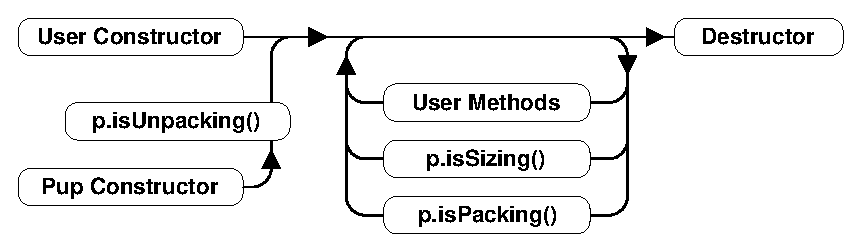
\includegraphics[width=6.0in]{fig/pup}
\end{center}
\caption{Method sequence of an object with a pup method.}
\label{fig:pup}
\end{figure}

Typical method invocation sequence of an object with a pup method is shown in 
Figure~\ref{fig:pup}.  As usual in \CC{}, objects are 
constructed, do some processing, and are then destroyed.

Objects can be created in one of two ways: they can
be created using a normal constructor as usual; or they
can be created using their pup constructor.  The pup constructor
for \charmpp{} array elements and \kw{PUP::able} objects
is a ``migration constructor'' that takes a single ``CkMigrateMessage *";
for other objects, such as parameter marshalled objects,
the pup constructor has no parameters.  The pup constructor
is always followed by a call to the object's pup method in
\verb.isUnpacking. mode.

Once objects are created, they respond to regular user methods
and remote entry methods as usual.  At any time, the object 
pup method can be called in \verb.isSizing. or \verb.isPacking.
mode.  User methods and sizing or packing pup methods can be called
repeatedly over the object lifetime.

Finally, objects are destroyed by calling their destructor
as usual.


\section{Migratable Array Elements using PUP}

\label{arraymigratable}
Array objects can \index{migrate}migrate from one PE to another.  For
example, the load balancer (see section~\ref{lbFramework}) might
migrate array elements to better balance the load between processors.
For an array element to be migratable, it must implement a \uw{pup}
method.  The standard PUP contract (see section \ref{sec:pupcontract})
and constraints wrt to serializing data, and use of Structured Dagger apply.  A simple example for an array follows:

\begin{alltt}
//In the .h file:
class A2 : public CBase\_A2 \{
private: //My data members:
    int nt;
    unsigned char chr;
    float flt[7];
    int numDbl;
    double *dbl;
public:	
    //...other declarations

    virtual void pup(PUP::er \&p);
\};

//In the .C file:
void A2::pup(PUP::er \&p)
\{
    CBase\_A2::pup(p); //<- MUST call superclass's pup method
    p|nt;
    p|chr;
    p(flt,7);
    p|numDbl;
    if (p.isUnpacking()) dbl=new double[numDbl];
    p(dbl,numDbl);
\}
\end{alltt}

\section{Marshalling User Defined Data Types via PUP}

Parameter marshalling requires serialization and is therefore
implemented using the PUP framework.  User defined data types passed
as parameters must abide by the standard PUP contract (see section
\ref{sec:pupcontract}).

For efficiency, arrays are always copied as blocks of bytes and passed
via pointers.  This means classes that need their pup routines to be
called, such as those with dynamically allocated data or virtual
methods cannot be passed as arrays--use CkVec or STL vectors to pass
lists of complicated user-defined classes.  For historical reasons,
pointer-accessible structures cannot appear alone in the parameter
list (because they are confused with messages).

The order of marshalling operations on the send side is:
\begin{itemize}
\item Call ``p\verb.|.a'' on each marshalled parameter with a sizing PUP::er.
\item Compute the lengths of each array.
\item Call ``p\verb.|.a'' on each marshalled parameter with a packing PUP::er.
\item \kw{memcpy} each arrays' data.
\end{itemize}

The order of marshalling operations on the receive side is:
\begin{itemize}
\item Create an instance of each marshalled parameter using its default constructor.
\item Call ``p\verb.|.a'' on each marshalled parameter using an unpacking PUP::er.
\item Compute pointers into the message for each array.
\end{itemize}

Finally, very large structures are most efficiently passed via messages,
because messages are an efficient, low-level construct that minimizes copying
and overhead; but very complicated structures are often most easily passed via 
marshalling, because marshalling uses the high-level pup framework.

See \examplerefdir{PUP/HeapPUP}


  \subsection{Terminal I/O}

\index{input/output}
\charmpp\ provides both C and \CC\ style methods of doing terminal I/O.  

In place of C-style printf and scanf, \charmpp\ provides
\kw{CkPrintf} and \kw{CkScanf}.  These functions have
interfaces that are identical to their C counterparts, but there are some
differences in their behavior that should be mentioned.

A recent change to \charmpp\ is to also support all forms of printf,
cout, etc. in addition to the special forms shown below.  The special
forms below are still useful, however, since they obey well-defined
(but still lax) ordering requirements.

\function{int CkPrintf(format [, arg]*)} \index{CkPrintf} \index{input/output}
\desc{This call is used for atomic terminal output. Its usage is similar to
\texttt{printf} in C.  However, \kw{CkPrintf} has some special properties
that make it more suited for parallel programming on networks of
workstations.  \kw{CkPrintf} routes all terminal output to the \kw{charmrun},
which is running on the host computer.  So, if a
\index{chare}chare on processor 3 makes a call to \kw{CkPrintf}, that call
puts the output in a TCP message and sends it to host
computer where it will be displayed.  This message passing is an asynchronous
send, meaning that the call to \kw{CkPrintf} returns immediately after the
message has been sent, and most likely before the message has actually
been received, processed, and displayed. \footnote{Because of
communication latencies, the following scenario is actually possible:
Chare 1 does a \kw{Ckprintf} from processor 1, then creates chare 2 on
processor 2.  After chare 2's creation, it calls \kw{CkPrintf}, and the
message from chare 2 is displayed before the one from chare 1.}
}

\function{void CkError(format [, arg]*))} \index{CkError} \index{input/output} 
\desc{Like \kw{CkPrintf}, but used to print error messages on \texttt{stderr}.}

\function{int CkScanf(format [, arg]*)} \index{CkScanf} \index{input/output}
\desc{This call is used for atomic terminal input. Its usage is similar to
{\tt scanf} in C.  A call to \kw{CkScanf}, unlike \kw{CkPrintf},
blocks all execution on the processor it is called from, and returns
only after all input has been retrieved.
}

For \CC\ style stream-based I/O, \charmpp\ offers 
\kw{ckout} and \kw{ckerr} in the place of cout, and cerr.  The
\CC\ streams and their \charmpp\ equivalents are related in the same
manner as printf and scanf are to \kw{CkPrintf} and \kw{CkScanf}.  The
\charmpp\ streams are all used through the same interface as the \CC\ 
streams, and all behave in a slightly different way, just like C-style
I/O.

  \section{Other Calls}

\label{other Charm++ calls}

The following calls provide information about the machines upon which the
parallel program is executing.  Processing Element refers to a single CPU.
Node refers to a single machine-- a set of processing elements which share
memory (i.e. an address space).  Processing Elements and Nodes are numbered,
starting from zero.

Thus if a parallel program is executing on one 4-processor workstation and one
2-processor workstation, there would be 6 processing elements (0, 1 ,2, 3, 4,
and 5) but only 2 nodes (0 and 1).  A given node's processing elements are
numbered sequentially.

\function{int CkNumPes()} \index{CkNumPes}
\desc{returns the total number of processors, across all nodes.}

\function{int CkMyPe()} \index{CkMyPe}
\desc{returns the processor number on which the call was made.}

\function{int CkMyRank()} \index{CkMyRank}
\desc{returns the rank number of the processor on which the call was made.
Processing elements within a node are ranked starting from zero.}

\function{int CkMyNode()} \index{CkMyNode}
\desc{returns the address space number (node number) on which the call was made.}

\function{int CkNumNodes()} \index{CkMyNodes}
\desc{returns the total number of address spaces.}

\function{int CkNodeFirst(int node)} \index{CkNodeFirst}
\desc{returns the processor number of the first processor in this address space.}

\function{int CkNodeSize(int node)} \index{CkNodeSize}
\desc{returns the number of processors in the address space on which the call was made.}

\function{int CkNodeOf(int pe)} \index{CkNodeOf}
\desc{returns the node number on which the call was made.}

\function{int CkRankOf(int pe)} \index{CkRankOf}
\desc{returns the rank of the given processor within its node.}

The following calls provide commonly needed functions.

\function{void CkAbort(const char *message)} \index{CkAbort}
\desc{Cause the program to abort, printing the given error message.}

\function{void CkExit()} \index{CkExit}
\desc{This call informs the Charm kernel that computation on all processors
should terminate.  After the currently executing entry method completes, no
more messages or entry methods will be called.  \kw{CkExit} should be the last
call of the entry method from which it was called.}

\function{double CkTimer()} \index{CkTimer} \index{timers}
\desc{returns the current value of the system timer in milliseconds. The system
timer is started when the program begins execution. This timer measures process
time (user and system).}

\function{double CkWallTimer()} \index{CkWallTimer} \index{timers}
\desc{returns the elapsed time since the program has started from the wall
clock timer.}

    
  \subsection{Delegation}

\index{Delegation}
\label{delegation}

{\em Delegation} is a means by which a library writer can 
intercept messages sent via a proxy.  This is typically
used to construct communication libraries.
A library creates a special kind of Group called a 
\kw{DelegationManager}, which receives the messages
sent via a delegated proxy.

There are two parts to the delegation interface-- a
very small client-side interface to enable delegation,
and a more complex manager-side interface to handle
the resulting redirected messages.

\subsubsection{Client Interface}

All proxies (Chare, Group, Array, ...) in \charmpp\ 
support the following delegation routines.

\function{void CProxy::ckDelegate(CkGroupID delMgr);}
Begin delegating messages sent via this proxy to the
given delegation manager. This only affects
the proxy it is called on-- other proxies for the
same object are {\em not} changed. If the proxy is 
already delegated, this call changes the delegation manager.

\function{CkGroupID CProxy::ckDelegatedIdx(void) const;}
Get this proxy's current delegation manager.

\function{void CProxy::ckUndelegate(void);}
Stop delegating messages sent via this proxy.  
This restores the proxy to normal operation.

One use of these routines might be:

\begin{alltt}
  CkGroupID mgr=somebodyElsesCommLib(...);
  CProxy_foo p=...;
  p.someEntry1(...); //Sent to foo normally
  p.ckDelegate(mgr);
  p.someEntry2(...); //Handled by mgr, not foo!
  p.someEntry3(...); //Handled by mgr again
  p.ckUndelegate();
  p.someEntry4(...); //Back to foo
\end{alltt}

The client interface is very simple; but it is often
not called by users directly.  Often the delegate 
manager library needs some other initialization,
so a more typical use would be:

\begin{alltt}
  CProxy_foo p=...;
  p.someEntry1(...); //Sent to foo normally
  startCommLib(p,...); // Calls ckDelegate on proxy
  p.someEntry2(...); //Handled by library, not foo!
  p.someEntry3(...); //Handled by library again
  finishCommLib(p,...); // Calls ckUndelegate on proxy
  p.someEntry4(...); //Back to foo
\end{alltt}

Sync entry methods, group and nodegroup multicast messages,
and messages for virtual chares that have not yet been created
are never delegated.  Instead, these kinds of entry methods
execute as usual, even if the proxy is delegated.

\subsubsection{Manager Interface}

A delegation manager is a group which inherits from
\kw{CkDelegateMgr} and overrides certain virtual methods. 
Since \kw{CkDelegateMgr} does not do any communication itself, 
it need not be mentioned in the
.ci file; you can simply declare a group as usual and
inherit the C++ implementation from \kw{CkDelegateMgr}.

Your delegation manager will be called by \charmpp{}
any time a proxy delegated to it is used.  Since
any kind of proxy can be delegated, there are separate
virtual methods for delegated Chares, Groups, NodeGroups,
and Arrays.

\begin{alltt}
class CkDelegateMgr : public Group {
public:
  virtual void ChareSend(int ep,void *m,const CkChareID *c,int onPE);

  virtual void GroupSend(int ep,void *m,int onPE,CkGroupID g);
  virtual void GroupBroadcast(int ep,void *m,CkGroupID g);

  virtual void NodeGroupSend(int ep,void *m,int onNode,CkNodeGroupID g);
  virtual void NodeGroupBroadcast(int ep,void *m,CkNodeGroupID g);

  virtual void ArrayCreate(int ep,void *m,const CkArrayIndex &idx,int onPE,CkArrayID a);
  virtual void ArraySend(int ep,void *m,const CkArrayIndex &idx,CkArrayID a);
  virtual void ArrayBroadcast(int ep,void *m,CkArrayID a);
  virtual void ArraySectionSend(int ep,void *m,CkArrayID a,CkSectionID &s);
};
\end{alltt}

These routines are called on the send side only.  They are called after 
parameter marshalling; but before the messages are packed.
The parameters passed in have the following descriptions.

\begin{enumerate}
\item{{\bf ep} The entry point begin called, passed as an index into the
\charmpp{} entry table.  This information is also stored in the message's
header; it is duplicated here for convenience.}
\item{{\bf m} The \charmpp{} message.  This is a pointer to the start of the
user data; use the system routine \kw{UsrToEnv} to get the corresponding envelope.
The messages are not necessarily packed; be sure to use \kw{CkPackMessage}.}
\item{{\bf c} The destination \kw{CkChareID}.  This information is already
stored in the message header.}
\item{{\bf onPE} The destination processor number. For chare messages, this
indicates the processor the chare lives on.  For group messages, this indicates
the destination processor.  For array create messages, this indicates the 
desired processor.}
\item{{\bf g} The destination \kw{CkGroupID}.  This is also stored in the 
message header.}
\item{{\bf onNode} The destination node.}
\item{{\bf idx} The destination array index.  This may be looked up using
the lastKnown method of the array manager, e.g., using:
  \begin{alltt}
  int lastPE=CProxy_CkArray(a).ckLocalBranch()->lastKnown(idx);
  \end{alltt} }
\item{{\bf s} The destination array section.}
\end{enumerate}


The \kw{CkDelegateMgr} superclass implements all these methods; so
you only need to implement those you wish to optimize.  You can
also call the superclass to do the final delivery after you've
sent your messages.



    
  \subsection{Communication Optimizations Framework}

The communication framework in Charm++/Converse is aimed at optimizing certain
communication patterns. Currently the programmer has to specify the
communication pattern it intends to optimize, together with the strategy to be
used. The communications library uses the delegation framework
(\ref{delegation}) in order to enable easy and transparent access to the
framework by the programmer.

For \ampi{} programs, the communication optimization is done by the \ampi{}
layer, so that the user does not need to worry about that. In Charm++, however,
the user must create the strategies in the program explicitly. Charm++ programs
are normally based on communicating arrays of chares, that compute and then
invoke entry methods on local or remote chares by sending them messages. These
array elements send messages to each other through proxies. The messages are
passed to the Charm++ runtime which calls lower level network APIs to
communicate. To optimize communication in Charm++, the user can redirect a
communication {\em call} to go through an instance of a strategy.

To access the communication framework, the user first creates and initializes a
communication library strategy. He then needs to make a copy of the array proxy
and associate it with that strategy. In order to use the framework, the
receiving entry methods need to receive messages (see \ref{messages}), and not
marshalled parameters. The user can create several instances of the same or
different strategies, to optimize different communication calls in the
application. In order to access the class signatures, the file ``comlib.h''
should be included.

Each communication operation is associated with a proxy, through which the
message is sent. These proxies can be associated in the mainchare constructor
(useful for all-to-all strategies), or later in the single chare
array elements (useful for section multicasts). In both cases, some
information has to be kept, either the CProxy or the ComlibInstanceHandle, and
this can be done in readonly variables, or as internal variables of the objects.

An example on how to use commlib can be found in the charm distribution, under
``examples/charm++/commlib/multicast/ '', where the proxies are associated in the
chare arrays.


\subsubsection{Using commlib}

One thing typically useful is having the the proxy associated with the strategy,
or an instance of the strategy (to be used for future associations) to be
declared as readonly variable, although this in not necessary. This is done by
declaring them readonly (see \ref{readonly} for more information).

\begin{alltt}
  readonly CProxy\_MyArray aproxy;
  readonly CProxy\_MyArray comlibproxy;
  readonly ComlibInstanceHandle cinst;
\end{alltt}

The creation of all the strategies needed, and their registration must be done
in the constructor of the mainchare (for more on array creation see
\ref{advanced array create}):

\begin{alltt}
  // Create the array
  aproxy = CProxy\_MyArray::ckNew();

  // Create the strategy (description of constructors later)
  CharmStrategy *strategy = new EachToManyMulticastStrategy(USE_MESH, srcarray, destarray);
  //or
  CharmStrategy *strategy = new StreamingStrategy(10,10);

  // Either associate the strategy with the proxy we declared, or register the
  // strategy to commlib for future association, or both.
  comlibproxy = aproxy;
  ComlibAssociateProxy(strategy, comlibproxy);

  cinst = ComlibRegister(strategy);
\end{alltt}

In this example, after aproxy has been associated with comlibproxy it can only be
used with commlib, and cannot send anymore regular messages. For this, if
regular messages without commlib are desired, a copy of the original proxy
should be made (like here).

In the chare array element, if {\texttt{cinst}} has been defined, other proxies
can be created and associated, like here a CProxySection\_MyArray, which allows
to send multicasts (see \ref{array section} for more on section proxies).

\begin{alltt}
  CProxySection\_MyArray mysection = .....
  ComlibAssociateProxy(cinst, mysection);  // mysection will always use commlib
\end{alltt}

After a proxy has been associated in some way to commlib, it can be used to send
messages with commlib:

\begin{alltt}
  comlibproxy.receive(msg); // send with commlib
  mysection.compute(msg);   // send to a section with commlib

  aproxy[0].single(msg);    // send to a single element {\textbf{without}} commlib
\end{alltt}

In case a bracketed strategy is used, two additional function calls have to
be added before starting to send the messages and after finishing. These are
discussed later in \ref{bracketed strategies}.

The signatures of the functions used here are the following:

\begin{alltt}
ComlibRegister (CharmStrategy *strat);
ComlibAssociateProxy (CharmStrategy *strat, CProxy &proxy);
ComlibAssociateProxy (ComlibInstanceHandle *cinst, CProxy &proxy);
\end{alltt}

%% \subsubsection{Proxy interface}

%% A proxy containing the delegation should be kept, and reused every time the
%% associated stragety wants to be used.

%% \begin{enumerate}
%% \item main.C global
%% \begin{alltt}
%% // Include the appropriate header file
%% #include <EachToManyMulticastStrategy.h>
%% #include <StreamingStrategy.h>

%% // Declare the global variable
%% CProxy_MyArray aproxy;
%% CProxy_MyArray dproxy;
%% \end{alltt}

%% \item main.C:main()
%% \begin{alltt}
%% // Create the array
%% aproxy = CProxy_Hello::ckNew();

%% // Create the strategy (description of constructors later)
%% CharmStrategy *strategy = new EachToManyMulticastStrategy(USE_MESH, srcarray, destarray);
%% //or
%% CharmStrategy *strategy = new StreamingStrategy(10,10);

%% // Register the strategy to a new proxy, so that aproxy is without commlib,
%% // while dproxy uses it
%% dproxy = aproxy;
%% ComlibAssociateProxy(strategy, dproxy);
%% \end{alltt}

%% \item In the array element
%% \begin{alltt}
%% // First proxy should be delegated
%% ComlibBeginIteration(dproxy);   // Only for bracketed strategies
%% dproxy[index].entry(message);   // Sending a message
%% .....     //sending more messages
%% .....
%% aproxy[index].entry2{message2); // Send a message without commlib
%% ComlibEndIteration(dproxy);     // Only for bracketed strategies
%% \end{alltt}
%% \end{enumerate}

%% The above example shows the usage of EachToManyStrategy. Notice the
%% ComlibBeginIteration and ComlibEndIteration calls, needed for bracketed
%% strategies. The construction of the strategies has been done in tha main::main,
%% from where they are broadcasted and initialized in every processor before being
%% used.

%% \subsubsection{Instance interface}

%% In this interface, the chares need to keep information about the commlib instance.

%% \begin{enumerate}
%% \item main.C global
%% \begin{alltt}
%% // Include the appropriate header file
%% #include <EachToManyMulticastStrategy.h>
%% #include <StreamingStrategy.h>

%% // Declare the global variable
%% CProxy_MyArray aproxy;
%% ComlibInstanceHandle cinst;
%% \end{alltt}

%% \item main.C:main()
%% \begin{alltt}
%% // Create the array
%% aproxy = CProxy_Hello::ckNew();

%% // Create your strategy
%% Strategy *strategy = new EachToManyStrategy(USE_MESH, srcarray, destarray);
%% //or
%% Strategy *strategy = new StreamingStrategy(10,10);

%% // Create a Communication Library Instance
%% cinst = CkGetComlibInstance();

%% // Register the strategy
%% cinst.setStrategy(strategy);
%% \end{alltt}

%% \item In the array element 
%% \begin{alltt}
%% // Before calling an entry method whose message should go thorough the
%% // library the proxy has to be delegated. Create a new copy of the
%% // proxy and delegate it before using it.
%% CProxy_Hello dproxy = aproxy;
%% ComlibDelegateProxy(&dproxy); //Now all calls to dproxy will go through the library.

%% cinst.beginIteration();       // Only for bracketed strategies
%% dproxy[index].entry();        // Send a message
%% .....
%% .....
%% aproxy[index].entry2();       // Send a message without commlib
%% cinst.endIteration();         // Only for bracketed strategies
%% \end{alltt}
%% \end{enumerate}

%% \subsubsection{Sections}

%% In order to multicast only to a part of the array instead of the entire array,
%% it is necessary to create a {\textrm{CProxySection\_class}}
%% (\ref{array_section_multicast}) of the desired portion of the destination array,
%% delegate it with {\textrm{ComlibAssociateProxy()}}, and send a broadcast to it.
%% This broadcast on the section will result in the desired multicast on the global
%% array. Only multicast strategies can be used for this.


\subsubsection{Loadbalancing and Migration support}

The Communication optimization framework supports both loadbalancing and array
migration. It enables migration through message forwarding. Messages sent by a
migrated array are forwarded to the processor where it is mapped to, and from
here they get accounted. Messages sent to migrated arrays are forwarded from the
processor where they are mapped to their current destination.

This mapping of array elements to processors can be updated by the user by
calling {\textrm{ComlibResetProxy}} for array proxies, and
{\textrm{ComlibResetSectionProxy}} for section proxies. This should be done
especially during load-balancing, where most of the migrations happen. As shown
in the following example, these calls should be made inside the
{\textrm{resumeFromSync}} method.

\begin{alltt}
  void arrayelement::resumeFromSync() {
      .......
      .......
      ComlibResetProxy(comlibproxy);
      ComlibResetSectionProxy(mysection);
  }
\end{alltt}

A migrating array element containing {\em associated proxies} or {\em
instances} should pup them all at the source and destination.

\begin{alltt}
  void arrayelement::pup(PUP::er &p){
      ..........
      ..........
      p | mysection;
      p | cinst;
  }
\end{alltt}

\subsubsection{Compiling User Code}

All user programs that use the communication library should use the
linker option {\textrm{-module comlib}. For example,
\begin{alltt}
charmc -o pgm pgm.o -module comlib
\end{alltt}


\subsubsection{Supported Operations and Strategies}

The communication framework now supports four different communication
operations:
\begin{enumerate}
\item all-to-all/many-to-many communication,
\item array and group broadcast,
\item section multicast,
\item streaming.
\end{enumerate}
Table~\ref{tbl:com_operation} shows the different strategies that optimize these
communication operations. Some of these are converse strategies while others are
charm strategies. In the following paragraphs, we present in detail the
strategies optimizing the above mentioned operations.

\begin{table}[h]
\begin{center}
\begin{small}
\begin{tabular}{|c|c|c|}
\hline
{\bf Operation} & {\bf Object Strategy} & {\bf Processor Strategy} \\
\hline
\begin{tabular}{c}
All-to-All/Many-to-many \\
personalized and multicast
\end{tabular}
 & EachToManyMulticastStrategy & Mesh, Grid, Hypercube, Direct \\
%Many-to-many  multicast    & EachToManyMulticastStrategy & Mesh, Grid, Hypercube, Direct \\
Broadcast  & BroadcastStrategy, PipeBroadcastStrategy & Binomial tree, Binary tree\\
Section Multicast &
\begin{tabular}{c}
DirectMulticastStrategy, RingMulticastStrategy,\\
MultiRingMulticast
\end{tabular} & \\
Streaming  & Streaming, MeshStreaming, PrioStreaming & \\
\hline
\end{tabular}
\end{small}
\end{center}
\caption{Communication Operations supported in the Framework}
\label{tbl:com_operation}
\end{table}

There are two types of strategies in the communication framework:

\begin{itemize}

\item \label{bracketed strategies}
Bracketed Strategies: In bracketed strategies each source chare (which could be
an array element or a group) deposits its entries and then the strategy performs
the communication optimization. For example the EachToManyMulticastStrategy is a
bracketed strategy. For bracketed strategies a beginIteration and an
endIteration must be called before and after making the deposits respectively.

The usage of the strategy becomes:

\begin{alltt}
ComlibBegin(dproxy);

dproxy[index].entry(message);   // Sending a message
.....     //sending more messages
.....

ComlibEnd(dproxy);
\end{alltt}

\item Non-Bracketed Strategies: Non-bracketed strategies perform communication
optimizations without needing calls to beginIteration and endIteration to start
processing. Non-bracketed strategies either immediately process messages or
after a timeout, and, in both cases, it's not triggered from the application.

\end{itemize}


\subsubsection{Many-to-many Strategies}

The class {\em EachToManyMulticastStrategy} optimizes both all-to-all
personalized and all-to-all multicast communication using several virtual
topologies like 2-D Mesh, 3-D Mesh and Hypercube. Personalized communication
happens when a chare sends different messages to the other chares, multicast
communication happens when a chare sends the same message to all other chares.
EachToManyMulticastStrategy also optimizes the special cases of many-to-many multicast where
not all the chares in an array are involved in the collective operation.

The charm level strategy collects all the messages from the chares and delivers
them to the destination, while the low level (processor-to-processor)
communication is performed through converse level {\em routers} and
implements the various virtual topologies.

%For example, with the mesh router, the strategy on each processor
%first sends messages to its row neighbors. After having received its row
%messages each processor sends the column messages. After having received the
%column messages an iteration of the strategy finishes. All local messages are
%delivered as soon they are received.

%{\em EachToManyMulticastStrategy} is also used to optimize all-to-all multicast
%communication, where a processor sends the same message to all others, using the
%same virtual topologies at the lower level.

EachToManyMulticastStrategy requires that all local messages be deposited
before they can be packed into single messages. Hence, it needs to be a {\em
bracketed} strategy. This strategy can also be used to optimize all-to-all collectives between charm
groups.

%Bracketed strategies require each of the participating objects to deposit their
%intended messages within brackets. Calls to {\em ComlibBeginIteration} and {\em
%ComlibEndIteration} create a bracket. The call ComlibBeginIteration sets up the
%delegation framework to forward user messages to the correct strategy instance.
%User messages then get passed to the insertMessage entry function of the
%strategy. When all local objects have called ComlibEndIteration, doneInserting
%is invoked on the strategy.

%Bracketed strategies are typically needed when the communication
%optimization requires local source objects to reach a barrier. At this
%local barrier the communication framework invokes doneInserting on
%that strategy, which the calls the converse level strategy.

%Non-bracketed strategies have no such restriction. They process
%messages as soon as they arrive. so, non-bracketed strategies should
%not expect a doneInserting to be invoked on them. They must all
%process messages in the insertMessage call itself.

As for the constructors to be used in the main chare, the two prototypes follow.
The first one is for groups, the second for arrays. The optional parameters
allow to specify the many-to-many behaviour, passing the lists of source and
destination elements participating in the operation. If they are left to the
default value, the collective is an all-to-all.

\begin{alltt}
EachToManyMulticastStrategy(int substrategy, int nsrcpes=0, int *srcpelist=0,
                            int ndestpes=0, int *destpelist=0);

EachToManyMulticastStrategy(int substrategy, CkArrayID src, CkArrayID dest,
                            int nsrc=0, CkArrayIndexMax *srcelements=0,
                            int ndest=0, CkArrayIndexMax *destelements=0);
\end{alltt}

Both have as first parameter the virtual topology that the strategy will use for
the low level optimization. The possible values are:

\begin{description}
\item[USE\_DIRECT] to send messages directly;
\item[USE\_MESH] to send messages across a 2D Mesh;
\item[USE\_GRID] to send messages across a 3D Grid;
\item[USE\_HYPERCUBE] to send messages across a Hypercube.
\end{description}

USE\_HYPERCUBE will do best for very small messages and small number of
processors, 3d has better performance for slightly higher message sizes and then
Mesh starts performing best. The programmer is encouraged to try out all the
topologies.


\subsubsection{Broadcast Strategies}

There are two strategies of this type: {\em BroadcastStrategy} and {\em
PipeBroadcastStrategy}. The first works only for group broadcast, while the
second works for both groups and arrays.

BroadcastStrategy performs a broadcast through a hypercube (default) or a tree,
and the constructor is:

\begin{alltt}
BroadcastStrategy(int topology=USE_HYPERCUBE);
\end{alltt}

PipeBroadcastStrategy performs a broadcast through a ring or a hypercube
(default). The characteristic of this strategy is that it fragments the message
into small chunks that fit a predetermined size (passed as argument to the
constructor), and it reassembles them before delivery. The constructor
prototypes for groups and arrays respectively are:

\begin{alltt}
PipeBroadcastStrategy(int topology, CkArrayID aid, int pipeSize=DEFAULT_PIPE);
PipeBroadcastStrategy(CkGroupID gid, int topology=USE_HYPERCUBE, int pipeSize=DEFAULT_PIPE);
\end{alltt}


\subsubsection{Section Multicast Strategies}

The subclasses of MulticastStrategy can multicast a message to the entire array
or a section of array elements (MulticastStrategy itself is abstract). The
multicast strategies are non-bracketed, and the message is processed when the
application deposits it. These strategies do not combine messages, but they may
sequence the destinations of the multicast to minimize contention on a network.

In order to use these strategies, the message sent must inherit from class
{\textrm{CkMcastBaseMsg}}. (For an example see
``examples/charm++/commlib/multicast/'').

These are the subclass strategies that are available:

\begin{description}
\item[DirectMulticastStrategy] sends the messages directly to all recipients;
\item[RingMulticastStrategy] sends the messages along ring resulting in good throughput as the ring permutation is contention free on many communication topologies;
\item[MultiRingMulticast] sends the message along two rings (the ordered list of recipients is split in half).
\end{description}

For these, the constructors are of the form:

\begin{alltt}
DirectMulticastStrategy(CkArrayID aid, int flag=0);
RingMulticastStrategy(CkArrayID dest_id, int flag=0);
MultiRingMulticast(CkArrayID dest_id, int flag=0);
\end{alltt}

For section multicast, the user must create a section proxy and delegate it to
the communication library. Invocations on section proxies are passed on to the
section multicast strategy.


\subsubsection{Streaming Strategies}

This strategy optimizes the scenario where chares send several small messages to
other chares. The StreamingStrategy collects messages destined to the same
physical processor and, after a timeout or when a certain number of messages
have been collected, it sends them as a single message. This results in sending
fewer messages of larger size. The timeout is a floating-point parameter to the
StreamingStrategy. It needs to be specified in milliseconds, with a default
value of 1ms. Micro-second timeouts can also be specified by passing values less
than 1. For example, $0.1$ represents $100\mu s$.

The Streaming Strategy is a non-bracketed strategy. Since messages can be
delayed due to the timeout present, it is possible to call
{\textrm{ComlibEnd()}} to flush all the messages to be sent immediately.

The prototype of the constructor is:

\begin{alltt}
StreamingStrategy(float period\_in\_ms, int nmsgs);
\end{alltt}

There are two variants of this strategy:

\begin{description}
\item[MeshStreamingStrategy] which sends the messages along a mesh instead of a linear array as the basic one;
\item[PrioStreaming] which looks at the priority of the messages, and sends those with a priority above a certain threshold directly, without delay. This strategy accepts a third parameter in the constructor for the threshold priority.
\end{description}


\subsubsection{Communication Optimization Development}

Optimization algorithms are implemented as Strategies in the communication
library. Strategies can be implemented at the Object (\charmpp) level or the
processor (\converse) level. Code reuse is possible by having a few object
managers perform object level optimizations and then call several other
processor level optimization schemes. For example, to optimize all-to-all
communication the processor level strategies could use the different virtual
topologies.

All processor (\converse) level strategies inherit from the {\em class~Strategy}
defined below and override its virtual methods.

\begin{alltt}
// Converse or Processor level strategy
class Strategy : public PUP::able{
public:
    // Called for each message
    virtual void insertMessage(MessageHolder *msg);
    // Called after all chares and groups have finished depositing their
    // messages on that processor.

    virtual void doneInserting();
    virtual void beginProcessing(int nelements);
};
\end{alltt}

The class method {\em insertMessage} is called to deposit messages with the
strategy. MessageHolder is a wrapper for converse messages. When a processor has
sent all its messages {\em doneInserting} is invoked on the strategy.

At the \charmpp{} level, all strategies inherit from the {\em
class~CharmStrategy} reported here.

\begin{alltt}
// Charm++ or Object level strategy
class CharmStrategy : public Strategy{
 protected:
    int isArray;
    int isGroup;
    int isStrategyBracketed;
    ............   
    ............   
public:
    // Called for each message
    virtual void insertMessage(CharmMessageHolder *msg);
    // Called after all chares and groups have finished depositing their
    // messages on that processor.
    virtual void doneInserting();
    virtual void beginProcessing(int nelements);
};
\end{alltt}

\charmpp{} level strategies also have to implement the insertMessage and
doneInserting methods. Here insertMessage takes a CharmMessageHolder which is a
\charmpp{} message wrapper. The call to beginProcessing initializes the strategies
on each processor. This additional call is needed because the constructor of the
strategy is called by user code in main::main on processor 0, while the strategy
needs to be constructed everywhere. Along with initializing its data,
beginProcessing can also register message handlers, as the communication library
strategies use Converse handlers to communicate between processors. The flags
{\em isArray} and {\em isGroup} store the type of objects that call the strategy
and the flag {\em isStrategyBracketed} specifies if the CharmStrategy is
bracketed or not. Bracketed strategies require that the application deposits
messages in brackets demarcated by the calls ComlibBegin and
ComlibEnd.

  \subsection{All-to-All}

All-to-All is a frequently encountered pattern of communication in
parallel programs where each processing element sends a message to
every other processing element. Variations on this pattern are also
common. A processing element may want to send multiple messages to the
same destination over time, for example, and not every pair of
processors may need to communicate. In Charm++ we classify these
scenarios under a single API with the aim of improving any type of
Many-to-Many communication pattern.

Note that we are currently extending support for All-to-All
communication in Charm++ and so the API may change in the
future. 

\subsubsection{MeshStreamer}

MeshStreamer optimizes the case of All-to-All and Many-to-Many
communication on regular 2D and 3D machine topologies. Messages sent
using MeshStreamer are routed along the dimensions of the specified
topology and aggregated at intermediate destinations. When using it,
the first step is to create a MeshStreamer group. 

\begin{alltt}
MeshStreamer(int totalBufferCapacity, int numRows, 
             int numColumns, int numPlanes, 
             const CProxy_MeshStreamerClient<dtype> &clientProxy,
             int yieldFlag = 0, int progressPeriodInMs = -1);
\end{alltt}

The constructor takes as input a reference to a MeshStreamerClient
proxy. The user should pass in the proxy for the group which will
receive the data sent using MeshStreamer. To do so, this group should
inherit from the MeshStreamerClient group. Note that MeshStreamer and
MeshStreamerClient are templated. The templated parameter specifies
the type of data units which will be communicated. 

The totalBufferCapacity parameter for the MeshStreamer constructor
specifies the buffering limit of the library. When the collective
number of items buffered by the local instance of the group reaches
the specified limit, the library sends a message along each dimension
to the destination for which it has buffered the most messages.

MeshStreamer employs a virtual topology to route messages. The
topology is specified by the user. When a regular mesh partition is
avilable for execution, performance will be much better if the
dimensions of the virtual topology submitted by the user correspond to
the physical dimensions of the machine topology. The Charm++ Topology
Manager can be used to produce this information for the user at run
time. 

The insertData function, best used when called on the local instance
of the MeshStreamer group, hands over individual units of data for
transmission by the library. 

\begin{alltt}
void insertData(dtype &dataItem, const int destinationPe); 
\end{alltt}

To receive items, the user needs to define a process function, which
is a pure virtual function of MeshStreamerClient.

\begin{alltt}
virtual void process(dtype &data)=0; 
\end{alltt}

MeshStreamer aggregates items into messages which are sent out when
internal buffers fill up or periodic time limits are reached. The
message arriving at the destination index of the MeshStreamer group
may contain items from various group indices. The receiveCombinedData
function loops over the received items and calls the process function
for each item. The user may choose to redefine this function to
specify an alternate message processing behavior. 

\begin{alltt}
virtual void receiveCombinedData(MeshStreamerMessage<dtype> *msg);
\end{alltt}


  \subsection{Python scripting language}

\label{python}

The Python scripting language in \charmpp{} allows the user to dynamically
execute pieces of code inside a running application, without the need to
recompile. This is performed through the CCS (Converse Client Server) framework
(see ``Converse Manual'' for more information about this). The user specifies
which elements of the system will be accessible through the interface, as we
will see later, and then run a client which connects to the server.

In order to exploit this functionality, Python interpreter needs to be installed
into the system, and \charmpp{} LIBS need to be built with:\\
\texttt{./build LIBS $<$arch$>$ $<$options$>$}

The interface provides three different types of requests:

\begin{description}
\item[Execute] requests to execute a code, it will contain the code to be executed on the server, together with the instructions on how to handle the environment;
\item[Print] asks the server to send back all the strings which has been printed by the script until now;
\item[Finished] asks the server if the current script has finished or it is still running.
\end{description}

There are three modes to run code on the server, ordered here by increase of
functionality, and decrease of dynamic flexibility:
\begin{itemize}
\item \textbf{simple read/write} By implementing the \kw{read} and \kw{write} methods
of the object exposed to python, in this way single variables may be exposed,
and the code will have the possibility to modify them individually as desired.
(see section~\ref{pythonServerRW})
\item \textbf{iteration} By implementing the iterator functions in the server (see
\ref{pythonServerIterator}), the user can upload the code of a Python function
and a user-defined iterator structure, and the system will apply the specified
function to all the objects reflected by the iterator structure.
\item \textbf{high level} By implementing \kw{python} entry methods, the Python code uploaded can access them and activate complex, parallel operations that will be performed by the \charmpp{} application. (see section~\ref{pythonHighLevel})
\end{itemize}

The description will follow the client implementation first, and continuing then
on the server implementation.


\subsubsection{The client side}

\label{pythonClient}

In order to facilitate the interface between the client and the server, some
classes are available to the user to include into the client. Currently \CC{} and
java interfaces are provided.

\CC{} programs need to include \texttt{PythonCCS-client.h} into their
code. This file is among the \charmpp{} include files. For java, the package
\texttt{charm.ccs} needs to be imported. This is located under the java
directory on the \charmpp{} distribution, and it provides both the Python and
CCS interface classes.

There are three main classes provided: \texttt{PythonExecute},
\texttt{PythonPrint}, and \texttt{PythonFinished} which are used for the three
different types of request.

All of them have two common methods to enable communication across different platforms:

\begin{description}

\item[int size();]
Returns the size of the class, as number of bytes that will be
transmitted through the network (this includes the code and other dynamic
variables in the case of \texttt{PythonExecute}).

\item[char *pack();]
Returns a new memory location containing the data to be sent to the server, this
is the data which has to be passed to the \texttt{CcsSendRequest} function. The
original class will be unmodified and can be reused in subsequent calls.

\end{description}

A tipical invocation to send a request from the client to the server has the
following format:

\begin{alltt}
CcsSendRequest (&server, "pyCode", 0, request.size(), request.pack());
\end{alltt}

\subsubsection{PythonExecute}

\label{pythonExecute}

To execute a Python script on a running server, the client has to create an
instance of \texttt{PythonExecute}, the two constructors have the following
signature (java has a correspondent functionality):

\begin{alltt}
PythonExecute(char *code, bool persistent=false, bool highlevel=false, CmiUInt4 interpreter=0);
PythonExecute(char *code, char *method, PythonIterator *info, bool persistent=false,
              bool highlevel=false, CmiUInt4 interpreter=0);
\end{alltt}

The second one is used for iterative requests (see~\ref{pythonIterator}). The
only required argument is the code, a null terminated string, which will not be
modified by the system. All the other parameters are optional. They refer to the
possible variants that an execution request can be. In particular, this is a
list of all the options present:

\begin{description}

\item[iterative]
If the request is a single code (false) or if it represents a function over
which to iterate (true) (see~\ref{pythonIterator} for more details).

\item[persistent]
It is possible to store information on the server which will be retained across
different client calls (such as simple data or complete libraries). True means
that the information will be retained on the server, false means that the
information will be deleted when the script terminates to run. In order to
properly dispose the memory, when the last call is made (and the data is not
anymore needed), this flag should be set to false. When information has been
stored on the server, in order to reuse it, the interpreter field of the request
should be set to the correct value (which was returned by the previous call, see
later in this subsection).

\item[high level]
In order to have the ability to call high level \charmpp{} functions (available
through the keywork \kw{python}) this flag must be set to true. If it is false,
the entire module ``charm'' will not be present, but the startup of the script
will be faster.

\item[print retain]
When the client decides to print some output back to the client, this data can be
retrieved with a PythonPrint request. If the output is not desired, this flag
can be set to false, and the output will be discarded. If it is set to true the
output will be saved waiting to be retrieved by the client. The data will
survive also after the termination of the Python script, and if not retrieved
will waste memory on the server.

\item[busy waiting]
Instead of returning immediately to the client a handle that can be used to
retrieve prints and check if the script has finished, the server will answer to
the client only when the script has terminated to run (and it will effectively
work as a PythonFinished request).

\end{description}

These flags can be set and checked with the following routines (CmiUInt4 represent a 4
byte unsigned integer):

\begin{alltt}
void setCode(char *set);
void setPersistent(bool set);
void setIterate(bool set);
void setHighLevel(bool set);
void setKeepPrint(bool set);
void setWait(bool set);
void setInterpreter(CmiUInt4 i);

bool isPersistent();
bool isIterate();
bool isHighLevel();
bool isKeepPrint();
bool isWait();
CmiUInt4 getInterpreter();
\end{alltt}

From a PythonExecute request, the server will answer with a 4 byte integer
value, which is a handle for the interpreter that is running. It can be used to
request for prints, check if the script has finished, and for reusing the same
interpreter (if it was persistent).

A value of 0 means that there was an error and the script didn't run. This is
typically due to a request to reuse of an existing interpreter which is not
available, either because it was not persistent or because another script is
still running on that interpreter.


\subsubsection{Auto-imported modules}

\label{pythonModules}

When a Python script is run inside a \charmpp{} application, two Python modules
are made available by the system. One is \textbf{ck}, the other is
\textbf{charm}. The first one is always present and it represent basic
functions, the second is related to high level scripting and it is present only
when this is enabled (see \ref{pythonExecute} for how to enable it, and
\ref{pythonHighLevel} for a description on how to implement charm functions).

The methods present in the \texttt{ck} module are the following:

\begin{description}

\item[printstr]
It accepts a string as parameter. It will write into the server stdout that string
using the \texttt{CkPrintf} function call.

\item[printclient]
It accepts a string as parameter. It will forward the string back to the client when it
issues a PythonPrint request. It will buffer the strings if the \texttt{KeepPrint}
option is true, otherwise it will discard them.

\item[mype]
It requires no parameters, and it will return an integer representing the
current processor where the code is executing. It is equivalent to the \charmpp{}
function \texttt{CkMyPe()}.

\item[numpes]
It requires no parameters, and it will return an integer representing the
total number of processors that the application is using. It is equivalent to
the \charmpp{} function \texttt{CkNumPes()}.

\item[myindex]
It requires no parameters, and it will return the index of the current element
inside the array, if the object under which Python is running is an array, or
None if it is running under a Chare, a Group or a Nodegroup. The index will be a
tuple containing as many numbers as the dimension of the array.

\item[read]
It accepts one object parameter, and it will perform a read request to the
\charmpp{} object connected to the Python script, and return an object
containing the data read (see \ref{pythonServerRW} for a description of this
functionality). An example of a call can be:
\function{value = ck.read((number, param, var2, var3))}
where the double parenthesis are needed to create a single tuple object
containing four values passed as a single paramter, instead of four different
parameters.

\item[write]
It accepts two object parameters, and it will perform a write request to the
\charmpp{} object connected to the Python script. For a description of this
method, see \ref{pythonServerRW}. Again, only two objects need to be passed, so
extra parenthesis may be needed to create tuples from individual values.

\end{description}

\subsubsection{Iterate mode}

\label{pythonIterator}

Sometimes some operations need to be iterated over all the elements in the
system. This ``iterative'' functionality provides a shortcut for the client user
to do this. As an example, suppose we have a system which contains particles,
with their position, velocity and mass. If we implement \texttt{read} and
\texttt{write} routines which allow us to access single particle attributes, we may
upload a script which doubles the mass of the particles with velocity greater
than 1:

\begin{alltt}
size = ck.read((``numparticles'', 0));
for i in range(0, size):
    vel = ck.read((``velocity'', i));
    mass = ck.read((``mass'', i));
    mass = mass * 2;
    if (vel > 1): ck.write((``mass'', i), mass);
\end{alltt}

Instead of all these read and writes, it will be better to be able to write:

\begin{alltt}
def increase(p):
    if (p.velocity > 1): p.mass = p.mass * 2;
\end{alltt}

This is what the ``iterative'' functionality provides. In order for this to
work, the server has to implement two additional functions
(see~\ref{pythonServerIterator}), and the client has to pass some more
information together with the code. This information is the name of the function
that has to be called (which can be defined in the ``code'' or have already been
uploaded to a persistent interpreter), and a user defined structure which
specifies over what data the function should be invoked. These values can be
specified either while constructing the PythonExecute variable (see the second
constructor in section~\ref{pythonExecute}), or with the following methods:

\begin{alltt}
void setMethodName(char *name);
void setIterator(PythonIterator *iter);
\end{alltt}

As for the PythonIterator object, it has to be a class defined by the user, and
the user has to insure that the same definition is present inside both the
client and the server. The \charmpp{} system will simply pass this structure as
a void pointer. This structure needs to inherit from \texttt{PythonIterator}. It
is recommended that no pointers are used inside this class, and no dynamic
memory allocation. If this is the case, nothing else needs to be done.

If instead pointers and dynamic memory allocation is used, the following methods
have to be reimplemented:

\begin{alltt}
int size();
char * pack();
void unpack();
\end{alltt}

The first returns the size of the class/structure after being packed. The second
returns a pointer to a newly allocated memory containing all the packed data,
the returned memory must be compatible with the class itself, since later on
this same memory a call to unpack will be performed. Finally, the third will do
the work opposite to pack and fix all the pointers. This method will not return
anything and is supposed to fix the pointers ``inline''.

\subsubsection{PythonPrint}

\label{pythonPrint}

In order to receive the output printed by the Python script, the client needs to
send a PythonPrint request to the server. The constructor is:

\function{PythonPrint(CmiUInt4 interpreter, bool Wait=true, bool Kill=false);}

The interpreter for which the request is made is mandatory. The other parameters
are optional. The wait parameter represents whether a reply will be sent back
immediately to the client even if there is no output (false), or if the answer
will be delayed until there is an output (true). The \kw{kill} option set to
true means that this is not a normal request, but a signal to unblock the latest
print request which was blocking.

The returned data will be a non null-terminated string if some data is present
(or if the request is blocking), or a 4 byte zero data if nothing is present.
This zero reply can happen in different situations:

\begin{itemize}
\item If the request is non blocking and no data is available on the server;
\item If a kill request is sent, the previous blocking request is squashed;
\item If the Python code ends without any output and it is not persistent;
\item If another print request arrives, the previous one is squashed and the second one is kept.
\end{itemize}

As for a print kill request, no data is expected to come back, so it is safe to
call \texttt{CcsNoResponse(server)}.

The two options can also be dynamically set with the following methods:

\begin{alltt}
void setWait(bool set);
bool isWait();

void setKill(bool set);
bool isKill();
\end{alltt}

\subsubsection{PythonFinished}

\label{pythonFinished}

In order to know when a Python code has finished executing, especially when
using persistent interpreters, and a serialization of the scripts is needed, a
PythonFinished request is available. The constructor is the following:

\function{PythonFinished(CmiUInt4 interpreter, bool Wait=true);}

The interpreter corresponds to the handle for which the request was sent, while
the wait option refers to a blocking call (true), or immediate return (false).

The wait option can be dynamically modified with the two methods:

\begin{alltt}
void setWait(bool set);
bool isWait();
\end{alltt}

This request will return a 4 byte integer containing the same interpreter value
if the Python script has already finished, or zero if the script is still
running.

\subsubsection{The server side}

\label{pythonServer}

In order for a \charmpp{} object (chare, array, node, or nodegroup) to receive
python requests, it is necessary to define it as python-compliant. This is done
through the keyword \kw{python} placed in square brackets before the object name
in the .ci file. Some examples follow:

\begin{alltt}
mainchare [python] main \{\ldots\}
array [1D] [python] myArray \{\ldots\}
group [python] myGroup \{\ldots\}
\end{alltt}

In order to register a newly created object to receive Python scripts, the
method \texttt{registerPython} of the proxy should be called. As an example,
the following code creates a 10 element array myArray, and then registers it to
receive scripts directed to ``pycode''. The argument of \texttt{registerPython}
is the string that CCS will use to address the Python scripting capability of
the object.

\begin{alltt}
Cproxy_myArray localVar = CProxy_myArray::ckNew(10);
localVar.registerPython(``pycode'');
\end{alltt}


\subsubsection{Server \kw{read} and \kw{write} functions}

\label{pythonServerRW}

As explained previously in subsection~\ref{pythonModules}, some functions are
automatically made available to the scripting code through the {\em ck} module.
Two of these, \textbf{read} and \textbf{write} are only available if redefined
by the object. The signatures of the two methods to redefine are:

\begin{alltt}
PyObject* read(PyObject* where);
void write(PyObject* where, PyObject* what);
\end{alltt}

The read function receives as a parameter an object specifying from where the data
will be read, and returns an object with the information required. The write
function will receive two parameters: where the data will be written and what
data, and will perform the update. All these \texttt{PyObject}s are generic, and
need to be coherent with the protocol specified by the application. In order to
parse the parameters, and create the value of the read, please refer to the
manual \htmladdnormallink{``Extending and Embedding the Python Interpreter''}{http://docs.python.org/}, and in particular to the functions
\texttt{PyArg\_ParseTuple} and \texttt{Py\_BuildValue}.

\subsubsection{Server iterator functions}

\label{pythonServerIterator}

In order to use the iterative mode as explained in
subsection~\ref{pythonIterator}, it is necessary to implement two functions
which will be called by the system. These two functions have the following
signatures:

\begin{alltt}
int buildIterator(PyObject*, void*);
int nextIteratorUpdate(PyObject*, PyObject*, void*);
\end{alltt}

The first one is called once before the first execution of the Python code, and
receives two parameters. The first is a pointer to an empty PyObject to be filled with
the data needed by the Python code. In order to manage this object, some utility
functions are provided. They are explained in subsection~\ref{pythonUtilityFuncs}.

The second is a void pointer containing information of what the iteration should
run over. This parameter may contain any data structure, and an agreement between the
client and the user object is necessary. The system treats it as a void pointer
since it has no information of what user defined data it contains.

The second function (\texttt{nextIteratorUpdate}) has three parameters. The
first contains the object to be filled like in \texttt{buildIterator}, but this
time the object contains the PyObject which was provided for the last iteration,
potentially modified by the Python function. Its content can be read with the
provided routines, used to retrieve the next logical element in the iterator
(with which to update the parameter itself), and possibly update the content of
the data inside the \charmpp{} object. The second parameter is the object
returned by the last call to the Python function, and the third parameter is the
same data structure passed to \texttt{buildIterator}.

Both functions return an integer which will be interpreted by the system as follows:
\begin{description}
\item[1] - a new iterator in the first parameter has been provided, and the Python function should be called with it;
\item[0] - there are no more elements to iterate.
\end{description}

\subsubsection{Server utility functions}

\label{pythonUtilityFuncs}

They are inherited when declaring an object as Python-compliant, and therefore
they are available inside the object code. All of them accept a PyObject pointer
where to read/write the data, a string with the name of a field, and one or two
values containing the data to be read/written (note that to read the data from
the PyObject, a pointer needs to be passed). The strings used to identify the
fields will be the same strings that the Python script will use to access the
data inside the object.

The name of the function identifies the type of Python object stored inside the
PyObject container (i.e String, Int, Long, Float, Complex), while the parameter
of the functions identifies the \CC object type.

\begin{alltt}
void pythonSetString(PyObject*, char*, char*);
void pythonSetString(PyObject*, char*, char*, int);
void pythonSetInt(PyObject*, char*, long);
void pythonSetLong(PyObject*, char*, long);
void pythonSetLong(PyObject*, char*, unsigned long);
void pythonSetLong(PyObject*, char*, double);
void pythonSetFloat(PyObject*, char*, double);
void pythonSetComplex(PyObject*, char*, double, double);

void pythonGetString(PyObject*, char*, char**);
void pythonGetInt(PyObject*, char*, long*);
void pythonGetLong(PyObject*, char*, long*);
void pythonGetLong(PyObject*, char*, unsigned long*);
void pythonGetLong(PyObject*, char*, double*);
void pythonGetFloat(PyObject*, char*, double*);
void pythonGetComplex(PyObject*, char*, double*, double*);
\end{alltt}

To handle more complicated structures like Dictionaries, Lists or Tuples, please refer to \htmladdnormallink{``Python/C API Reference Manual''}{http://docs.python.org/}.

\subsubsection{High level scripting}

\label{pythonHighLevel}

When in addition to the definition of the \charmpp{} object as \kw{python}, an
entry method is also defined as \kw{python}, this entry method can be accessed
directly by a Python script through the {\em charm} module. For example, the
following definition will be accessible with the python call:
\function{result = charm.highMethod(var1, var2, var3)}
It can accept any number of parameters (even complex like tuples or
dictionaries), and it can return an object as complex as needed.

The method must have the following signature:

\begin{alltt}
entry [python] void highMethod(int handle);
\end{alltt}

The parameter is a handle that is passed by the system, and can be used in
subsequent calls to return values to the Python code. %Thus, if the method
%does not return immediately but it sends out messages to other \charmpp{}
%objects, the handle must be saved somewhere. \textbf{Note:} if another Python
%script is sent to the server, this second one could also call the same function.
%If this is possible, the handle should be saved in a non-scalar variable.

The arguments passed by the Python caller can be retrieved using the function:

\function{PyObject *pythonGetArg(int handle);}

which returns a PyObject. This object is a Tuple containing a vector of all
parameters. It can be parsed using \texttt{PyArg\_ParseTuple} to extract the
single parameters.

When the \charmpp's entry method terminates (by means of \texttt{return} or
termination of the function), control is returned to the waiting Python script.
Since the \kw{python} entry methods execute within an user-level thread, it is
possible to suspend the entry method while some computation is carried on in
\charmpp. To start parallel computation, the entry method can send regular messages,
as every other threaded entry method (see~\ref{libraryInterface} for more
information on how this can be done using CkCallbackResumeThread callbacks). The
only difference with other threaded entry methods is that here the callback
\texttt{CkCallbackPython} must be used instead of CkCallbackResumeThread. The
more specialized CkCallbackPython callback works exactly like the other one,
except that it handles correctly Python internal locks.

At the end of the computation, if a value needs to be returned to the Python script,
the following special returning function has to be used:

\function{void pythonReturn(int handle, PyObject* result);}

where the second parameter is the Python object representing the returned value.
The function \texttt{Py\_BuildValue} can be used to create this value. This
function in itself does not terminate the entry method, but only sets the
returning value for Python to read when the entry method terminates.

A characteristic of Python is that in a multithreaded environment (like the one
provided in \charmpp{}), the running thread needs to keep a lock to prevent
other threads to access any variable. When using high level scripting, and the
Python script is suspended for long periods of time while waiting for the
\charmpp{} application to perform the required task, the Python internal locks
are automatically released and re-acquired by the \texttt{CkCallbackPython}
class when it suspends.

% This can be done using the two functions:

%\begin{alltt}
%void pythonAwake(int handle);   // to acquire the lock
%void pythonSleep(int handle);   // to release the lock
%\end{alltt}

%Important to remember is that before any Python value is accessed, the Python
%interpreter must be awake. This include the functions \texttt{Py\_BuildValue} and
%\texttt{PyArg\_ParseTuple}. \textbf{Note:} it is an error to call these functions
%more than once before the other one is called.

\section{Inheritance and Templates in Charm++}

\label{inheritance and templates}

\charmpp\ supports inheritance among \charmpp\ objects such as
chares, groups, and messages. This, along with facilities for generic
programming using \CC\ style templates for \charmpp\ objects, is a
major enhancement over the previous versions of \charmpp.

\subsection{Chare Inheritance}

\index{inheritance}

Chare inheritance makes it possible to remotely invoke methods of a base
chare \index{base chare} from a proxy of a derived
chare.\index{derived chare} Suppose a base chare is of type 
\uw{BaseChare}, then the derived chare of type \uw{DerivedChare} needs to be
declared in the \charmpp\ interface file to be explicitly derived from
\uw{BaseChare}. Thus, the constructs in the \texttt{.ci} file should look like:

\begin{alltt}
  chare BaseChare \{
    entry BaseChare(someMessage *);
    entry void baseMethod(void);
    ...
  \}
  chare DerivedChare : BaseChare \{
    entry DerivedChare(otherMessage *);
    entry void derivedMethod(void);
    ...
  \}
\end{alltt}

Note that the access specifier \kw{public} is omitted, because \charmpp\
interface translator only needs to know about the public inheritance,
and thus \kw{public} is implicit. A Chare can inherit privately from other
classes too, but the \charmpp\ interface translator does not need to know
about it, because it generates support classes ({\em proxies}) to remotely
invoke only \kw{public} methods.

The class definitions of both these chares should look like:

\begin{alltt}
  class BaseChare : public Chare \{
    // private or protected data
    public:
      BaseChare(someMessage *);
      void baseMethod(void);
  \};
  class DerivedChare : public BaseChare \{
    // private or protected data
    public:
      DerivedChare(otherMessage *);
      void derivedMethod(void);
  \};
\end{alltt}

Now, it is possible to create a derived chare, and invoke methods of base
chare from it, or to assign a derived chare proxy to a base chare proxy
as shown below:

\begin{alltt}
  ...
  otherMessage *msg = new otherMessage();
  CProxy_DerivedChare *pd = new CProxy_DerivedChare(msg);
  pd->baseMethod();     // OK
  pd->derivedMethod();  // OK
  ...
  Cproxy_BaseChare *pb = pd;
  pb->baseMethod();    // OK
  pb->derivedMethod(); // COMPILE ERROR
\end{alltt}

Note that \CC\ calls the default constructor \index{default constructor} of the
base class from any constructor for the derived class where base class
constructor is not called explicitly. Therefore, one should always provide a
default constructor for the base class, or explicitly call another base
class constructor.

Multiple inheritance \index{multiple inheritance} is also allowed for Chares
and Groups. Often, one should make each of the base classes inherit
``virtually'' from \kw{Chare} or \kw{Group}, so that a single copy of
\kw{Chare} or \kw{Group} exists for each multiply derived class.

Entry methods are inherited in the
same manner as methods of sequential \CC{} objects.  
To make an entry method virtual, just add the keyword \kw{virtual}
to the corresponding chare method-- no change is needed in the interface file.
Pure virtual entry methods also require no special description
in the interface file.


\subsection{Inheritance for Messages}

\index{message inheritance}

Messages cannot inherit from other messages.  A message can, however,
inherit from a regular \CC\ class.  For example:

\begin{alltt}
//In the .ci file:
  message BaseMessage1;
  message BaseMessage2;

//In the .h file:
  class Base \{
    // ...
  \};
  class BaseMessage1 : public Base, public CMessage_BaseMessage1 \{
    // ...
  \};
  class BaseMessage2 : public Base, public CMessage_BaseMessage2 \{
    // ...
  \};
\end{alltt}

Messages cannot contain virtual methods
or virtual base classes unless you use a packed message.
Parameter marshalling has complete support for inheritance, virtual
methods, and virtual base classes via the PUP::able framework.


% ( I think the following is now a lie  OSL 7/5/2001 )  
%Similar to Chares, messages can also be derived from base messages. One needs
%to specify this in the \charmpp\ interface file similar to the Chare
%inheritance specification (that is, without the \kw{public} access specifier.)
%Message inheritance makes it possible to send a message of derived type to the
%method expecting a base class message.


\subsection{Generic Programming Using Templates}

\index{templates}

One can write ``templated'' code for Chares, Groups, Messages and other
\charmpp\  entities using familiar \CC\ template syntax (almost). The \charmpp\
interface translator now recognizes most of the \CC\ templates syntax,
including a variety of formal parameters, default parameters, etc. However, not
all \CC\ compilers currently recognize templates in ANSI drafts, therefore the
code generated by \charmpp\ for templates may not be acceptable to some current
\CC\ compilers

\zap{
\newcommand{\longcompilerfootnote}{\footnote{ Most modern \CC\
    compilers belong to one of the two camps. One that supports
    Borland style template instantiation, and the other that supports
    AT\&T Cfront style template instantiation. In the first, code is
    generated for the source file where the instantiation is seen.
    GNU \CC\ falls in this category.  In the second, which template is
    to be instantiated, and where the templated code is seen is noted
    in a separate area (typically a local directory), and then just
    before linking all the template instantiations are
    generated. Solaris CC 5.0 belongs to this category. For templates
    to work for compilers in the first category such as for GNU \CC\
    all the templated code needs to be visible to the compiler at the
    point of instantiation, that is, while compiling the source file
    containing the template instantiation. For a variety of reasons,
    \charmpp\ interface translator cannot generate all the templated
    code in the declarations file {\tt *.decl.h}, which is included in
    the source file where templates are instantiated. Thus, for
    \charmpp\ generated templates to work for GNU \CC\ even parts of
    the definitions file {\tt *.def.h} should be included in the \CC\
    source file. }}
}

Since \CC\ compilers require that
the template definitions (in \emph{addition} to the template
declarations) be available in all sources which use them, you will
need to include the templated Charm definitions in your header file.
That is, given a module {\tt stlib}, in addition to having a line {\tt
  \#include "stlib.decl.h"} in your header file (e.g. {\tt stlib.h}),
you also need the following lines towards the end of the file:

\begin{alltt}
#define CK_TEMPLATES_ONLY
#include "stlib.def.h"
#undef CK_TEMPLATES_ONLY
\end{alltt}

This has the effect of including into the header file only those
declarations which relate to templates.  You will \emph{still} need to
include the file {\tt stlib.def.h} \emph{again} in your implementation
sources (i.e., {\tt stlib.C}) in order to pick up the rest of the
(non-template-related) definitions.  Note that for completely
template-based libraries, this means that you might need to create an
implementation file {\tt stlib.C} when you otherwise wouldn't solely
for the purpose of making sure that the non-template definitions in
{\tt stlib.def.h} are included and compiled.

The \charmpp\ interface file should contain the template
definitions as well as the instantiation. For example, if a message
class \uw{TMessage} is templated with a formal type parameter 
\uw{DType}, then every instantiation of \uw{TMessage} should be specified
in the \charmpp\ interface file. An example will illustrate this better:
\index{template}

\begin{alltt}
  template <class DType=int, int N=3> message TMessage;
  message TMessage<>; // same as TMessage<int,3>
  message TMessage<double>; // same as TMessage<double, 3>
  message TMessage<UserType, 1>;
\end{alltt}

Note the use of default template parameters. It is not necessary for
template definitions and template instantiations to be part of the
same module.  Thus, templates could be defined in one module, and
could be instantiated in another module \index{module}, as long as the
module defining a template is imported into the other module using the
\kw{extern module} construct. Thus it is possible to build a standard
\charmpp\ template library. Here we give a flavor of possibilities:

\begin{alltt}
module SCTL \{
  template <class dtype> message  Singleton;
  template <class dtype> group Reducer \{
    entry Reducer(void);
    entry void submit(Singleton<dtype> *);
  \}
  template <class dtype> chare ReductionClient \{
    entry void recvResult(Singleton<dtype> *);
  \}
\};

module User \{
  extern module SCTL;
  message Singleton<int>;
  group Reducer<int>;
  chare RedcutionClient<int>;
  chare UserClient : ReductionClient<int> \{
    entry UserClient(void);
  \}
\};
\end{alltt}

The \uw{Singleton} message is a template for storing one element of any
\uw{dtype}. The \uw{Reducer} is a group template for a spanning-tree reduction,
which is started by submitting data to the local branch. It also contains a
public method to register the \uw{ReductionClient} (or any of its derived
types), which acts as a callback to receive results of a reduction.



The Multiphase Shared Arrays (MSA) library provides a specialized
shared memory abstraction in \charmpp\ that provides automatic memory management.
Explicitly shared memory
provides the convenience of shared memory programming while exposing
the performance issues to programmers and the ``intelligent'' ARTS.

\newcommand{\accu}{\texttt{accumulate}\xspace }
\newcommand{\wo}{\texttt{write-once}\xspace }
\newcommand{\ro}{\texttt{read-only}\xspace }
\newcommand{\sync}{\texttt{sync}\xspace }
\newcommand{\pref}{\texttt{prefetch}\xspace }

Each MSA is accessed in one specific mode
during each phase of execution:
\ro mode, in which any thread can read
any element of the array;
\wo mode, in
which each element of the array is written to (possibly multiple
times) by at most one worker thread, and no reads are allowed
and \accu mode, in which any threads can add values to any array
element, and no reads or writes are permitted.
A \sync call is used to denote the end of a phase.

We permit multiple copies of a page of data on different
processors and provide automatic fetching and caching of remote data.
For example, initially an array might be put in
\wo mode while it is populated with data from a file.
This determines the cache
behavior and the
permitted operations on the array during this phase.
\wo means every thread can write to a different element of the array.
The user is responsible for ensuring that two threads do not write to
the same element; the system helps by detecting violations.
From the cache maintenance viewpoint, each
page of the data can be over-written on it's owning processor without
worrying about transferring ownership or maintaining coherence.
At the \sync, the data is simply merged.
Subsequently, the array may be \ro for a while, thereafter data
might be \accu'd into it, followed by it returning to \ro mode.  In
the \accu phase, each local copy of the page on each processor could
have its accumulations tracked independently without maintaining page
coherence, and the results combined at the end of the phase.
The \accu operations also include set-theoretic union
operations, i.e. appending items to a set of objects would also be a
valid \accu operation.
User-level or compiler-inserted explicit \pref calls can be used to
improve performance.

A software engineering benefit that accrues from the explicitly shared
memory programming paradigm is the (relative) ease and simplicity of
programming.  No complex, buggy data-distribution and messaging
calculations are required to access data.

To use MSA in a \charmpp\ program:
\begin{itemize}
\item \texttt{\#include ``msa.h''} in your header file.
\item Compile using \texttt{charmc} with the option ``\texttt{-module
      msa}''
\end{itemize}

The API is as follows: See the example programs in
\texttt{charm/pgms/charm++/multiphaseSharedArrays}.


\section{Checkpoint/Restart}
\index{Checkpoint/Restart}
\label{sec:checkpoint}

\charmpp{} offers a range of fault tolerance capabilities through its 
checkpoint/restart mechanism. Usual Chare array-based \charmpp{} application 
including AMPI application can be checkpointed to disk files and later 
on restarting from the files.

The basic idea behind this is straightforward: Checkpointing an 
application is like migrating its parallel objects from the processors
onto disks, and restarting is the reverse. Thanks to the migration 
utilities like PUP'ing(Section~\ref{sec:pup}), users can decide what 
data to save in checkpoints and how to save them.

Two schemes of fault tolerance protocols are implemented.

\subsection{Disk-based Checkpoint/Restart}

\subsubsection{Checkpointing}
\label{sec:diskcheckpoint}
	The API to checkpoint the application is:

\begin{alltt} 
  void CkStartCheckpoint(char* dirname,const CkCallback& cb);
\end{alltt}

The string {\it dirname} is the destination directory where the checkpoint
files will be stored, and {\it cb} is the callback function which will be
invoked after the checkpoint is done, as well as when the restart is
complete. Here is an example of a typical use:

\begin{alltt} 
  . . .
  CkCallback cb(CkIndex_Hello::SayHi(),helloProxy);
  CkStartCheckpoint("log",cb);
\end{alltt}

A chare array usually has a PUP routine for the sake of migration. 
The PUP routine is also used in the checkpointing and restarting process.
Therefore, it is up to the programmer what to save and restore for
the application. One illustration of this flexbility is a complicated
scientific computation application with 9 matrices, 8 of which holding 
the intermediate results and 1 holding the final results of each timestep.
To save resource, the PUP routine can well omit the 8 intermediate matrices
and checkpoint the matrix with final results of each timestep. 

Group and nodegroup objects(Section~\ref{sec:group}) are normally not 
meant to be migrated. In order to checkpoint them, however, the user 
wants to write PUP routines for the groups and declare them as 
{\tt [migratable]} in the .ci file. Some programs use {\it mainchares}
to hold key control data like global object counts, and thus needs
mainchares be checkpointed too. To do this, the programmer should write
a PUP routine for the mainchare and declare them as {\tt [migratable]} 
in the .ci file, just as in the case of Group and NodeGroup. In addition,
the programmer also needs to put the proxy to the mainchare (usually 
noted as mainproxy) as a read-only data in the code, and make sure 
processor 0, which holds the mainchare, initiates the checkpoint.

After {\tt CkStartCheckpoint} is executed, a directory of the designated
name is created and a collection of checkpoint files are written into it. 

\subsubsection{Restarting}

The user can choose to run the \charmpp{} application in restart mode, i.e.,
restarting execution from last checkpoint. The command line option {\tt
-restart DIRNAME} is required to invoke this mode. For example:

\begin{alltt}
  > ./charmrun hello +p4 +restart log
\end{alltt}

Restarting is the reverse process of checkpointing. \charmpp{} allows 
restarting the old checkpoint on different number of physical processor.
This provides the flexibility to expand or shrink your application when
the availability of computing resource changes. 

Note that on restart, if the old reduction client was set to a static 
function, the function pointer might be lost and the user needs to register
it again. A better alternative is to always use entry method of a chare
object. Since all the entry methods are registered inside \charmpp{} system,
in restart phase, the reduction client will be automatically restored.

After a failure, the system may consist less number of processors. After
a problem fixed, some processors may become available again. Therefore,
the user may need to flexibility to restart on different number of processors
than in the checkpointing phase. This is allowable by giving different 
{\tt +pN} option at runtime. One thing to note is that the new load 
distribution might differ from the previous one at checkpoint time,
so running a load balancing (See Section~\ref{loadbalancing}) is suggested. 

If restart is not done on the same number of processors, the processor-specific
data in a group/nodegroup branch cannot (and usually should not) be 
restored individually. A copy from processor 0 will be propagate to all 
the processors.

\subsubsection{Choosing What to Save}
In your programs, you may use chare groups for different types of purposes. 
For example, groups holding read-only data can avoid excessive data copying,
while groups maintaining processor-specific information is used as a local
manager of the processor. In the latter situation, the data is sometimes
too complicated to save and restore but easy to re-compute. For the read-only
data, you want to save and restore it in the PUP'er routing and leave empty
the migration constructor, via which the new object is created during restart.
For the easy-to-recompute type of data, we just omit the PUP'er routine and
do the data reconstruction in the group's migration constructor.

A similar example is the program mentioned above, where there aree two 
types of chare arrays, one maintaining intermediate results while the 
other type holding the final result for each timestep. The programmer 
can take advantage of the flexibility by omitting PUP'er routine empty
for intermediate objects, and do save/restore only for the important 
objects. 

\subsection{Double Memory/Disk Checkpoint/Restart}
\label{sec:MemCheckpointing}

The previous disk-based fault-tolerance scheme is a very basic scheme in 
that when a failure occurs, the whole program gets killed and the user has to
manually restart the application from the checkpoint files.
The double checkpoint/restart protocol described in this subsection
provides an automatic fault tolerance solution. When a failure occurs,
the program can automatically detect the failure and restart from the 
checkpoint.
Further, this fault-tolerance protocol does not rely on any reliable
storage (as needed in the previous method). 
Instead, it stores two copies of checkpoint data to two different
locations (can be memory or disk).
This double checkpointing ensures the availability of one checkpoint in case
the other is lost. 
The double in-memory checkpoint/restart scheme is useful and efficient
for applications with small memory footprint at the checkpoint state. 
The double in-disk variation stores checkpoints into local disk, thus 
can be useful for applications with large memory footprint. 
%Its advantage is to reduce the recovery
%overhead to seconds when a failure occurs.
%Currently, this scheme only supports Chare array-based Charm++ applications.


\subsubsection{Checkpointing}

The function that user can call to initiate a checkpointing in a Chare 
array-based application is: 

\begin{alltt}
      void CkStartMemCheckpoint(CkCallback &cb)
\end{alltt}

where {\it cb} has the same meaning as in the Section~\ref{sec:diskcheckpoint} .
Just like the above disk checkpoint described, it is up to programmer what to save.
The programmer is responsible for choosing when to activate checkpointing so that
the size of a global checkpoint state can be minimal.

In AMPI applications, user just needs to call the following function to 
start checkpointing:

\begin{alltt}
      void AMPI_MemCheckpoint()
\end{alltt}

\subsubsection{Restarting}

When a processor crashes, the restart protocol will be automatically
invoked to recover all objects using the last checkpoints. And then the program
will continue to run on the survived processors. This is based on the assumption
that there are no extra processors to replace the crashed ones. 

However, if there are a pool of extra processors to replace the crashed ones, 
the fault-toerlance protocol can also take advantage of this to grab one
free processor and let the program run on the same number of processors 
as before crash. 
In order to achieve this, \charmpp{} needs to be compiled with the marco option
 {\it CK\_NO\_PROC\_POOL} turned on.


\subsubsection{Double in-disk checkpoint/restart}

A variation of double memory checkpoint/restart,
{\it double in-disk checkpoint/restart},
can be applied to applcaitions with large memory footprint.
In this scheme, instead of storing checkpoints in the memory, it stores 
them in the local disk.
The checkpoint files are named "ckpt[CkMyPe]-[idx]-XXXXXX" and are stored under /tmp.

A programmer can use runtime option {\it +ftc\_disk} to switch to this mode.
For example:

\begin{alltt}
   ./charmrun hello +p8 +ftc_disk
\end{alltt} 




\section{Control Point Automatic Tuning Framework}

\index{Control Point Automatic Tuning Framework}
\label{sec:controlpoint}


\charmpp{} currently includes an experimental automatic tuning
framework that can dynamically adapt a program at runtime to improve
its performance. The program provides a set of tunable knobs that are
adjusted automatically by the tuning framework. The user program also
provides information about the control points so that intelligent
tuning choices can be made. This information will be used to steer the
program instead of requiring the tuning framework to blindly search
the possible program configurations.

\textbf{Warning: this is still an experimental feature not meant for production applications}

\subsection{Exposing Control Points in a Charm++ Program}
The program should include a header file before any of its \texttt{*.decl.h} files:

\begin{alltt} 
    #include <controlPoints.h> 
\end{alltt} 

The control point framework initializes itself, so no changes need to be made at startup in the program.

The program will request the values for each control point on PE 0. Control
point values are non-negative integers:

\begin{alltt} 
    my_var = controlPoint("any_name", 5, 10);
    my_var2 = controlPoint("another_name", 100,101);
\end{alltt} 

To specify information about the effects of each control point, make calls such as these once on PE 0 before accessing any control point values:

\begin{alltt} 
    ControlPoint::EffectDecrease::Granularity("num_chare_rows");
    ControlPoint::EffectDecrease::Granularity("num_chare_cols");
    ControlPoint::EffectIncrease::NumMessages("num_chare_rows");
    ControlPoint::EffectIncrease::NumMessages("num_chare_cols");
    ControlPoint::EffectDecrease::MessageSizes("num_chare_rows");
    ControlPoint::EffectDecrease::MessageSizes("num_chare_cols");
    ControlPoint::EffectIncrease::Concurrency("num_chare_rows");
    ControlPoint::EffectIncrease::Concurrency("num_chare_cols");
    ControlPoint::EffectIncrease::NumComputeObjects("num_chare_rows");
    ControlPoint::EffectIncrease::NumComputeObjects("num_chare_cols");
\end{alltt} 

For a complete list of these functions, see \texttt{cp\_effects.h} in \texttt{charm/include}.


The program, of course, has to adapt its behavior to use these new control point values. There are two ways for a the control point values to change over time. The program can request that a new phase (with its own control point values) be used whenever it wants, or the control point framework can automatically advance to a new phase periodically. The structure of the program will be slightly different in these to cases. Sections \ref{frameworkAdvancesPhases} and \ref{programAdvancesPhases} describe the additional changes to the program that should be made for each case.

\subsubsection{Control Point Framework Advances Phases}
\label{frameworkAdvancesPhases}

The program provides a callback to the control point framework in a manner such as this:

\begin{alltt} 
    // Once early on in program, create a callback, and register it 
    CkCallback cb(CkIndex_Main::granularityChange(NULL),thisProxy); 
    registerCPChangeCallback(cb, true);
\end{alltt} 

In the callback or after the callback has executed, the program should request the new control point values on PE 0, and adapt its behavior appropriately.

Alternatively, the program can specify that it wants to call \texttt{gotoNextPhase();} itself when it is ready. Perhaps the program wishes to delay its adaptation for a while. To do this, it specifies \texttt{false} as the final parameter to \texttt{registerCPChangeCallback} as follows:

\begin{alltt} 
   registerCPChangeCallback(cb, false);
\end{alltt} 


\subsubsection{Program Advances Phases}
\label{programAdvancesPhases}

\begin{alltt} 
     registerControlPointTiming(duration); // called after each program iteration on PE 0
     gotoNextPhase(); // called after some number of iterations on PE 0
    // Then request new control point values
\end{alltt} 



\subsection{Linking With The Control Point Framework}

The control point tuning framework is now an integral part of the Charm++ runtime system. It does not need to be linked in to an application in any special way. It contains the framework code responsible for recording information about the running program as well as adjust the control point values. The trace module will enable measurements to be gathered including information about utilization, idle time, and memory usage. 

\subsection{Runtime Command Line Arguments}

Various following command line arguments will affect the behavior of the program when running with the control point framework. As this is an experimental framework, these are subject to change.

The scheme used for tuning can be selected at runtime by the use of one of the following options:
\begin{alltt} 
     +CPSchemeRandom            Randomly Select Control Point Values
 +CPExhaustiveSearch            Exhaustive Search of Control Point Values
      +CPSimulAnneal            Simulated Annealing Search of Control Point Values
 +CPCriticalPathPrio            Use Critical Path to adapt Control Point Values
        +CPBestKnown            Use BestKnown Timing for Control Point Values
         +CPSteering            Use Steering to adjust Control Point Values
      +CPMemoryAware            Adjust control points to approach available memory
\end{alltt} 

To intelligently tune or steer an application's performance, performance measurements ought to be used. Some of the schemes above require that memory footprint statistics and utilization statistics be gathered. All measurements are performed by a tracing module that has some overheads, so is not enabled by default. To use any type of measurement based steering scheme, it is necessary to add a runtime command line argument to the user program to enable the tracing module:

\begin{alltt} 
    +CPEnableMeasurements
\end{alltt}

The following flags enable the gathering of the different types of available measurements.
\begin{alltt} 
        +CPGatherAll            Gather all types of measurements for each phase
+CPGatherMemoryUsage            Gather memory usage after each phase
+CPGatherUtilization            Gather utilization \& Idle time after each phase
\end{alltt} 


The control point framework will periodically adapt the control point values. The following command line flag determines the frequency at which the control point framework will attempt to adjust things.
\begin{alltt} 
     +CPSamplePeriod     number The time between Control Point Framework samples (in seconds)
\end{alltt} 

The data from one run of the program can be saved and used in subsequent runs. The following command line arguments specify that a file named \texttt{controlPointData.txt} should be created or loaded. This file contains measurements for each phase as well as the control point values used in each phase. 
\begin{alltt} 
         +CPSaveData            Save Control Point timings \& configurations at completion
         +CPLoadData            Load Control Point timings \& configurations at startup
     +CPDataFilename            Specify the data filename 
\end{alltt} 

It might be useful for example, to run once with \texttt{+CPSimulAnneal +CPSaveData} to try to find a good configuration for the program, and then use  \texttt{+CPBestKnown +CPLoadData} for all subsequent production runs.




\appendix

\section{Structured Dagger}
\label{sec:sdag}

\charmpp\ is based on the Message-Driven parallel programming paradigm.  The
message-driven programming style avoids the use of blocking receives and
allows overlap of computation and communication by scheduling computations
depending on availability of data.  This programing style enables \charmpp\
programs to tolerate communication latencies adaptively. Threads suffer from
loss of performance due to context-switching overheads and limited scalability
due to large and unpredictable stack memory requirements, when used in a
data-driven manner to coordinate a sequence of remotely triggered actions.

The need to sequence remotely triggered actions
arises in many situations. Let us consider an example:

%\begin{figure}[ht]
\begin{center}
\begin{alltt}
      class compute_object : public Chare \{
      private:
      int         count;
      Patch       *first, *second;
      public:
      compute_object(MSG *msg) \{
      count = 2; MyChareID(\&chareid);
      PatchManager->Get(msg->first_index, recv_first, \&thishandle,NOWAIT);
      PatchManager->Get(msg->second_index, recv_second, \&thishandle,NOWAIT);
      \}
      void recv_first(PATCH_MSG *msg) \{
       first = msg->patch;
       filter(first);
       if (--count == 0 ) computeInteractions(first,second);
      \} 
      void recv_second(PATCH_MSG *msg)\{
       second = msg->patch;
       filter(second);
       if (--count == 0) computeInteractions(first,second);
      \}
     \}
\end{alltt}
\end{center}
%\caption{Compute Object in a Molecular Dynamics Application}
%\label{figchareexample}
%\end{figure}


Consider an algorithm for computing cutoff-based pairwise interactions
between atoms in a molecular dynamics application, where interaction
between atoms is considered only when they are within some cutoff
distance of each other.  This algorithm is based on a combination of
task and spatial decompositions of the molecular system. The bounding
box for the molecule is divided into a number of cubes ({\em Patches})
each containing some number of atoms.  Since each patch contains a
different number of atoms and these atoms migrate between patches as
simulation progresses, a dynamic load balancing scheme is used. In
this scheme, the task of computing the pairwise interactions between
atoms of all pairs of patches is divided among a number of {\em
Compute Objects}. These compute objects are assigned at runtime to
different processors. The initialization message for each compute
object contains the indices of the patches. The patches themselves are
distributed across processors. Mapping information of patches to
processors is maintained by a replicated object called {\em
PatchManager}.  Figure~\ref{figchareexample} illustrates the \charmpp\
implementation of the compute object. Each compute object requests
information about both patches assigned to it from the
PatchManager. PatchManager then contacts the appropriate processors
and delivers the patch information to the requesting compute
object. The compute object, after receiving information about each
patch, determines which atoms in a patch do not interact with atoms in
another patch since they are separated by more than the cut-off
distance. This is done in method {\tt filter}.  Filtering could be
done after both patches arrive. However, in order to increase
processor utilization, we do it immediately after any patch
arrives. Since the patches can arrive at the requesting compute object
in any order, the compute object has to buffer the received patches,
and maintain state information using counters or flags.  This example
has been chosen for simplicity in order to demonstrate the necessity
of counters and buffers.  In general, a parallel algorithm may have
more interactions leading to the use of many counters, flags, and
message buffers, which complicates program development significantly.

Threads are typically used to perform the abovementioned sequencing.
Lets us code our previous example using threads.

%\begin{figure}[ht]
\begin{center}
\begin{alltt}
void compute_thread(int first_index, int second_index)
\{
    getPatch(first_index);
    getPatch(second_index);
    threadId[0] = createThread(recvFirst);
    threadId[1] = createThread(recvSecond);
    threadJoin(2, threadId);
    computeInteractions(first, second);
  \}
  void recvFirst(void)
  \{
    recv(first, sizeof(Patch), ANY_PE, FIRST_TAG);
    filter(first);
  \}
  void recvSecond(void)
  \{
    recv(second, sizeof(Patch), ANY_PE, SECOND_TAG);
    filter(second);
  \}
\end{alltt}
\end{center}
%\caption{Compute Thread in a Molecular Dynamics Application}
%\label{figthreadexample}
%\end{figure}

Contrast the compute chare-object example in figure~\ref{figchareexample} with
a thread-based implementation of the same scheme in
figure~\ref{figthreadexample}. Functions \uw{getFirst}, and \uw{getSecond} send
messages asynchronously to the PatchManager, requesting that the specified
patches be sent to them, and return immediately. Since these messages with
patches could arrive in any order, two threads, \uw{recvFirst} and
\uw{recvSecond}, are created. These threads block, waiting for messages to
arrive. After each message arrives, each thread performs the filtering
operation. The main thread waits for these two threads to complete, and then
computes the pairwise interactions. Though the programming complexity of
buffering the messages and maintaining the counters has been eliminated in this
implementation, considerable overhead in the form of thread creation, and
synchronization in the form of {\em join} has been added. Let us now code the
same example in \sdag. It reduces the parallel programming complexity without
adding any significant overhead.

%\begin{figure}[ht]
\begin{center}
\begin{alltt}
  array[1D] compute_object \{
    entry void recv_first(Patch *first);
    entry void recv_second(Patch *first);
    entry void compute_object(MSG *msg)\{
      atomic \{
         PatchManager->Get(msg->first_index,\dots);
         PatchManager->Get(msg->second_index,\dots);
      \}
      overlap \{
        when recv_first(Patch *first) atomic \{ filter(first); \}
        when recv_second(Patch *second) atomic \{ filter(second); \}
      \}
      atomic \{ computeInteractions(first, second); \}
    \}
  \}
\end{alltt}
\end{center}
%\caption{\sdag\ Implementation of the Compute Object}
%\label{figsdagexample}
%\end{figure}

\sdag\ is a coordination language built on top of \charmpp\ that supports the
sequencing mentioned above, while overcoming limitations of thread-based
languages, and facilitating a clear expression of flow of control within the
object without losing the performance benefits of adaptive message-driven
execution.  In other words, \sdag\ is a structured notation for specifying
intra-process control dependences in message-driven programs. It combines the
efficiency of message-driven execution with the explicitness of control
specification. \sdag\ allows easy expression of dependences among messages and
computations and also among computations within the same object using
when-blocks and various structured constructs.  \sdag\ is adequate for
expressing control-dependencies that form a series-parallel control-flow graph.
\sdag\ has been developed on top of \charmpp\. \sdag\ allows \charmpp\ entry
methods (in chares, groups or arrays) to specify code (a when-block body) to be
executed upon occurrence of certain events.  These events (or guards of a
when-block) are entry methods of the object that can be invoked remotely. While
writing a \sdag\ program, one has to declare these entries in \charmpp\
interface file. The implementation of the entry methods that contain the
when-block is written using the \sdag\ language. Grammar of \sdag\ is given in
the EBNF form below.

\subsection{Usage}

You can use SDAG to implement entry methods for any chare, chare array, group,
or nodegroup. Any entry method implemented using SDAG must be implemented in the
interface (.ci) file for its class. An SDAG entry method consists of a series of
SDAG constructs of the following kinds:

\begin{itemize}
    \item {\tt atomic} blocks: Atomic blocks simply contain sequential \CC code.
        They're called atomic because the code within them executes without
        interruption from incoming messages. Typically atomic blocks hold the
        code that actually deals with incoming messages in a {\tt when}
        statement, or to do local operations before a message is sent or after
        it's received.
    \item {\tt overlap} blocks: Overlap blocks contain a series of SDAG
        statements within them which can occur in any order. Commonly these
        blocks are used to hold a series of {\tt when} triggers which can be
        received and processed in any order. Flow of control doesn't leave the
        overlap block until all the statements within it have been processed.
    \item {\tt when} statements: These statement, also called triggers, indicate
        that we expect an incoming message of a particular type, and provide
        code to handle that message when it arrives. They commonly occur inside
        of {\tt overlap} blocks, loops, and other control flow statements.
    \item {\tt forall} loops: These loops are used when each iteration of a loop
        can be performed in parallel. This is in contrast to a regular {\tt for}
        loop, in which each iteration is executed sequentially.
    \item {\tt if}, {\tt for}, and {\tt while} statements: these statements have
        the same meaning as the normal {\tt if}, {\tt for}, and {\tt while}
        loops in sequential \CC programs. This allows the programmer to use
        common control flow constructs outside the context of atomic blocks.
\end{itemize}

\sdag{} code can be inserted into the .ci file for any array, group, or chare's entry methods.

If you've added \sdag\ code to your class, you must link in the code by:
\begin{itemize}
  \item Adding ``{\it className}\_SDAG\_CODE'' inside the class declaration
     in the .h file.  This macro defines the entry points and support
     code used by \sdag{}.  Forgetting this results in a compile error
     (undefined sdag entry methods referenced from the .def file).
  \item Adding a call to the routine ``\_\_sdag\_init();'' from every constructor,
     including the migration constructor.  Forgetting this results in
     using uninitalized data, and a horrible runtime crash.
  \item Adding a call to the pup routine ``\_\_sdag\_pup(p);'' from your pup routine.
     Forgetting this results in failure after migration.
\end{itemize}

For example, an array named ``Foo'' that uses sdag code might contain:

\begin{alltt}
class Foo : public CBase_Foo \{
public:
    Foo_SDAG_CODE
    Foo(...) \{
       __sdag_init();
       ...
    \}
    Foo(CkMigrateMessage *m) \{
       __sdag_init();
    \}
    
    void pup(PUP::er &p) \{
       CBase_Foo::pup(p);
       __sdag_pup(p);
    \}
\};
\end{alltt}

For more details regarding \sdag{}, look at the example located in the 
{\tt examples/charm++/hello/sdag} directory in the \charmpp\ distribution.


\subsection{Grammar}

\subsubsection{Tokens}

\begin{alltt}
  <ident> = Valid \CC{} identifier 
  <int-expr> = Valid \CC{} integer expression 
  <\CC{}-code> = Valid \CC{} code 
\end{alltt}

\subsubsection{Grammar in EBNF Form}

\begin{alltt}
<sdag> := <class-decl> <sdagentry>+ 

<class-decl> := "class" <ident> 

<sdagentry> := "sdagentry" <ident> "(" <ident> "*" <ident> ")" <body> 

<body> := <stmt> 
        | "\{" <stmt>+ "\}" 

<stmt> := <overlap-stmt> 
        | <when-stmt> 
        | <atomic-stmt> 
        | <if-stmt> 
        | <while-stmt> 
        | <for-stmt> 
        | <forall-stmt> 

<overlap-stmt> := "overlap" <body> 

<atomic-stmt> := "atomic" "\{" <\CC-code> "\}" 

<if-stmt> := "if" "(" <int-expr> ")" <body> [<else-stmt>] 

<else-stmt> := "else" <body> 

<while-stmt> := "while" "(" <int-expr> ")" <body> 

<for-stmt> := "for" "(" <c++-code> ";" <int-expr> ";" <c++-code> ")" <body> 

<forall-stmt> := "forall" "[" <ident> "]" "(" <range-stride> ")" <body> 

<range-stride> := <int-expr> ":" <int-expr> "," <int-expr> 

<when-stmt> := "when" <entry-list>  <body> 

<entry-list> := <entry> 
              | <entry> [ "," <entry-list> ] 

<entry> := <ident> [ "[" <int-expr> "]" ] "(" <ident> "*" <ident> ")" 
  
\end{alltt}



\chapter{Further Information}

\section{Related Publications}
\label{publications}

For starters, see the publications and reports as well
as related manuals that can be found on the Parallel Programming
Laboratory website: {\tt http://charm.cs.uiuc.edu/}. 

\section{Associated Tools and Libraries}

Several tools and libraries are provided for \charmpp. {\bf
Projections} is an automatic performance analysis tool which provides
the user with information about the parallel behavior of \charmpp\ programs. The purpose of implementing \charmpp standard
libraries is to reduce the time needed to develop parallel
applications with the help of a set of efficient and re-usable modules.

\subsection{Projections}
{\bf Projections} is a
performance visualization and feedback tool. The system has a much
more refined understanding of user computation than is possible in
traditional tools.

Projections displays information about the request for creation and
the actual creation of tasks in \charmpp\ programs. Projections also
provides the function of post-mortem clock
synchronization. Additionally, it can also automatically partition
the execution of the running program into logically separate units,
and automatically analyzes each individual partition. 

Future versions will be able to provide recommendations/suggestions
for improving performance as well.

\subsection{Communication}
Communication optimizations tend to be specific to a particular
architecture or an application. To improve portability and to reduce the
cost of developing parallel applications a mechanism to integrate these
different optimizations should exist. Moreover, it should be possible to
automatically adapt the strategy to the situation at hand. The
communication library integrates the different strategies to perform
each-to-many multicast, including tree-based multicast, grid -based
multicast and hypercube-based (dimensional exchange) schemes. The
framework provided is flexible enough to absorb new strategies and
communication patterns. It also provides the capability to do dynamic
switching of strategies. This helps the library to adapt itself to the
existing environment.

\section{Contacts}
\label{Distribution}

While we can promise neither bug-free software nor immediate solutions   
to all problems, \charmpp\ is a stable system and it is our intention to
keep it as up-to-date and usable as our resources will allow
by responding quickly to questions and bug reports.  To that
end, there are mechanisms in place for contacting Charm users
and developers. 

Our software is made available for research use and evaluation.
For the latest software distribution, further information about {\sc
Charm}/\charmpp\ and information on how to contact the Parallel
Programming laboratory, see our website at {\it
http://charm.cs.uiuc.edu/}.  The software is also available by
anonymous ftp, from a.cs.uiuc.edu, under the directory
pub/research-groups/CHARM.  

If retrieval of a publication via these channels is not possible,
please send electronic mail to {\tt kale@cs.uiuc.edu} or postal mail to:

{\bf 
\begin{tabbing}
\hspace{0.5in}\=\hspace{0.3in}\=\hspace{0.3in}\=\hspace{0.3in}\= \kill
\> Laxmikant Kale \\
\> Department of Computer Science \\
\> University of Illinois \\
\> 1304 West Springfield Avenue \\
\> Urbana, IL 61801 \\
\end{tabbing}
}

A mailing list exists for announcements about software releases and
updates relating to \charmpp/{\sc Converse}.  To subscribe, send
e-mail to: ???????.


\input{index}

\end{document}
